% !TeX spellcheck = de_DE
% !TeX encoding = UTF-8
% Vorlage Studien- und Diplomarbeiten, Bachelor- Masterarbeiten
%
% author: FG EMSP TU Berlin, Dipl.-Ing. Alexander Vorwerk
%
% last updated: 11.01.2011, by FG EMSP TU Berlin, Dipl.-Ing. Dennis lerch

% PREAMBLE, for use with pdfTex
% before documentclass
% disable pdfoutput to be able to include eps graphics and use packages like pstricks
% conversion dvi2ps and ps2pdf needed afterwards, pdftex specials like hyperref are still possible
%\pdfoutput=0                            % dvi output - use with pdfcprot (character protruding)

% \RequirePackage{fix-cm}                       % error correction for standard fonts

%% define CLASS
\documentclass[12pt, a4paper, parskip=half*, bibliography=totoc, cleardoublepage=empty, final,numbers=noenddot]{scrbook}                       % begin every chapter one left page
% \documentclass[11pt, a4paper, parskip=half*, bibliography=totoc, cleardoublepage=empty, final,
% numbers=noenddot]{scrreprt}                    % ongoing pages, no page break after chapter

%% misc
% !TEX root = thesis.tex

%% \usepackage{cmbright}                          % serifenlose computer modern fonts

% \usepackage{fontenc}                       % T1 fonts für gute pdf-Ausgabe
% \usepackage[utf8]{inputenc}                    % wegen deutschen Umlauten
\usepackage[automark]{scrlayer-scrpage}                % Koma Headers

% \usepackage[english]{babel}

\usepackage{nag}                               % warn user on outdated packages
\usepackage[linktocpage, hidelinks]{hyperref}  % links in pdf, thumbnails
\usepackage{soul}                              % emphasizing text, underlining
\usepackage[onehalfspacing]{setspace}          % 1.5, change line spaces by \singlespacing \doublespacing

%% tables
\usepackage{multicol}                          % multiple columns in tables
\usepackage{multirow}                          % multiple rows in tables
\usepackage[
  margin=10pt,
  labelfont=bf,
  figurewithin=chapter,
  tablewithin=chapter
]{caption} % table headers
\usepackage{hhline}                            % horizontal lines
\usepackage{longtable}                         % pagebreak tables
\usepackage{booktabs}                          % bold table lines, e.g. \toprule
\usepackage{tabularx}                          % neue Tabular-Umgebung

%% math, symbols
\usepackage{amsmath}                           % AMS Math like brackets, integrals...
\usepackage{amssymb}                           % AMS-Symbols v2.0
\usepackage{fixmath}                           % big greek letters italic in math mode
\usepackage{array}                             % matrices
\usepackage[per-mode=symbol]{siunitx}                           % includes nicefrac, nicer fracs for one line, SI-Units
\DeclareSIUnit{\bits}{bits}
\usepackage[integrals]{wasysym}                % for integrals like \oiint


\usepackage{microtype}                         % character protruding, font expansion - instead of pdfcprot
\usepackage{graphicx}                          % include graphics
\usepackage{wrapfig}                           % graphics in text
\usepackage{floatflt}                          % graphics/tables in text
\usepackage{rotating}                          % rotating elements

\usepackage[svgnames]{xcolor}                  % colors for listings
\usepackage{psfrag}                            % Text in .eps Grafiken ersetzen
\usepackage{float}
\usepackage[european]{circuitikz}
\usepackage{pgfplots}
 \pgfplotsset{compat=1.5}
\renewcommand{\rmdefault}{pplx}
\usepackage{eulervm}                           % math font



\usepackage{lipsum} % blind text

% code
\usepackage[
  cachedir=out/_minted-\jobname,
  outputdir=out/,
  chapter
]{minted}
\usemintedstyle{paraiso-light}
\AtBeginDocument{\DeclareCaptionSubType{listing}}
\renewcommand{\listingscaption}{Code Example}
\renewcommand{\listoflistingscaption}{List of Code Examples}

\usepackage{subcaption}  % subcaptions

\usepackage[noabbrev]{cleveref} % references
\crefname{sublisting}{code example}{code examples}
\Crefname{sublisting}{Code Example}{Code Examples}
\crefname{listing}{code example}{code examples}

\usepackage[
    acronym,
    style=longheader,
    % indexonlyfirst,
    nopostdot
    ]{glossaries-extra}
\renewcommand{\glossaryentrynumbers}[1]{\textcolor{blue}{#1}}
\setabbreviationstyle[acronym]{long-short} % first occurence long, rest short
\renewcommand*{\acrshort}[1][]{\glsxtrshort[noindex,#1]} % acrshort -> no index


\usepackage{bytefield}

\newcommand{\xor}{\ensuremath \veebar}

\usepackage{nicefrac}

\usetikzlibrary{external}
\tikzexternalize[prefix=tikz_out/]

\makeatletter
\DeclareRobustCommand{\skippedwords}[1][1ex]{%
  \setlength{\units@wide}{\bf@bitwidth * \bits@wide}%
  \setlength{\units@high}{1pt * \ratio{\units@wide}{9.0pt}}%
  \setlength{\units@tall}{#1 + \units@high}%
  \edef\num@wide{\strip@pt\units@wide}%
  \edef\num@tall{\strip@pt\units@tall}%
  \edef\num@high{\strip@pt\units@high}%
  \begin{tikzpicture}
    \draw (\linewidth,0) -- (0,0.5) -- (0,0);
    \draw (0,0.7) -- (\linewidth,0.2) -- (\linewidth,0.7);
  \end{tikzpicture}
  \ifcounting@words
    \inc@bytefield@height{\unitlength * \real{\num@tall}}%
    \global\counting@wordsfalse
  \fi}
  \makeatother

% \usepackage[datesep=., style=ddmmyyyy]{datetime2}
\newcommand{\leadingzero}[1]{\ifnum #1<10 0\the#1\else\the#1\fi}
\renewcommand{\today}{\leadingzero{\day}.\leadingzero{\month}.\the\year}


\usepackage[
    backend=biber,
    style=numeric,
  ]{biblatex}

 \addbibresource{bib.bib}

% \usepackage[all]{nowidow}
\usepackage[bottom]{footmisc}
\usepackage{csquotes}
\usepackage{etoolbox}
\usepackage{framed}

\newenvironment{multipagecode}{\captionsetup{type=listing}\vspace{1cm}}{}

\makeatletter
\newcommand*{\textoverline}[1]{$\overline{\hbox{#1}}\m@th$}
\makeatother

% twosided figure https://tex.stackexchange.com/a/23865/104727

% This class already provide the functionality of both
\usepackage[strict]{changepage}
\usepackage{adjustbox}
\usepackage{afterpage}
\usepackage{placeins}

\setcounter{totalnumber}{1}
\setcounter{topnumber}{1}
\setcounter{bottomnumber}{1}
\renewcommand{\topfraction}{.99}
\renewcommand{\bottomfraction}{.99}
\renewcommand{\textfraction}{.01}

\makeatletter
\newcommand*{\twopagepicture}[4]{%
    \checkoddpage
    \ifoddpage
        \expandafter\@firstofone
    \else
        \expandafter\afterpage
    \fi
    {\afterpage{%
    \begin{figure}[t]
        \makebox[\textwidth][l]{%
        \if #1p\relax
            \let\mywidth\paperwidth
            \hskip-\dimexpr1in+\hoffset+\evensidemargin\relax
            \hspace*{.05\mywidth}
            \adjustbox{trim=0 0 {.5\width} 0,clip}{\includegraphics[width=1.8\mywidth]{#2}}%
        \else
            \let\mywidth\paperwidth
            \hskip-\dimexpr1in+\hoffset+\evensidemargin\relax
            \hspace*{.1\mywidth}
            \adjustbox{trim=0 0 {.5\width} 0,clip}{\includegraphics[width=1.65\mywidth]{#2}}%
        \fi
        }
        \caption{#3}%
        \label{#4}%
    \end{figure}%
    \begin{figure}[t]
        \makebox[\textwidth][l]{%
        \if #1p%
            \let\mywidth\paperwidth
            \hskip-\dimexpr1in+\hoffset+\oddsidemargin\relax
            \hspace*{.05\mywidth}
            \adjustbox{trim={.5\width} 0 0 0,clip}{\includegraphics[width=1.8\mywidth]{#2}}%
        \else
            \let\mywidth\paperwidth
            \hskip-\dimexpr1in+\hoffset+\oddsidemargin\relax
            \hspace*{.1\mywidth}
            \adjustbox{trim={.5\width} 0 0 0,clip}{\includegraphics[width=1.65\mywidth]{#2}}%
        \fi
        }
    \end{figure}%
    }}%
}
\makeatother

\newcommand{\TODO}[1]{\begin{framed}%
  {\textcolor{red}{\Large TODO: #1}}%
\end{framed}%
}

% has to be at the end for some weird reason (https://tex.stackexchange.com/a/450540/104727)
\usepackage{fontspec}


\makeatletter
\usepackage{pdfpages}
\usetikzlibrary{external}
\tikzexternalize[prefix=figures/,shell escape=-enable-write18,optimize command away=\includepdf]

\graphicspath{{figures/}{logos/}{diagrams/}{plots/}}
% \makeatletter
% \def\input@path{{bytefields/}}
% \makeatother

%\ctikzset{voltage=german}

\makeatother
%% layout
\usepackage[top=2.5cm,left=3.5cm,right=2.5cm,bottom=3cm]{geometry}

%%%%%%%%%%%%%%%%%%%%%%%%%%%%%%%%%%%%%%%%%%%%%%%%%%%%
% document definitions, do not change
% Allgemeine Schalter - Änderung von Standardeinstellungen
\frenchspacing                                       % keine längeren Leerzeichen nach Satzende/Abkürzungen mit Punkt
\setlength{\parindent}{0pt}                          % kein Einzug bei neuem Absatz
\setlength{\parskip}{1.5ex plus0.5ex minus 0.5ex}    % Abstand zwischen 2 Absätzen

% verwende das paket setspace statt baselinestretch, Vorteil: Abstände in Fußzeilen und
% listenumgebungen etc. bleiben erhalten
\tolerance 1414
\hbadness 1414
\emergencystretch 1.5em
\hfuzz 0.3pt
\widowpenalty=10000
\vfuzz \hfuzz
\raggedbottom
\brokenpenalty=10000                                 % Trennung bei Seitenumbruch

\setlength{\headheight}{1cm}                         % Höhe der Kopfzeile
\addtolength{\footnotesep}{2pt}                      % abstand der Fußnote zur Trennlinie

% Setze Überschriftentiefe
\setcounter{secnumdepth}{3}                          % Nummerierung der Kapitel
\setcounter{figure}{4}                               % Bilder
\setcounter{tocdepth}{3}                             % Gliederungsebene für Inhaltsverzeichnis
\pagestyle{plain}
\clearscrheadings
\setheadsepline{.0pt}
% Einstellungen für Kopf- und Fußzeilen
\pagestyle{scrheadings}                              % nutze scrheader
\clearscrheadings                                    % lösche alle vorhandenen header

\setheadsepline{.05pt}                               % trennlinie oben
\setfootsepline{.05pt}                               % trennlinie unten

\automark[section]{chapter}   % links chapter, rechts section


\newcommand*{\Title}{Design and Implementation of a Model CPU with Basic Logic Chips and related Development Environment for Educational Purposes}
\newcommand*{\Author}{Niklas Schelten}
\newcommand*{\Date}{\today}
\title{\Title}
\author{\Author}
\date{\Date}

% variere nach ein-/zweiseitig
\makeatletter
\if@twoside                     % bei zweiseitig
  \lehead{\leftmark}            % setze Kapitel linke Seite oben
  \rohead{\rightmark}           % setze Abschnitt rechte Seite oben
  \lefoot{\pagemark}            % Seitennummer unten links
  \rofoot{\pagemark}            % Seitennummer unten rechts
  \lofoot{\Author}              % Name des Verfassers nur linke Seite
\else                           % einseitig
  \ihead{\leftmark}             % setze linke kopfzeile
  \ohead{\rightmark}            % setze rechte kopfzeile
  \ofoot{\pagemark}             % seitennummer unten rechts
  \ifoot{\Author}               % Name des Verfassers unten links
\fi
\makeatother

% !TEX root = ../thesis.tex
\makeglossaries
\newacronym{EDiC}{EDiC}{Educational Digital Computer}
\newacronym{RISC}{RISC}{Reduced Instruction Set Computer}
\newacronym{CISC}{CISC}{Complex Instruction Set Computer}
\newacronym{ALU}{ALU}{Arithmetic Logic Unit}
\newacronym{EEPROM}{EEPROM}{Electrically Erasable Programmable Read-Only Memory}
\newacronym{MAR}{MAR}{Memory Address Register}
\newacronym{RDMA}{RDMA}{Remote Direct Memory Access}
\newacronym{RoCEv2}{RoCEv2}{Remote Direct Memory Access over Converged Ethernet v2}
\newacronym{FPGA}{FPGA}{Field Programmable Gate Array}
\newacronym{ASIC}{ASIC}{Application-Specific Integrated Circuit}
\newacronym{UDP}{UDP}{User Datagram Protocol}
\newacronym{TCP}{TCP}{Transmission Control Protocol}
\newacronym{AXI}{AXI}{Advanced eXtensible Interface}
\newacronym{CPU}{CPU}{Central Processing Unit}
\newacronym{SIFT}{SIFT}{Scale-Invariant Feature Transform}
\newacronym{PCB}{PCB}{Printed Circuit Board}
\newacronym{DMA}{DMA}{Direct Memory Access}
\newacronym{RAM}{RAM}{Random-Access Memory}
\newacronym{SRAM}{SRAM}{Static Random-Access Memory}
\newacronym{IB}{IB}{InfiniBand}
\newacronym{IP}{IP}{Internet Protocol}
\newacronym{DSP}{DSP}{Digital Signal Processor}
\newacronym{BRAM}{BRAM}{Block RAM}
\newacronym{EPROM}{EPROM}{Erasable Programmable Read-Only Memory}
\newacronym{CLB}{CLB}{Configurable Logic Block}
\newacronym{LUT}{LUT}{Lookup Table}
\newacronym{MUX}{MUX}{Multiplexer}
\newacronym{MTU}{MTU}{Maximum Transmission Unit}
\newacronym{PSN}{PSN}{Package Sequence Number}
\newacronym{CM}{CM}{Connection Management}
\newacronym{RC}{RC}{Reliable Connection}
\newacronym{UD}{UD}{Unreliable Datagram}
\newacronym{ICRC}{ICRC}{Invariant Cycling Redundancy Check}
\newacronym{CRC}{CRC}{Cycling Redundancy Check}
\newacronym{IANA}{IANA}{Internet Assigned Number Authority}
\newacronym{TTL}{TTL}{Time To Live}
\newacronym{QP}{QP}{Queue Pair}
\newacronym{BTH}{BTH}{Base Transport Header}
\newacronym{DETH}{DETH}{Datagram Extended Transport Header}
\newacronym{MAD}{MAD}{Common Management Datagram}
\newacronym{RNR}{RNR}{Receiver Not Ready}
\newacronym{ARI}{ARI}{Additional Reject Information}
\newacronym{MSB}{MSB}{Most Significant Bit}
\newacronym{LSB}{LSB}{Least Significant Bit}
\newacronym{LRH}{LRH}{Local Routing Header}
\newacronym{GRH}{GRH}{Global Routing Header}
\newacronym{AETH}{AETH}{ACK Extended Transport Header}
\newacronym{RETH}{RETH}{RDMA Extended Transport Header}
\newacronym{NAK}{NAK}{Not Acknowledge}
\newacronym{MAC}{MAC}{Media Access Control}
\newacronym{DDR}{DDR}{Double Data Rate}
\newacronym{FIFO}{FIFO}{First In First Out Storage}
\newacronym{VHDL}{VHDL}{VHSIC (Very High Speed Integrated Circuit) Hardware Description Language}
\newacronym{VHSIC}{VHSIC}{Very High Speed Integrated Circuit}
\newacronym{HDL}{HDL}{Hardware Description Language}
\newacronym{LFSR}{LFSR}{Linear Feedback Shift Register}
\newacronym{DUT}{DUT}{Device Under Testing}
\newacronym{ALM}{ALM}{Adaptive Logic Module}
\newacronym{LAB}{LAB}{Logic Array Block}
\newacronym{MLAB}{MLAB}{Memory Logic Array Block}
\newacronym{OS}{OS}{Operating System}
\newacronym{TUB}{TUB}{Technical University Berlin}
\newacronym{IC}{IC}{Integrated Circuit}
\newacronym{LED}{LED}{Light-Emitting Diode}
\newacronym{PC}{PC}{Program Counter}
\newacronym{SP}{SP}{Stack Pointer}
\newacronym{NOP}{NOP}{No Operation}
\newacronym{CSON}{CSON}{CoffeeScript-Object-Notation}
\newacronym{JSON}{JSON}{JavaScript Object Notation}
\newacronym{PRNG}{PRNG}{Pseudo Random Number Generator}
\newacronym{UART}{UART}{Universal Asynchronous Receiver-Transmitter}
\newacronym{IDE}{IDE}{Integrated Development Environment}
\newacronym{ISA}{ISA}{Instruction Set Architecture}
\newacronym{EDIF}{EDIF}{Electronic Design Interchange Format}

%%%%%%%%%%%%%%% THESIS START %%%%%%%%%%%%%%
\begin{document}

% !TEX root = ../thesis.tex
\begin{titlepage}
\begin{centering}
	% Header
	\begin{figure}[!h]
		\begin{center}
			
\includegraphics[height=0.15\linewidth]{tu_logo.eps}
		\end{center}
	\end{figure}
	\begin{figure}[!h]
			\begin{center}
				
\includegraphics[height=0.15\linewidth]{tigris_logo.png}
			\end{center}
	\end{figure}


	% vertikaler Zwischenraum
	\vspace{10mm}

	% Titel der Arbeit
	\LARGE

	Master Thesis

	\textbf{\Title}\\[2cm]


	\large
	created by\\
	\Author\\
	Matrikel: 376314\\[3cm]

	% Betreuer
	\hspace*{-1.5cm}
	\begin{minipage}{\linewidth}
		\begin{tabbing}
    	First examiner:\qquad \= Prof. Dr.-Ing. Benno Stabernack,\\
			\>{Fraunhofer HHI Berlin, Universität Potsdam}\\
			\\
    	Second examiner:\>Prof. Dr.-Ing. Reinhold Orglmeister,\\
			\>{Technische Universität Berlin}
  	\end{tabbing}
  \end{minipage}

	% vertikaler Zwischenraum
	\vspace{20mm}

	\normalsize

	\Date\\
\end{centering}
\end{titlepage}


\cleardoublepage
% !TEX root = thesis.tex
\thispagestyle{empty}
\begin{LARGE}
	\ul{\textbf{Eidesstattliche Erkl\"arung}}
\end{LARGE}

\vspace{1cm}

Hiermit erkläre ich, dass ich die vorliegende Arbeit selbstständig und eigenhändig sowie ohne
unerlaubte fremde Hilfe und ausschlie\ss lich unter Verwendung der aufgeführten Quellen und Hilfsmittel
angefertigt habe.
\vspace{2cm}

Berlin, den \today

\vspace{1cm}

\rule{0.3\textwidth}{0.4pt}

Unterschrift

%\Datum
\vspace*{6cm}
\newpage

\cleardoublepage

\pagenumbering{roman}
\tableofcontents

% preamble
\cleardoublepage
% \input{./Vorspann/Danksagung}                  % Danksagung (optional) / acknowledgement
% !TeX root = ../thesis.tex
\chapter*{Abstract}
This thesis covers the implementation of the \gls{EDiC}, a model \gls{CPU} which is to be used for teaching the workings of modern digital general purpose processors.
For the educational purposes an extensive software development environment accompanies the novel \gls{CPU} \gls{ISA}.
The thesis justifies the architectural design decisions which lead to the design of this 8 bit \gls{CISC} multi-cycle \gls{CPU} with a 16 bit address space and comprehensive \gls{IO} support.
The modularization of the \gls{CPU} into 7 independent modules simplifies the process of understanding the details of the \gls{CPU}.
Additionally, the choice of \gls{TTL} \glspl{IC} of the 74 family takes the learning focus towards the digital level without complicating the design with analog behavior as \gls{RTL} would.

For functional verification, a behavioral and also a chip-level \gls{FPGA} implementation is performed.
The component verification is eased with specially developed test adapter which allow for bit by bit testing of all \glspl{IC} and in-depth debugging.
With a detailed timing analysis it is ensured that the \gls{EDiC} does not run into unpredictable timing problems.
\begingroup
\renewcommand{\cleardoublepage}{}
\clearpage
\chapter*{Kurzfassung}
\endgroup
\glsresetall
Diese Arbeit beschreibt die Entwicklung und Implementierung vom \gls{EDiC}, einer Model \gls{CPU} welche speziell für die Lehre entwickelt wurde.
Sie soll dabei helfen die Funktionsweise eines modernen, allgemein benutzbaren Prozessors erklären.
Dafür wird die neu entwickelte \gls{ISA} durch eine ausführliche Entwicklungsumgebung unterstützt.
Alle Design Entscheidungen, welche zu dieser 8 bit \gls{CISC} und multi-cycle \gls{CPU} mit einem 16 bit Adressraum geführt haben, werden ausführlich erklärt und abgewogen.
Die Aufteilung in insgesamt 7 größtenteils unabhängige Module vereinfacht das Verständnis der Details der \gls{CPU} enorm.
Zusätzlich wird das Verständnis durch die Wahl der \gls{TTL} \glspl{IC} aus der 74er Familie auf die digitale Ebene gelenkt und nicht durch analoge Nebeneffekte wie bei \gls{RTL} abgelenkt.

Um die Funktionalität zu verifizieren wurde eine Verhaltensimplementierung und auch eine Implementierung auf \gls{IC}-level auf einem \gls{FPGA} durchgeführt.
The Verifikation der einzelnen Hardware Komponenten wird durch speziell für den \gls{EDiC} designte Test Adapter deutlich vereinfacht.
Diese erlauben ein Bit für Bit testen von allen \glspl{IC} und ausführliches debuggen der Schaltung.
Weiterhin wird durch eine detaillierte Timing-Analyse sichergestellt, dass beim \gls{EDiC} keine unvorhergesehenen Timing-Probleme auftreten werden.

\cleardoublepage
\pagenumbering{arabic}
\glsresetall
% !TeX root = ../thesis.tex
\chapter{Introduction} \label{cha:intro}
This thesis covers the development and engineering process of the \gls{EDiC} which is pictured in \cref{fig:EDiCSnake}.
It is a completely novel \gls{CPU} architecture built in order to visualize and demonstrate the fundamental workings of any \gls{CPU}.
The \gls{EDiC} can execute over half a million instructions per second and also features step-by-step debugging as well as breakpoint capabilities to enable a better understanding of how \glspl{CPU} work.
All components can be tested individually with the help of dedicated test adapters and, thus, \gls{IC} failures can be tracked down and fixed easily.
Additionally, to the hardware build, the project includes an open source development environment including an assembler, tools to modify the microcode and also \gls{FPGA} simulation and emulation of the hardware \cite{EDiCGitHub}.
\begin{figure}[t]
  \centering
  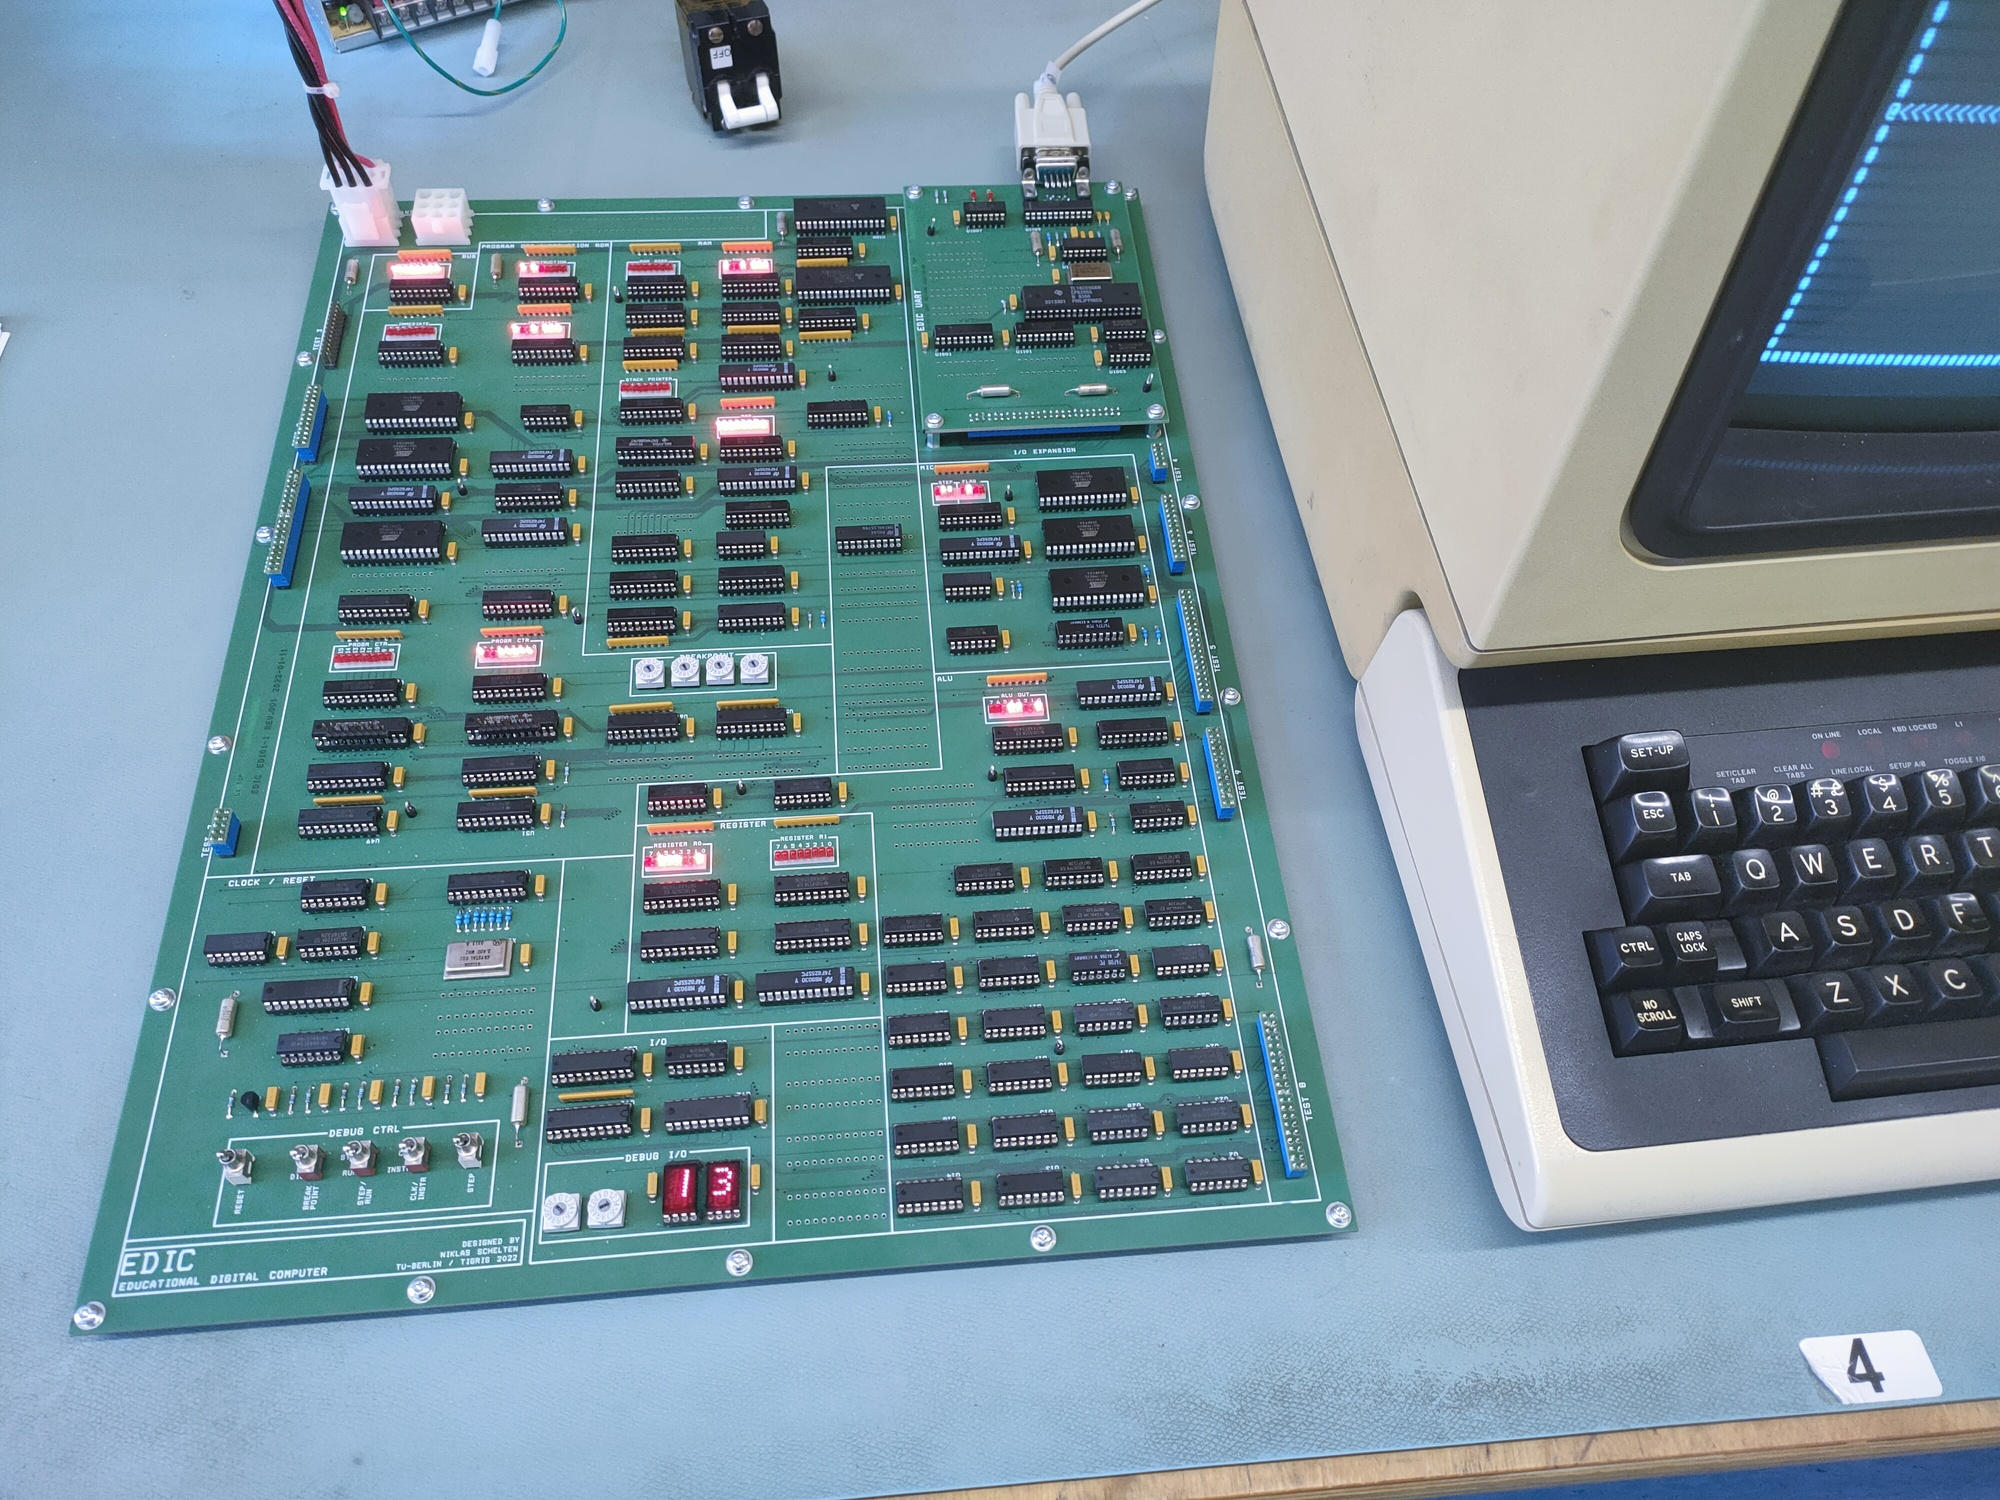
\includegraphics[width=\textwidth]{IMG20220308163628_resize.jpg}
  \caption{The final version of the \gls{EDiC} playing Snake on a VT-100 over an RS-232 I/O card.}
  \label{fig:EDiCSnake}
\end{figure}
\section{Background}
\subsection{Short History on Computing}
The history of computing hardware goes back to ancient times when people used devices like the abacus which simplifies calculations like additions or multiplications.
Starting from the end of the 19th century, analog computers were developed which used continuous physical phenomena to explore complex problems.
One of the first widespread analog computers was created by Sir William Thomson (Lord Kelvin) which predicted tide levels for particular locations by using a set of pulleys and wires. \cite{sep-computing-history}
Even though analog computers could perform very complex operations like solving differential equations \cite{analogDiff} they also had the major drawback that, due to their analog and continues nature, it was not possible to exactly recreate a calculation.

The idea of modern, digital computers was firstly theorized by Alan Turing in his paper \emph{On Computable Numbers} in 1936. \cite{10.1112/plms/s2-42.1.230}
He introduced the notion of a universal (Turing) machine which describes a machine that is provable capable of computing everything that is computable.
All the computers today are as capable as a turing machine which is expressed by calling them \emph{turing complete}.
This is with exception from their finite memory and limited number range.
The first digital computers from the mid 20th century were mechanical or electromechanical machines which combined basic switches like relays and mostly mechanical memory.
As fully electrical computers increased the switching frequencies, a lot of different number formats where emerging:
Opposed to analog computers where one signal, e.g. a voltage, \emph{represents} a value, it now needs to \emph{encode} a value.
In the nowadays common binary system one signal encodes either a 0 or a 1 (for example a low and high voltage) but a lot of different number systems where used like bi-quinary\footnote{Bi-quinary has one quinary signal encoding 0-4 or 5-9 depending on one binary signal encoding a low or high number. This allows two signals to encode a decimal digit similarly to some abacuses.}.

A variety of technologies where developed for fully electric computers like vacuum tubes or transistors.
After using discrete transistors, the advent of \glspl{IC} in the late 50th lead to a rapid acceleration of computer complexity and speed while reducing the power consumption drastically.
The series of \glspl{IC} which is the most relevant to this thesis is the \gls{TTL} 74 series.
It is a successor of one of the first \gls{TTL} \glspl{IC} developed by Texas Instruments in 1964 for military applications: The 5400 series. \cite{ICs}
The 5400 series of \glspl{IC} was specified for a temperature range from \qty{-55}{\celsius} to \qty{+125}{\celsius} and came in a ceramic \gls{SMD} and \gls{DIL} packaging to meet the high requirements of the military and space industries.
Each package included a set of basic logic circuits like 4 2-input NAND gates in the 5400N.
In 1966 the first \glspl{IC} of the 74 series were released which had the same functions but with a reduced temperature rating of \qty{0}{\celsius} to \qty{+70}{\celsius} and often came in plastic packaging for consumer applications.
In contrast to previous \gls{RTL}, these \gls{TTL} \glspl{IC} were capable of higher switching frequencies and lower power consumption due to a second transistor driving the high voltage level.
See \cref{sec:ttl} for a more in depth description of the workings of a \gls{TTL} gate.
As the 74 family of \glspl{IC} became larger with more complex \glspl{IC}, more advanced technologies, such as \gls{CMOS}, were also introduced into the family to further reduce the power consumption or increase the switching speeds.

With further advances in the complexity and integration of computing nodes, the first microprocessors were developed in the 70s with the famous Intel 4004 and 8080 in 1971 and 1974, respectively.
These processors combine all the logic required for a general purpose \gls{CPU} into one \gls{IC} usually exposing interfaces for connecting memories and user \gls{IO} logic.

\subsection{Technology Selection for the \gls{EDiC}}
The design goal for the \gls{EDiC} was to create a \gls{CPU} which aids the teaching of how \glspl{CPU} generally work.
To build a custom \gls{CPU}, many of the above-mentioned technologies were used for computer design, however, not all of them are equally suited for a model \gls{CPU}.
It was decided to use \gls{TTL} \glspl{IC} of the 74 family in the \gls{EDiC} for several reasons:
\begin{itemize}
  \item \emph{Complexity:} The \glspl{IC} of this family are complex enough to make it possible to build complex systems as a general-purpose \gls{CPU} with only about 100 chips.
  On the other hand, each individual \gls{IC} is easy to understand since it is kept quite simple, for example the 7400 has a basic interface of 12 pins for the four 2-input NAND gates plus GND and +5V pins.

  \item \emph{Speed:} In contrast to previous technologies such as electromechanical relays or \gls{RTL}, the 74 series is a lot faster, particularly the 74F subseries which is mainly used in the \gls{EDiC}.
  It is feasible to create complex designs with the 74F series with a clock frequency of several \unit{\mega\hertz}.
  However, at the same time, the clock frequency is not too high, so that special care must be taken when designing the \gls{PCB} which would be the case with higher frequency signals.

  \item \emph{Simplicity:} Working with the \glspl{IC} is fairly easy: No special tools -- except a soldering iron and oscilloscope -- are required to assemble and test the system.
  Especially the usage of sockets for the \glspl{DIP} simplifies the build because no \gls{IC} can overheat while soldering and all the \glspl{IC} can be replaced later on or while testing.
\end{itemize}

In contrast to previous and also later technology, the \gls{TTL} also stands out as the best suited one.
When trying to build a \gls{CPU} out of discrete transistors, not only the logical level needs to be respected but a lot of static and dynamic behavior of the transistors needs to be analyzed.
This complicates the design and prevents students from comprehending the \gls{CPU} on its logical level.
On the other side, more modern technologies became so abstract and complex to use that the comprehension of the internal workings of the \gls{CPU} could also be lost.
For example, when choosing \glspl{FPGA} as the driving technology, the work surrounding the technology quickly becomes more complex than the \gls{CPU} itself.
The \gls{FPGA} \glspl{IC} require special voltage levels and special care with the high frequency clock traces, are hard to solder with small pins, require complex build toolchains, cannot be debugged with an oscilloscope and so on.

Thus, the \gls{TTL} was the ideal technology level for creating a model \gls{CPU} which helps students understanding the workings of \glspl{CPU}.

\subsection{Workings of \gls{TTL}}\label{sec:ttl}
\begin{figure}[t]
  \centering
  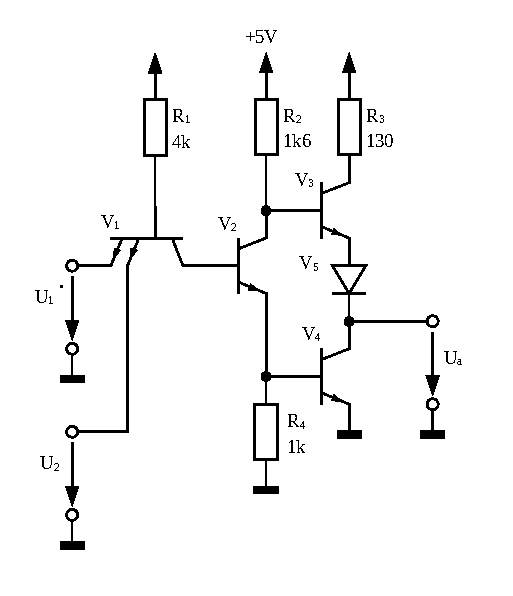
\includegraphics[width=\textwidth]{7400_Circuit.pdf}
  \caption{\gls{TTL} NAND with ``totem-pole'' output stage as in the 7400 \gls{IC}. \cite{7400_Circuit}}
  \label{fig:7400_Circuit}
\end{figure}

\Cref{fig:7400_Circuit} shows the internals of one of the four NAND gates inside the 7400 \gls{IC}.
The multi-emitter transistor $V_1$ functions as the logical NAND gate while the transistors $V_2$, $V_3$ and $V_4$ in combination with the diode $V_5$ form the ``totem-pole'' output stage.
If both inputs are high, a small collector current is drawn by both inputs because $V_1$ is in reverse-active mode.
The current through $R_1$ ``activates'' $V_2$ which in turn ``activates'' $V_4$ due to the current steering effect, where the current flows through the one parallel voltage-stable element with the lowest threshold voltage.
In this case, the current flows through $R_2$, $V_2$ collector-emitter and $V_4$ base-emitter rather than through $V_3$ collector-emitter, $V_5$ and $V_4$ collector-emitter.
Therefore, $V_4$ drives the output with a low voltage.

If one of the inputs is low, on the other hand, the current steering effect turns off $V_2$ since the current flows through $R_1$ and $V_1$ base-emitter rather than $R_1$, $V_1$ base-collector $V_2$ base-emitter and $R_4$.
Hence, the above-mentioned current steering effect on the output stage no longer takes effect and $V_3$ drives the output high through the diode $V_5$.

The advantage of this ``totem-pole'' output stage in comparison to a more simple output stage with the collector of $V_2$ effectively being the output is, that a very low output resistance can be achieved (only the small $R_3$) which allows the output to drive more inputs of other logic gates.
Additionally, the speed is drastically increased because the high output is actively driven instead of pulled up via a resistor as in \gls{RTL}.
However, the voltage drop over $V_3$ and $V_5$ also have the effect that the high output voltage is only about \qty{3.5}{\volt} in contrast to the simpler approach where almost \qty{5}{\volt} can be achieved.


\section{Thesis Structure}
Firstly, the following \cref{cha:architecture} will give an in-depth explanation of the \gls{CPU} architecture.
It includes an analysis of the design goals and explanations of how they can be achieved.
The individual modules are described as well as how they work together to execute any instruction.

Foccusing on usability, the \cref{cha:software} gives an overview of the software environment which eases the development of programs for the \gls{EDiC}.
Furthermore, it also features a tool with which the microcode for instructions can be changed, or new instructions can be added which is especially important looking at the educational purpose of the model \gls{CPU}.

Subsequently, \cref{cha:fpga} gives a short background to \glspl{FPGA} and then covers all the important aspects of the \gls{FPGA} model which was created to verify the architecture.
With a chip-level \gls{FPGA} implementation it was possible to not only verify the architecture but also the schematic of the \gls{EDiC} on the logical level.

In \cref{cha:hardware} the hardware design is finally detailed.
Besides an explanation of the schematics (attached in \cref{cha:schem}), the chapter also contains  information on the development process of the \gls{PCB} design.

After the \gls{PCB} was designed and produced, the process of testing the components and verifying all instructions is shown in \cref{cha:eval}.

A final conclusion and possibilities for further work are then given in \cref{cha:conclusion}.

% !TEX root = ../thesis.tex
\chapter{Architecture}\label{cha:architecture}
Designing and building a general purpose \gls{CPU} includes a lot of architectural decisions which will decide how well the \gls{CPU} performs, how complex it is and a lot more.
The goal for the \gls{EDiC} was to build a \gls{CPU} that is capable of basic basic interaction with an I/O device such as the VT-100 but at the same time simple enough to easily understand its workings, such that it may be used in education.
% For building the \gls{EDiC} the goal was to keep to the same basic infrastructure of the first version \gls{CPU}.
% However, many bugs and problems that occurred in the building of it should be addressed and avoided.
% Furthermore, the \gls{CPU} should be extended with some important features that were not implemented in the first version.

%%%%%%%%%%%%%%%%%%%%%%%%%%%%%%%%%%%%%%%%%%%%%
\section{Design Decisions}
First of all, there are several decisions about the general structure of a \gls{CPU} that need to be made.
These decisions greatly influence how the \gls{EDiC} can be structured into modules and how the final hardware build is setup.
Another important factor towards architectural structure is the fact that the final hardware build of the \gls{CPU} will be based on the 74-series of \glspl{IC}.

\subsection{8 bit bus width}
Most current era \glspl{CPU} employ a 32 bit or 64 bit bus to handle large numbers and large amounts of data.
This, however, is not feasible when using 74-series \glspl{IC} and at the same time targeting an easy to understand hardware build.
Some early \glspl{CPU} build with similar \glspl{IC} worked with only 4 bits.
This can work very well for specific applications but for the most arithmetics and data handling 8 bits are more practical.
The \gls{EDiC} will, therefore, use an 8 bit bus for data with a integer range of -128 to 127 or 0 to 255 for unsigned integers.

One of the major limitation of an overall 8 bit bus is the addressable memory space.
With only 8 bit for the memory address, the maximum amount of memory addressable is 256 bytes.
In the first version of the \gls{CPU} this limitation was extended a bit by providing 256 bytes of instruction memory besides 256 bytes of read only memory for instruction immediate values and 256 bytes of addressable \gls{SRAM}.
However, especially with a \gls{CISC} architecture, the limited \gls{SRAM} memory space greatly limits the overall complexity of programs that can be executed.
Additionally, more complex programs or even small operating systems are impossible to fit into 256 instructions.

Therefore, it was decided to extend the \gls{PC} and the memory addresses to 16 bit, which yields 65536 bytes of addressable \gls{SRAM} and theoretically 65536 instructions\footnote{The largest feasible \gls{EEPROM} available has only 15 address bits and with that only 32768 words of data.}.
However, this raises problems of where the 16 bit addresses come from when all the registers and the memory only store 8 bit.
The solution for the \gls{EDiC} is presented in \cref{sec:addrLogic} when explaining the different modules of the \gls{EDiC}.
\subsection{Datapath Architecture - Multicycle CISC}
In most \glspl{CPU} an instruction is not done in one clock cycle but it is divided into several steps that are done in sequence.
There are two general approaches that are called \emph{Multicycle} and \emph{Pipelining} \cite{PattersonDavid2016RuRD}.
Multicycle means that all the steps of one instruction are performed sequentially and a new instruction is only dispatched after the previous instruction is finished.
This is usually used when implementing \glspl{CISC}, where one instruction can be very capable \cite{chen_novick_shimano_2000}.
For example a add instruction in \gls{CISC} could fetch operands from memory, execute the add and write the result back to memory.
\glspl{RISC} on the other hand would need independent instruction to load operands from memory into registers, do the addition and write the result back to memory.

In Pipelining there a fixed steps each instruction goes through in a defined order and the intermediate results are stored in so called pipeline registers.
Each pipeline step is constructed in such a way that it does not intervene with the others.
Therefore, it is, in theory, possible to dispatch a new instruction each cycle even though the previous instruction is not yet finished.
A typically 5-step pipeline would consist of the following steps \cite{PattersonDavid2016RuRD}:
\begin{enumerate}
  \item \textbf{Instruction Fetch}: The instruction is retrieved from memory and stored in a register.
  \item \textbf{Instruction Decode}: The fetched instruction is decoded into control signals (and instruction specific data) for all the components of the \gls{CPU}.
  \item \textbf{Execute}: If arithmetic or logical operations are part of the instruction, they are performed.
  \item \textbf{Memory Access}: Results are written to the memory and/or data is read from memory.
  \item \textbf{Writeback}: The results are written back to the registers.
\end{enumerate}
However good the performance of a pipelined \gls{CPU} is, it also comes with challenges.
Those include a greater resource usage because all intermediate results need to be stored in pipeline registers.
Additionally, branch instructions\footnote{Branch Instructions change the \gls{PC} and with that the location from which the next instruction is to be fetched. This is required for conditional and looped execution.} pose a greater challenge because at the moment, the \gls{CPU} execute the branch the next instructions have already been dispatched.
This means that the pipeline needs to be flushed (i.e. cleared), performance is lost and more logic is required.
It also noteworthy that branch prediction and pipeline flushes can be quite vulnerable as recently shown in CVE-2017-5753 with the Spectre bug \cite{CVE-2017-5753}.

Therefore, the \gls{EDiC} is to built as a Multicycle \gls{CISC}.

\subsection{Single-Bus Oriented}
The decision for a Multicycle \gls{CPU} also enabled the architecture to be single-bus oriented.
This means that all modules (e.g. the \gls{ALU} or the memory) are connected to a central bus for data transfer.
The central bus is then used as a multi-directional data communication.
To allow this in hardware, all components that drive the bus (i.e. ``send'' data) need to have a tri-state driver.
A tri-state driver can either drive the bus with a defined `0' or `1' or high impedance which allows other tri-state drivers on the same bus to drive it.
That way an instruction which fetches a word from the memory from an address stored in a register, adds a register value to it and stores it in a register could consist of the following steps:
\begin{enumerate}
  \item Instruction Fetch
  \item Instruction Decode
  \item Memory Address from register over \emph{bus} to memory module
  \item Memory Access
  \item Data from memory module over \emph{bus} to \gls{ALU} input
  \item \gls{ALU} operation
  \item Data from \gls{ALU} output over \emph{bus} to register
\end{enumerate}
With such an architecture it is possible to avoid large multiplexers and keep the overall architecture simple.


\section{Modules}
The design has been split into 7 rather independent modules of varying complexity which mainly interface with the bus and control signals.
\subsection{\glsxtrfull{ALU}}\label{sec:alu}
\begin{table}
  \centering
  \renewcommand{\arraystretch}{1.25}
  \caption{Summary of the available alu operations.}
  \label{tab:aluOp}
  \begin{tabularx}{.8\textwidth}{ |c|c|c||X| }
    \hline
    aluOp[1] & aluOp[0] & aluSub & Resulting Operation             \\\hline\hline
    0        & 0        & 0      & ($A + B$) Addition              \\\hline
    0        & 0        & 1      & ($A - B$) Subtraction           \\\hline
    0        & 1        & 0      & ($A \land B$) AND               \\\hline
    0        & 1        & 1      & ($A \land \overline{B}$)        \\\hline
    1        & 0        & 0      & ($A \veebar B$) XOR             \\\hline
    1        & 0        & 1      & ($\overline{A \veebar B}$) XNOR \\\hline
    1        & 1        & 0      & ($A \gg B$) logical shift right \\\hline
    1        & 1        & 1      & ($A \ll B$) logical shift left  \\\hline
  \end{tabularx}
\end{table}
An \gls{ALU} is the operational core of any \gls{CPU} as it performs the calculations.
The \gls{ALU} of the \gls{EDiC} is by design simple with only 4 different operations plus an option to invert the second input.
The result of the \gls{ALU} is stored in a result register which can drive the bus to store the result in a register or memory.
For simplicity, the first input of the \gls{ALU} ($A$ input) is directly connected to the register file (\cref{sec:regs}) and only the second input ($B$ input) is accessible from the bus.
This limits the possibilities of instructions, however, if both inputs should have been driven by the bus, one input would have needed a register and every \gls{ALU} instruction would have taken two instead of one cycle.

The \gls{ALU} consists of an 8 bit ripple carry full adder and a barrel shifter.
The operations are controlled by three control signals: The first two bits select which \gls{ALU} operation to perform and the third bit modifies the operation to perform.
The possible operations are shown in \cref{tab:aluOp}.
For the adder, the third bit inverts the $B$ input when active (All input bits are XORed with the control bit) and is used as the carry in of the adder.
This essential subtracts the $B$ input from the $A$ input in two's complement arithmetic.
For the barrel shifter, the third bit reverses the shift direction.
\begin{figure}[t]
  \centering
  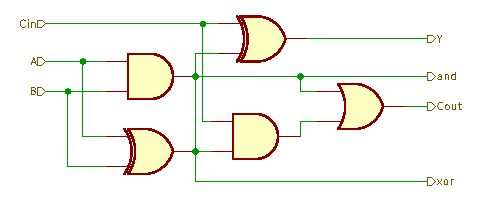
\includegraphics[width=\textwidth]{full_adder.pdf}
  \caption{1 bit full adder with the usual A, B and Carry inputs and Y and Carry outputs as well as the XOR and AND outputs.}
  \label{fig:full_adder}
\end{figure}
The XOR and AND operations shown in \cref{tab:aluOp} are chosen because they are already implemented in the half-adders and no additional logic is required to implement them.
A complete 1 bit full-adder of the \gls{EDiC} is shown in \cref{fig:full_adder}.

\begin{sidewaysfigure}[p]
  \centering
  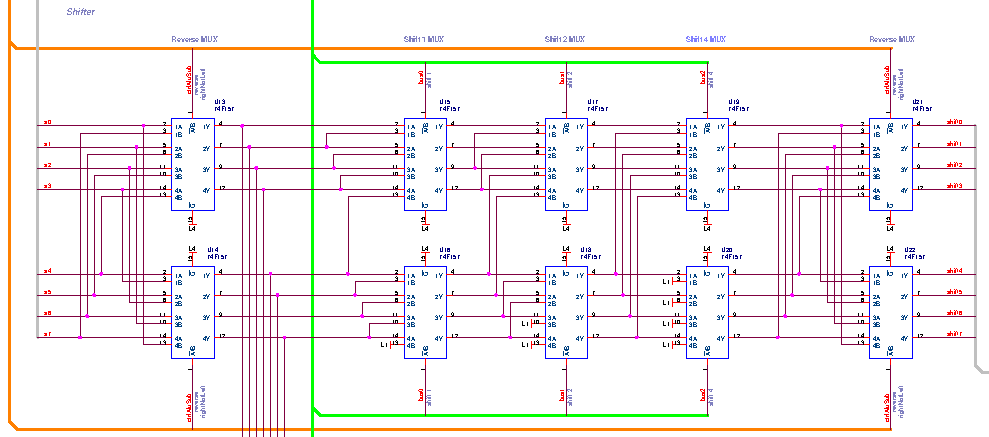
\includegraphics[width=\linewidth]{barrel_shifter.pdf}
  \caption{8 bit bidirectional barrel shifter.}
  \label{fig:barrel_shifter}
\end{sidewaysfigure}
It was desirable to include a barrel shifter to have the possibility to improve multiply operation with a shift and add approach instead of repeated addition.
The barrel shifter works by 3 consecutive multiplexers to shift by 1, 2 or 4 bit to the right that are controlled by the first 3 bit of the (not inverted) $B$ input.
To also allow shifting to the left there is one multiplexer before the three shift multiplexers to invert the order of bits and another one after the shifting to reorder the bits.
In \cref{fig:barrel_shifter} a bidirectional barrel shifter implemented with the \texttt{74F157} is visualized. The \texttt{74F157} implements four 2 to 1 multiplexer and, therefore, 2 chips are needed for a full 8 bit 2 to 1 multiplexer.

The \gls{ALU} also provides four flags which are used for condition execution.
The Zero (all result bits are zero) and Negative (The \gls{MSB} of the result) flag are both very easy to derive and were the only ones included in the first version of the \gls{CPU}.
However, the experience of programming for the \gls{CPU} showed that it is desireable to be able to work with more advanced \gls{ALU} flags when programming more complex functions.
Having only Zero and Negative Flags, for example, does not allow unsigned operations of the full width\footnote{An overflow and with that a greater or less than comparison cannot be done} which is especially important with only 8 data bits.
It limits unsigned operations to only 0-127 even though the \gls{ALU} would be capable of calculations with 0-255.

A lot of modern \glspl{CPU} feature many different flags with the Intel 64\textsuperscript{\textregistered} and IA-32 \gls{CPU} having about 20 different flags \cite[Section~3.4.3]{intelx86}.
However, the popular ARM Architecture has a rather unique but very capable system for conditional execution which relies on only the four most used \gls{ALU} flags.
The \gls{EDiC} uses the same flags and their functions are as follows:
\begin{itemize}
  \item \textbf{N} The \emph{Negative} flag indicates that the result is negative and is set if the 8th bit of the \gls{ALU} result is \texttt{'1'}.
  \item \textbf{Z} The \emph{Zero} flag indicates that the result is 0 and is set if all 8 result bits are 0.
  \item \textbf{V} The \emph{Overflow} flag indicates that an overflow occurred and is set if the carry in and carry out of the 8th full-adder are different.
  This detects arithmetic overflows for signed two's-complement calculations.
  \item \textbf{C} The \emph{Carry} flag is the carry out bit of the adder for adding and subtracting.
  For logical operations (\texttt{XOR} and \texttt{AND}) the carry flag has no meaning and for shifting operations it equals the last bit that was ``carried out'' (or is unchanged if shifting by 0 bits).
\end{itemize}
\subsection{Register File}\label{sec:regs}
As is typical with \glspl{CISC} the \gls{CPU} does not need many general purpose registers and the register file can be kept simple with only two registers.
The register file has one write port (from the bus) and two read ports of which one reads to the bus and the other is directly connected to the $A$ input of the \gls{ALU}.
All ports can access both registers.
\subsection{\glsxtrfull{PC} \& Instruction Register}
The \gls{PC} is a special 16 bit register which is used to store the address for the current instruction.
Usually it is incremented by one for each instruction.
However, it is also possible to load the \gls{PC} from an instruction immediate (see below) or from the memory (\cref{sec:memory}).
The first option is used for branch instruction while the second option is used for returning from a function, which is explained in more detail in \cref{sec:stack}.
The value of the \gls{PC} is used as address for the instruction \glspl{EEPROM} and can also be driven to the bus (lower 8 bits) and a second 8 bit memory line (\cref{sec:memory}) to store the \gls{PC} for function calls.

Each instruction of the \gls{EDiC} is stored in a 24 bit register of which 8 bits are the instruction and 16 bits represent an optional instruction immediate which can be used as an address for the memory/\gls{PC} (16 bit) or as data (8 bit) driven to the bus.
The instruction is directly forwarded to the control logic (\cref{sec:control}).
\subsection{Control Logic}\label{sec:control}
The control logic's job is to decode the current instruction and provide all the control signals for each cycle for any instruction.
For keeping track which cycle of each instruction is currently executing a 3 bit synchronous counter is needed.
Each control signal could be derived by a logical circuitry with 13 inputs: 8 bits instruction, 4 bits \gls{ALU} flags and 3 bits cycle counter.
However, designing these logic circuits is a lot of work, takes up a lot of space and cannot be changed easily later on. (For example when finding a bug in one instruction)
Therefore, an \gls{EEPROM} is used where the 13 bits that define one cycle of one specific instruction are used as addresses.
The control signals then are the data bits of the word that is stored at the specific address in the \gls{EEPROM}.
How the \gls{EEPROM} is programmed with the correct data is explained in depth in \cref{sec:microcode}.

One special case are the 3 bits \gls{ALU} opcodes.
They are not decoded the usual way from the instruction but are directly take from the 3 \glspl{LSB} of the instruction.
This is done to reduce the storage requirements for the decoding \glspl{EEPROM}.
For instructions that use the \gls{ALU}, the 3 \glspl{LSB} need to be set accordingly but for all other instructions, the three bits can be used as usual for decoding the instruction because it does not matter what the combinatorial part of \gls{ALU} does.

The first two cycles of each instruction need to be taken in special consideration because the instruction register is not yet loaded with the next instruction, because it is still being fetched and decoded.
However, the instruction fetch and decode are always the same for each instruction, which means that all memory locations where the cycle counter is equal to 0 or 1 (the first two instructions) are filled with the control signals for an instruction fetch and decode.
\subsection{Memory}\label{sec:memory}
The memory module became the most complex module because it includes not only the main memory of the \gls{CPU} in form of an asynchronous \gls{SRAM} but also includes a lot of addressing logic for the 16 bit addresses.

The addressing logic is required because the \gls{EDiC} has 16 bit address with only an 8 bits data bus.
However, the \gls{EDiC} also features memory mapped I/O and a stack implementation which further complicate the addressing logic.
Both these features and the result logic is described below.

\subsubsection{Memory Mapped I/O}
Input and Output is one of the most important factors of any \gls{CPU} besides the computing capabilities which are mostly defined by the \gls{ALU}.
Using individual instructions for I/O which directly read from and write to the bus are limiting the usability quite a lot.
A common way to extend the I/O capabilities is to use so called Memory Mapped I/O.
This works by splitting the address space between actual memory and I/O devices.
Then every I/O operation is performed as a usual memory access but the memory chip does not receive the access and the I/O device addressed performs the operation.
In the \gls{EDiC} the memory address is decoded in such a way, that accesses to addresses \texttt{0xfe00} to \texttt{0xfeff} are performed by any connected I/O devices.
For this to work, the lower 8 address bits, the bus and memory control signals - i.e. write enable, read enable and I/O chip enable (active when the upper 8 address bits are \texttt{0xff}) - are exposed for I/O devices to connect to.
\subsubsection{Stack Implementation}\label{sec:stack}
A feature that has been thoroughly missing from the first \gls{CPU} version is a kind of stack implementation.
The stack is essential to the workings of the programming paradigm \emph{functions}.
When calling functions, the return address is usually (automatically) stored on the stack where also local variables can be stored.
This allows functions to be called recursively and also simplifies the written assembler compared to simple branching.

However, a typical stack implementation as in modern \gls{CPU} architectures like ARM is rather complex.
It requires a \gls{SP} register which usually is accessible like any other general purpose register and can be directly used as an address.
This includes using it as operand for arithmetic operations which is not possible when the bus width is only 8 bits but the \gls{SP} needs to be16 bits wide to be used as an address.
Therefore, the \gls{EDiC} uses an unique approach to the stack:

Similarly to the memory mapped I/O it was decided to implement the stack as an 8 bit register which can be incremented and decremented.
Every time a memory access is performed where the upper 8 bits of the address equal \texttt{0xff}, a 17th address bit is set and the upper 8 address bits are replaced by the current value of the \gls{SP}.
For example: The \gls{SP}  is currently \texttt{0x21} and a memory access to the address \texttt{0xff42} is performed.
Then the actual address at the memory \gls{IC} is \texttt{0x1\_2142}.

This allows each function (which has a unique \gls{SP} value on the current call stack) to have 256 bytes of function local memory.
In the \emph{call} instruction, the \gls{EDiC} automatically stores the return address (next \gls{PC} value) at address \texttt{0xffff}, which is \texttt{0x1\_\{sp\}ff} after translation.
To store the whole 16 bit return address, a second memory \gls{IC} is used in parallel which only needs 256 bytes of storage.
In the hardware build of the \gls{EDiC} the same \gls{SRAM} \gls{IC} as for the main memory is used because it is cheaply available and the built is simplified by not using more different components.
The call and return instructions are further described in \cref{sec:instructionSet}.

Usually, the stack is also used to store parameters for a function call.
In the \gls{EDiC}, this can be achieved by providing a special \emph{store} and \emph{load} instruction which access the stack memory with an increment \gls{SP}.
This way it is possible to store parameter before calling a function and it is also possible to retrieve modified values after the call\footnote{This is important when a function takes memory pointers as parameters and modifies them. For example a string parsing function could take a pointer to the start of the string, parse some characters as a number, return its number representation and modify the parameter such that it points to where the parsing stopped.}
\subsubsection{Addressing Logic}\label{sec:addrLogic}
With increasing the address width to 16 bit and also adding more functionality to the memory access, the addressing logic has become more complex.
There are two main sources for memory addresses: The new 16 bit \gls{MAR} which can be written to from the bus and the 16 bit instruction immediate.
As the bus is only 8 bits wide, there is a special instruction to write to the upper 8 bits of the \gls{MAR} and the lower bits are written in the memory access instruction.
This can be used when a memory address is stored in registers and is needed when looping through values in the memory like arrays.
When accessing addresses known at compile time, the instruction immediate can be used as an address which has been extended to support 16 bit.
These two sources of addresses are then decoded to either select the stack (upper 8 bits equal \texttt{0xff}), memory mapped I/O (\texttt{0xfe}) or regular memory access.
The chip enable of the main memory is only asserted when performing stack and regular memory accesses while the I/O chip enable is only asserted when the upper 8 bits are \texttt{0xfe}.
Additionally, the 17th address bit is asserted when stack access is performed and the upper 8 bits of the address are replaced with the \gls{SP} in this case.

\subsection{Input \& Output}\label{sec:IO}
The \gls{EDiC} can interface with different I/O devices connected to it via the memory mapped I/O.
For evaluation and debugging, the \gls{EDiC} includes one I/O device at address \texttt{0x00} which can be read from and written to.
The values to be read can be selected by the user with a hexadecimal 8 bit switch and the values written to the address \texttt{0x00} are displayed with a 2 digit display.
This allows simple programs to run independently of external I/O devices.

\subsection{Clock, Reset \& Debugging}\label{sec:clock}
An important feature when developing a \gls{CPU} is debugging capabilities.
The initial version could at least step the clock cycle by cycle.
However, as programs get complexer this feature quickly becomes less useful as each instruction is made of several cycles and when a problem occurs after several hundred instructions it is infeasible to step through all cycles.
Additionally, the usual application developer does not want to step through each cycle but rather step through each instruction, assuming that the instruction set works as intended.
Another important debugging feature is the use of breakpoints where the \gls{CPU} halts execution when the \gls{PC} reaches a specific address.

In the \gls{EDiC} halting was not realized by stopping the clock completely but rather by inhibiting the instruction step counter increment.
This has the advantage that the clock is not abruptly pulled to 0 or 1 and, therefore, no spikes on the clock line can occur.
To implement a cycle by cycle stepping mode, the halt signal is de-asserted for only one clock cycle, which in turn increments the step counter only once.
To step whole instructions, the halt signal is de-asserted until the instruction is finished (marked by a control signal that is asserted at the end of each instruction from the control logic).
In breakpoint mode, the halt signal is controlled from a comparator that compares the \gls{PC} and a 16 bit user input, asserting the halt signal when those two equal.
As soon as the \gls{CPU} halts, the user can then switch to stepping mode and debug the specific instruction of the program.
The user can freely switch between these modes with switches and buttons.
\section{Control Signals}\label{sec:controlSignals}
\TODO{explain control signals}
\section{Final Instruction Set}\label{sec:instructionSet}
This section describes all available instructions, what they do and which instruction cycle performs which steps of the instruction.
Each instruction starts with the same two cycles for instruction fetching.
The following instructions are supported by the hardware:
\subsection{\gls{ALU} operations}
The \gls{EDiC} supports a wide variety of instructions that perform \gls{ALU} operations.
All these operations take two arguments which are used for one of the possible operations shown in \cref{tab:aluOp}.
Each \gls{ALU} operation modifies the status flags.
\begin{itemize}
  \item \emph{Register x Register:} Takes two registers as parameter and the result is stored in the first parameter.

  Cycles:
  \begin{enumerate}
    \item Both register to \gls{ALU} A and B input, write enable of \gls{ALU} result register.
    \item Write content of \gls{ALU} result register into first parameter register.
  \end{enumerate}

  \item \emph{Register x Register (no write back):} Takes two registers as parameter and the result is only calculated for the status flags.

  Cycles:
  \begin{enumerate}
    \item Both register to \gls{ALU} A and B input, write enable of \gls{ALU} result register.
  \end{enumerate}

  \item \emph{Register x Memory (from Register):} Takes one register as \gls{ALU} A input and a second register which is used as a memory address for the \gls{ALU} B input.
  The result is stored in the first register.

  Cycles:
  \begin{enumerate}
    \item Second register is stored in the lower 8 bits of the \gls{MAR}\footnote{The upper 8 bits of the \gls{MAR} should be set beforehand}.
    \item Address calculations.
    \item First register and memory content as A and B inputs, write enable of the result register.
    \item Write content of \gls{ALU} result register into first parameter register.
  \end{enumerate}

  \item \emph{Register x Memory (from immediate):} Takes one register as \gls{ALU} A input and a 16 bit value as immediate which is used as a memory address for the \gls{ALU} B input.
  The result is stored in the first register.

  Cycles:
  \begin{enumerate}
    \item Address calculations.
    \item First register and memory content as A and B inputs, write enable of the result register.
    \item Write content of \gls{ALU} result register into first parameter register.
  \end{enumerate}

  \item \emph{Register x Memory (from immediate, no write back):} Takes one register as \gls{ALU} A input and a 16 bit value as immediate which is used as a memory address for the \gls{ALU} B input.
  The result is only calculated for the status flags.

  Cycles:
  \begin{enumerate}
    \item Address calculations.
    \item First register and memory content as A and B inputs, write enable of the result register.
  \end{enumerate}

  \item \emph{Register x Immediate:} Takes one register as \gls{ALU} A input and an 8 bit value as immediate  for the \gls{ALU} B input.
  The result is stored in the first register.

  Cycles:
  \begin{enumerate}
    \item Register and immediate value as A and B inputs and write enable of the result register.
    \item Write content of \gls{ALU} result register into first parameter register.
  \end{enumerate}

  \item \emph{Register x Immediate (no write back):} Takes one register as \gls{ALU} A input and an 8 bit value as immediate  for the \gls{ALU} B input.
  The result is only calculated for the status flags.

  Cycles:
  \begin{enumerate}
    \item Register and immediate value as A and B inputs and write enable of the result register.
  \end{enumerate}
\end{itemize}

\subsection{Memory operations} Some \gls{ALU} operations also include reading values from memory.
However, the \gls{EDiC} features a lot more memory operations which are detailed below.
As all memory operations may perform memory mapped I/O operations, special care must be taken to allow asynchronous I/O devices to function as well.
This means that for each memory access, the address setup and hold must be an individual cycle, resulting in a 3 cycle memory access.
\begin{itemize}
  \item \emph{Load from register address:} Takes the second register parameter as the lower 8 bits of the memory address and writes the memory content to the first register.

  Cycles:
  \begin{enumerate}
    \item Second register to lower \gls{MAR}.
    \item Memory address setup.
    \item Memory read access and write back to first register.
    \item Memory address hold.
  \end{enumerate}

  \item \emph{Load from immediate address:} Takes a 16 bit immediate as the memory address and writes the memory content to the register.

  Cycles:
  \begin{enumerate}
    \item Memory address setup.
    \item Memory read access and write back to first register.
    \item Memory address hold.
  \end{enumerate}

  \item \emph{Load from immediate address with incremented \gls{SP}:} Takes a 16 bit immediate as the memory address and writes the memory content to the register.
  However, before the memory access, the \gls{SP} is incremented and after the access, the \gls{SP} is decremented again.
  This is used to access parameters for subfunctions.

  Cycles:
  \begin{enumerate}
    \item Increment Stack Pointer.
    \item Memory address setup.
    \item Memory read access and write back to first register.
    \item Memory address hold.
    \item Decrement Stack Pointer.
  \end{enumerate}

  \item \emph{Store to register address:} Takes the second register parameter as the lower 8 bits of the memory address and writes the content of the first register to the memory.

  Cycles:
  \begin{enumerate}
    \item Second register to lower \gls{MAR}.
    \item Memory address and data setup.
    \item Memory write access.
    \item Memory address and data hold.
  \end{enumerate}

  \item \emph{Store to immediate address:} Takes a 16 bit immediate as the memory address and writes the register content to memory.

  Cycles:
  \begin{enumerate}
    \item Memory address and data setup.
    \item Memory write access.
    \item Memory address and data hold.
  \end{enumerate}

  \item \emph{Store to immediate address with incremented \gls{SP}:} Takes a 16 bit immediate as the memory address and writes the register content to memory.
  However, before the memory access, the \gls{SP} is incremented and after the access, the \gls{SP} is decremented again.
  This is used to access parameters for subfunctions.

  Cycles:
  \begin{enumerate}
    \item Increment Stack Pointer.
    \item Memory address and data setup.
    \item Memory write access.
    \item Memory address and data hold.
    \item Decrement Stack Pointer.
  \end{enumerate}

  \item \emph{Set upper 8 bits of \gls{MAR} from register:} Sets the upper \gls{MAR} register to the content of the register.

  Cycles:
  \begin{enumerate}
    \item Register output enable and upper \gls{MAR} write enable.
  \end{enumerate}

  \item \emph{Set upper 8 bits of \gls{MAR} from immediate:} Sets the upper \gls{MAR} register to the 8 bit immediate value.

  Cycles:
  \begin{enumerate}
    \item Immediate output enable and upper \gls{MAR} write enable.
  \end{enumerate}
\end{itemize}

\subsection{Miscellaneous operations}
There are some more operations that are strictly speaking neither \gls{ALU} nor memory operations like moves and branches.
\begin{itemize}
  \item \emph{Move between register:} Set the first register to the value of the second.

  Cycles:
  \begin{enumerate}
    \item Second register output enable and first register write enable.
  \end{enumerate}

  \item \emph{Move immediate to register:} Set the register to the value of the immediate.

  Cycles:
  \begin{enumerate}
    \item Immediate output enable and first register write enable.
  \end{enumerate}

  \item \emph{Conditionally set \gls{PC} from immediate:} This is the only conditional operation available.
  Depending on the current status register the following cycles are either executed or \glspl{NOP} are executed.

  Cycles:
  \begin{enumerate}
    \item \gls{PC} write enable from immediate.
  \end{enumerate}

  \item \emph{Function Call:} Takes a 16 bit address which the \gls{PC} is set to.
  The \gls{SP} is incremented and the return address is stored on the stack.

  Cycles:
  \begin{enumerate}
    \item Increment \gls{SP} and write \texttt{0xffff} into the \gls{MAR}.
    \item Memory address and data (\gls{PC}) setup.
    \item Memory write access.
    \item Memory address and data hold.
    \item Load \gls{PC} from instruction immediate.
  \end{enumerate}

  \item \emph{Function Return:} Decrements the \gls{SP} and the \gls{PC} is loaded from the return address which is read from the memory.

  Cycles:
  \begin{enumerate}
    \item Write \texttt{0xffff} into the \gls{MAR}.
    \item Memory address setup.
    \item Memory read access and \gls{PC} write enable.
    \item Memory address hold.
    \item Decrement \gls{SP}.
  \end{enumerate}
\end{itemize}
% !TeX root = ../thesis.tex
\chapter{Software Development Environment}\label{cha:software}
When just providing the hardware, the \gls{CPU} can hardly be used.
It is possible to write programs by hand by writing single bytes to the \glspl{EEPROM} that hold the program.
However, it is quite infeasible to write complex programs this way.
While manually writing programs byte by byte is doable, writing the content of the \glspl{EEPROM} which hold the microcode by hand is quite infeasible.

Therefore, the \gls{EDiC} comes with two main software utilities that form the software development environment in \cref{sec:microcode,sec:assembler}.

\section{Microcode Generation}\label{sec:microcode}
\begin{listing}[t]
  \inputminted[linenos,
    breaklines,
    frame=leftline,
    xleftmargin=20pt,
  ]{TypeScript}{src/microcode.ts}
  \caption{Schema of the Microcode Definition CSON-File \cite{CSON} as a TypeScript \cite{TS} Type definition.}
  \label{lst:micrcode_schema}
\end{listing}
The goal is to define all the available instructions and what they perform in which instruction step and then have a program automatically generate the bit-files for the \gls{EEPROM}.
This approach allows simple modifications to the existing microcode if a bug was found or a new instruction should be added.
The file format which defines the microcode has to be human and machine-readable as it should be easily edited by hand and also be read by the tool that generates the bit-files.
A very common file format for tasks like this is \gls{JSON} \cite{JSON} which is widely used in the computer industry.
Besides basic types as strings and numbers, it allows arrays with square brackets (\texttt{[]}) and objects with curly braces (\texttt{\{\}}).
Each object contains key value pairs and everything can be nested as desired.
For the \gls{EDiC} microcode generation \gls{CSON} was used which is very similar to \gls{JSON} but is slightly easier to write by hand because its syntax is changed a bit:
\begin{itemize}
  \item It allows comments which is extensively used to ease the understanding of individual instruction steps.
  \item Braces and commas are not required.
  \item Keys do not require string quotation marks.
\end{itemize}
The schema for the file describing the microcode is shown in \cref{lst:micrcode_schema}.
Some examples for the fields are listed below:
\paragraph{Signals}
\begin{listing}[t]
\begin{sublisting}[b]{.5\textwidth}
  \begin{minted}[linenos,
    breaklines,
    frame=leftline,
    xleftmargin=20pt,
  ]{CoffeeScript}
{
  name: 'reg0NWE'
  noOp: 1
}
  \end{minted}
  \caption{Register 0 write enable control signal.}
  \label{lst:mc_signals}
\end{sublisting}
\begin{sublisting}[b]{.45\textwidth}
  \begin{minted}[linenos,
    breaklines,
    frame=leftline,
    xleftmargin=20pt,
  ]{CoffeeScript}
instructionFetch: [
  { # write instruction
    memInstrNWE: 0
  }
  { # increment PC
    memPCNEn: 0
    memPCLoadN: 1
  }
]
  \end{minted}
  \caption{Instruction fetch and decode cycles.}
  \label{lst:mc_instrFetch}
\end{sublisting}
\caption{Example definitions of one control signal and the instruction fetch cycles for the microcode generation.}
\end{listing}
The signals array consists of objects that define the available control signals and the default value of the control signal.
\Cref{lst:mc_signals} defines the \emph{not write enable signal for register 0} control signal and defines the default state as high.
This means, when this control signal is not specified in an instruction it will stay high and, therefore, register 0 will not be written.

\paragraph{Instruction Fetch} This array defines the steps that are performed at the beginning of each instruction to fetch the new instruction and decode it.
Each object represents one step and consists of key value pairs that define one control signal.

In \cref{lst:mc_instrFetch} the first instruction cycle specifies only the \emph{instruction not write enable} to be low and with this write the instruction into the instruction register.
Secondly, the \gls{PC} is incremented by setting \emph{PC not enable} to low and \emph{PC not load} to high.
\paragraph{Instructions} The instructions are an array of all available instructions.
Each instruction is defined as an op code, which is the 8 bit instruction in binary format.
However, if it was only possible to define the 8 bit as 0s and 1s, instructions which only differ in the register used would need to be specified separately which is very error-prone.
Therefore, it is allowed to specify the bit that determines if register 0 or 1 is used to be set to \texttt{'r'} or \texttt{'s'} and then multiple instructions are generated.
The \texttt{cycles} array defines the steps each instruction does in the same way as the \texttt{instructionFetch} array does.
However, as the value of individual control signals may depend on which register is specified in the op code, it is also possible to specify \texttt{'r'}, \texttt{'!r'}, \texttt{'s'} or \texttt{'!s'}.

\begin{listing}[t]
  \begin{sublisting}[b]{.45\textwidth}
    \begin{minted}[linenos,
      breaklines,
      frame=leftline,
      xleftmargin=20pt,
    ]{CoffeeScript}
{
  op: '1111100r' # r = imm
  cycles: [
    { # imm to bus to r
      reg0NWE: 'r'
      reg1NWE: '!r'
      memInstrNOE: 0
    }
  ]
}
    \end{minted}
    \caption{Definition using `r' in the opcode.}
    \label{lst:mc_movImm}
  \end{sublisting}
  \begin{sublisting}[b]{.5\textwidth}
    \begin{minted}[linenos,
    breaklines,
    frame=leftline,
    xleftmargin=20pt,
    ]{CoffeeScript}
[
  {
    op: '11111000' # r0 = imm
    cycles: [
      { # imm to bus to r0
        reg0NWE: 0
        reg1NWE: 1
        memInstrNOE: 0
      }
    ]
  }
  {
    op: '11111001' # r1 = imm
    cycles: [
      { # imm to bus to r1
        reg0NWE: 1
        reg1NWE: 0
        memInstrNOE: 0
      }
    ]
  }
]
    \end{minted}
    \caption{Equivalent definition of both separate instructions.}
    \label{lst:mc_movImmDuplicate}
  \end{sublisting}
  \caption{Definition of the move immediate to register instruction for the microcode generation.}
\end{listing}
\Cref{lst:mc_movImm} defines the move immediate to register instruction for both register at the same time.
The \emph{instruction immediate not output enable} is low and either register 0 or register 1 is written to.
This definition would be equal to \cref{lst:mc_movImmDuplicate}.

This example is quite simple, however, instructions with two registers as arguments would result in four times the same definition and duplication can always result in inconsistencies.
The same idea is also used for the \gls{ALU} operations.
The \gls{ALU} operation control signals are not generated by the microcode but are rather the three least significant bits of the instruction.
Therefore, all instructions using the \gls{ALU} can have the exact same control signals stored in the microcode \gls{EEPROM}.
To avoid 8 definitions of the same instructions, the op code can contain \texttt{'alu'} and all 8 instructions are generated.
\begin{listing}[h!]
  \begin{minted}[linenos,
    breaklines,
    frame=leftline,
    xleftmargin=20pt,
  ]{CoffeeScript}
{
  op: '000rsalu' # r = r x s (alu)
  cycles: [
    { # r x s into alu
      aluYNWE: 0
      reg0BusNOE: 's'
      reg1BusNOE: '!s'
      regAluSel: 'r'
    }
    { # alu into r
      aluNOE: 0
      reg0NWE: 'r'
      reg1NWE: '!r'
    }
  ]
}
  \end{minted}
  \caption{Definition of the \gls{ALU} operation with two register arguments for the microcode generation.}
  \label{lst:mc_aluRS}
\end{listing}
\Cref{lst:mc_aluRS} for example defines the \gls{ALU} operation with two registers and defines all 32 instructions with the op codes \texttt{'00000000'} to \texttt{'00011111'}.

\begin{listing}[h!]
  \begin{minted}[linenos,
    breaklines,
    frame=leftline,
    xleftmargin=20pt,
  ]{CoffeeScript}
{
  op: '1010flag' # pc := imm
  cycles: [
    { # imm to pc
      memPCNEn: 0
      memPCLoadN: 0
      memPCFromImm: 1
    }
  ]
}
  \end{minted}
  \caption{Definition of the branch instructions.}
  \label{lst:mc_branch}
\end{listing}
There is one final specialty built into the Microcode Generator:
The \gls{EDiC} has a branch instruction which is either executed or treated as a no-operation depending on the current state of the \gls{ALU} flags.
For all other instructions, the flags are ignored, and the instructions are always executed.
For this special instruction, the last four bits replaced with \texttt{flag} define at which state of the \gls{ALU} flags, the branch should be executed.
The possible conditions are heavily inspired by the conditional execution of ARM \glspl{CPU}\cite{armCond} as the \gls{ALU} flag architecture is very similar.
The possible values for the \texttt{flag} field and their meanings are listed in \cref{tab:mc_flagMeanings}.
Especially for a \gls{CPU} with only 8 bits it is important to support unsigned and signed operations and with a complex microcode it is no problem to support all the different branch instructions and facilitate the application design.
\Cref{lst:mc_branch} defines the branch instructions.
\begin{table}[t]
  \centering
  \renewcommand{\arraystretch}{1.25}
  \caption{All available branch instructions with their op-code and microcode translation based on the \gls{ALU} flags explained in \cref{sec:alu}.}
  \label{tab:mc_flagMeanings}
  \begin{tabularx}{\textwidth}{ |c|l|l|X| }
    \hline
    \texttt{flag} (OP-Code) & Assembler Instruction                & \gls{ALU} flags                 & Interpretation   \\\hline\hline
    \texttt{0000}           & \texttt{jmp}/\texttt{bal}/\texttt{b} & Any                             & Always           \\\hline
    \texttt{0001}           & \texttt{beq}                         & \texttt{Z==1}                   & Equal            \\\hline
    \texttt{0010}           & \texttt{bne}                         & \texttt{Z==0}                   & Not Equal        \\\hline
    \texttt{0011}           & \texttt{bcs}/\texttt{bhs}            & \texttt{C==1}                   & Unsigned $\geq$  \\\hline
    \texttt{0100}           & \texttt{bcc}/\texttt{blo}            & \texttt{C==0}                   & Unsigned $<$     \\\hline
    \texttt{0101}           & \texttt{bmi}                         & \texttt{N==1}                   & Negative         \\\hline
    \texttt{0110}           & \texttt{bpl}                         & \texttt{N==0}                   & Positive or Zero \\\hline
    \texttt{0111}           & \texttt{bvs}                         & \texttt{V==1}                   & Overflow         \\\hline
    \texttt{1000}           & \texttt{bvc}                         & \texttt{V==0}                   & No overflow      \\\hline
    \texttt{1001}           & \texttt{bhi}                         & \texttt{C==1} and \texttt{Z==0} & Unsigned $>$     \\\hline
    \texttt{1010}           & \texttt{bls}                         & \texttt{C==0} or \texttt{Z==1}  & Unsigned $\leq$  \\\hline
    \texttt{1011}           & \texttt{bge}                         & \texttt{N==V}                   & Signed $\geq$    \\\hline
    \texttt{1100}           & \texttt{blt}                         & \texttt{N!=V}                   & Signed $<$       \\\hline
    \texttt{1101}           & \texttt{bgt}                         & \texttt{Z==0} and \texttt{N==V} & Signed $>$       \\\hline
    \texttt{1110}           & \texttt{ble}                         & \texttt{Z==0} or \texttt{N!=V}  & Signed $\leq$    \\\hline
    \texttt{1111}           & -                                    & Any                             & Never (Not used) \\\hline
  \end{tabularx}
\end{table}

\section{Assembler}\label{sec:assembler}
The second software that is similarly important is the assembler.
An assembler translates human-readable instructions into machine code, i.e. the bits that are stored in the instruction \glspl{EEPROM}.
For the \gls{EDiC} each instruction is 24 bits wide, with 8 bits instruction op code and 8 or 16 bits immediate value.
Even though assemblers usually only translate instructions one by one, they can have quite advanced features.
With an assembler, the programmer is no longer required to know the specific op codes for all instructions and set individual bits of the instructions which is very error-prone.
The assembler for the \gls{EDiC}, therefore, allows easier programming with a simple text-based assembly syntax similar to the well-known ARM syntax.
\begin{listing}[t]
  \inputminted[linenos,
    breaklines,
    frame=leftline,
    xleftmargin=20pt,
  ]{ARM}{src/prng.s}
  \caption{\gls{PRNG} written in the \gls{EDiC} Assembler.}
  \label{lst:asm_prng}
\end{listing}

\begin{listing}[t]
  \inputminted[linenos,
    breaklines,
    frame=leftline,
    xleftmargin=20pt,
  ]{ARM}{src/prng_out.s}
  \caption{The output of the \gls{PRNG} of \cref{lst:asm_prng}. The first 16 bits are the memory address, then 8 bits for the instruction op-code and 16 bits for the instruction immediate follow. For reference, the original instruction with all the variables replaced is appended.}
  \label{lst:asm_prng_out}
\end{listing}

\Cref{lst:asm_prng,lst:asm_prng_out} show the translation that the assembler does.
In particular, \cref{lst:asm_prng} shows the assembler program that is written by the programmer and \cref{lst:asm_prng_out} summarizes what values are stored in the program \gls{EEPROM}.

The full assembler code used in the demonstration in \cref{fig:EDiCSnake} is attached in \cref{cha:schem}.

\subsection{Calling conventions}\label{sec:callingConvention}
Even though calling conventions are strictly speaking not a feature of the assembler, it is an important factor to keep in mind in functional programming.
Calling conventions are a set of rules which caller (the instructions calling a subroutine) and callee (the subroutine that is called) should usually follow.
\paragraph{Parameters}
Typically, the first parameters from the caller to the callee are passed in registers, which avoids long memory operations for storing and loading the parameters.
As the \gls{EDiC}'s memory operations cannot stall they are not slower than register operation and the \gls{EDiC} has only 2 registers.
Therefore, only the very first argument is passed in \texttt{r0} and all further arguments are passed in the memory.
The parameters are stored on the stack of the callee starting at stack address \texttt{0x00} (\texttt{0xff00} as memory address).
\paragraph{Return value}
The return value is to be placed in \texttt{r0}.
If a return value larger than 8 bit (or multiple 8 bit values) are to be returned, the caller may pass a pointer to a memory location as a parameter and the callee works on the memory content pointed to.
\paragraph{Preservation}
The register \texttt{r1} can be used as a function local variable and, therefore, has to be preserved by any callee.
This is usually done by storing the content on the stack at the beginning of the function and restoring it from the stack at the end of the function.

\subsection{Available Instructions}\label{sec:asm_instr}
This section summarizes all available instructions and which parameters they take.
All instructions start with the operation followed by up to two parameters which are separated by a comma.

There are four different parameter types.
It can either be a register specified as \texttt{r0} or \texttt{r1}.
The register value can also be passed as the address to a memory operation with \texttt{[r0]}.

Immediate values can also be specified as value or as address with brackets around the immediate value.
However, the syntax for immediate values is more complex, as the assembler can parse decimal (positive and negative) as well as hexadecimal numbers.
Additionally, variables can be used which are further explained in \cref{sec:constants}.

When specifying a value, the immediate can range between -127 and 255 (two's complement and unsigned) and when used as an address it can range between 0 and 0xfffe (65534). The upper limit is not 0xffff because that address is reserved for the return address and should not be overwritten.
\subsubsection{\glsxtrshort{ALU} Instructions}
The following \gls{ALU} instructions are available:
\begin{multicols}{4}
  \begin{itemize}
    \item add
    \item sub
    \item and
    \item eor
    \item xor
    \item xnor
    \item lsr
    \item lsl
  \end{itemize}
\end{multicols}
\gls{ALU} instructions always take two parameters.
The first parameter is the left hand side operand and the register where the result is stored in, and the second parameter is the right hand side operand.
The following operand combinations are possible:
\begin{itemize}
  \item Two registers

        \qquad\mintinline{ARM}{sub r0, r1} does: $r_0:=r_0-r_1$
  \item One register and one register as memory address

        \qquad\mintinline{ARM}{lsr r1, [r0]} does: $r_1:=r_1\gg\text{mem}[r_0]$
  \item One register and an immediate value

        \qquad\mintinline{ARM}{xor r0, 0x0f} does: $r_0:=r_0\xor 15$
  \item One register and an immediate value as memory address

        \qquad\mintinline{ARM}{add r1, [0x0542]} does: $r_1:=r_1+\text{mem}[1346]$
\end{itemize}
All the \gls{ALU} instructions can have an `s' as suffix which has the effect that the result of the operation is not written to the first operand.
This is useful when a calculation is only performed to update the \gls{ALU} flags, but the register value should be preserved.
This results in a special \gls{ALU} instruction: \mintinline{ARM}{cmp} which is an alias to \mintinline{ARM}{subs} which is typically used to compare to values and perform a branch instruction based on the result.

The code
\begin{minted}{ARM}
cmp r0, 10 // equal to subs r0, 10
blt 0x42
\end{minted}
compares the \texttt{r0} register with the value 10 and if $r0 < 10$ branches to instruction at address 66 and preserves the content of \texttt{r0}.

\subsubsection{Memory Instructions}\label{sec:memInstr}
The following memory instructions are supported:
\begin{multicols}{4}
  \begin{itemize}
    \item str
    \item ldr
    \item sts
    \item lds
    \item stf
    \item ldf
    \item sma
  \end{itemize}
\end{multicols}

The two common instructions are \mintinline{ARM}{str} and \mintinline{ARM}{ldr} which are \emph{store} and \emph{load} operations.
These two instructions take two parameters:
The first is the register used in the store or load operation and the second is the memory address.
They either take a 16 bit immediate address which is used as the full address for the access or a register as address.
As the registers are only 8 bits, the register value is only used for the lower 8 bits of the address and the upper 8 bits are the value of the \gls{MAR}.
The upper 8 bits of the \gls{MAR} can be set with the \mintinline{ARM}{sma} instruction which takes either a register or an 8 bit immediate value.

The \mintinline{ARM}{lds} and \mintinline{ARM}{sts} instructions are used for accessing the stack.
They only take immediate addresses and the assembler makes sure that the upper 8 bits of the address are \texttt{0xff} to always access the stack.

The \mintinline{ARM}{ldf} and \mintinline{ARM}{stf} instructions work very similar in only accessing the stack.
However, before the memory access, the \gls{SP} is incremented and after the access, it is restored.
This way, it is possible to access parameters of a function that is called.

Some examples:

\begin{tabular}{m{.3\textwidth}m{.65\textwidth}}
  \mintinline{ARM}{ldr r0, [0xabba]} & Loads the value from address \texttt{0xabba} into \texttt{r0}                                                                       \\
  \mintinline{ARM}{str r1, [0xc0de]} & Stores the value in \texttt{r1} to address \texttt{0xc0de}                                                                          \\
  \begin{minted}{ARM}
sma 0xca
mov r0, 0xfe
ldr r0, [r0]
  \end{minted}
                                     & Loads the value from address \texttt{0xcafe} into \texttt{r0}                                                                       \\
  \mintinline{ARM}{lds r1, [0x42]}   & Loads the value from address \texttt{0xff42} which is translated into \texttt{0x\{sp\}42} into \texttt{r1}                         \\
  \mintinline{ARM}{stf r0, [0xab]}   & Stores the value in \texttt{r0} to address \texttt{0xffab} with incremented \gls{SP} which is translated into \texttt{0x\{sp+1\}ab} \\
\end{tabular}

\subsubsection{Miscellaneous Instructions}
There are four more instructions that are essential:

\begin{multicols}{4}
  \begin{itemize}
    \item mov
    \item b
    \item call
    \item ret
  \end{itemize}
\end{multicols}
The \mintinline{ARM}{mov} instruction either takes two registers or one register and an 8 bit immediate value as parameters.
When specifying two registers, the content of the second register is copied to the first register.
Otherwise, the immediate value is stored in the register.
The branch (\mintinline{ARM}{b}) instruction takes a 16 bit immediate value which is used as the new \gls{PC} content.
It is the only conditional instruction that is available in the \gls{EDiC} instruction set.
The second column of \cref{tab:mc_flagMeanings} lists all the possible suffixes for conditional branches and their meanings.
If the condition is met, the branch is executed, otherwise the instruction has no effect.

The \mintinline{ARM}{call} instruction also takes a 16 bit immediate address which is the destination address for the call.
In contrast to the branch instruction, the call is not conditional (i.e. it is always executed) and has the side effect of incrementing the \gls{SP} and storing the current \gls{PC} on the stack at address \texttt{0x\{sp\}ff}.

The \mintinline{ARM}{ret} instruction is used at the end of a function without any parameters to restore the \gls{PC} from the stack at address \texttt{0x\{sp\}ff} and decrement the \gls{SP} again.

Some examples:

\begin{tabular}{m{.3\textwidth}m{.65\textwidth}}
  \mintinline{ARM}{mov r0, 0xda} & Sets \texttt{r0} to \texttt{0xda}                                                                       \\
  \mintinline{ARM}{mov r1, r0}   & Copies the value of \texttt{r0} to \texttt{r1}                                                          \\
  \begin{minted}{ARM}
cmp r0, 10
blt 0x42
  \end{minted}
                                 & Branches to address (sets the \gls{PC} to) \texttt{0x42} if the value of \texttt{r0} is smaller than 10 \\
  \mintinline{ARM}{call 0x100}   & Calls a function at address \texttt{0x100}                                                              \\
  \mintinline{ARM}{ret}          & Returns from a function to the caller
\end{tabular}

\subsection{Constants}\label{sec:constants}
One main improvement that an assembler allows over manually setting the instruction bits is the use of constants in the code.
They can be declared to represent a value and then used similarly to variables of higher level languages instead of hard coded numbers.
The \gls{EDiC} assembler supports three kinds of constants: Value constants, labels and string constants.
\subsubsection{Value constants}\label{sec:vconstants}
Value constants are the easiest kind of constants available.
The first two lines of \cref{lst:asm_prng,lst:asm_prng_cmp} both declare a value constant that is used exactly like in higher level languages.
In each instruction that takes an immediate value the immediate value can be specified with the name of the constant and the value of the constant is then used instead.
In \cref{lst:asm_prng_cmp} line 5 (\mintinline{ARM}{ldr r0, [PRNG_SEED]}) is assembled into the same instruction as \mintinline{ARM}{ldr r0, [0x00]}.
Constant declarations have the format \texttt{<name> = <value>}.

These value constants can be used to make the code easier to understand.
For example \mintinline{ARM}{str r0, [SIMPLE_IO]} makes it clearer that the value of r0 is not stored in some memory location but rather send to some I/O device (in this case the internal I/O register from \cref{sec:IO}).
It also prevents errors where a typo in an address causes unintended behavior of the code.

\subsubsection{Labels}
\begin{listing}[t]
  \begin{multicols}{2}
    \inputminted[linenos,
      breaklines,
      frame=leftline,
      xleftmargin=20pt,
    ]{ARM}{src/prng.s}
    \inputminted[breaklines, frame=leftline]{ARM}{src/prng_cmp.s}

  \end{multicols}
  \caption{The \gls{PRNG} of \cref{lst:asm_prng} with the constants and labels resolved.}
  \label{lst:asm_prng_cmp}
\end{listing}
Instruction labels are often used in assembler languages and are very important.
They are declared by specifying a label name followed by a colon and hold the address of the next instruction.
Then, they can be used as immediate values for branch and call instructions to jump to the instruction followed by the label declaration.
As seen in \cref{lst:asm_prng_cmp} the line 21 (\mintinline{ARM}{call prng}) is assembled into the instruction \mintinline{ARM}{call 0x01} which is the location of the instruction after the declarations of the \texttt{prng} label (\mintinline{ARM}{ldr r0, [PRNG_SEED]}).

The load instruction from line 5 is actually the first instruction of the \gls{PRNG} algorithm, however, it is not assembled as the first instruction.
This is due to a special label being declared in the code at line 17.
When the \texttt{start} label is declared, then a new instruction is inserted at the beginning which unconditionally branches to the instruction after the start label.
This can be seen in \cref{lst:asm_prng_out} where the first instruction is a \mintinline{ARM}{b 0x0a} because the first instruction after the start label got assembled to the address \texttt{0x0a}.
The use of the start label comes especially clear in the \cref{sec:imports}.

\subsubsection{String constants}
\begin{listing}[t]
  \inputminted[linenos,
    breaklines,
    frame=leftline,
    xleftmargin=20pt,
  ]{ARM}{src/snake_excerpt.s}
  \caption{Excerpts of the Snake assembler program used in the demo in \cref{fig:EDiCSnake}.}
  \label{lst:asm_snake_excerpt}
\end{listing}


The third constant is rather advanced and uses very \gls{EDiC} specific features.
It allows the definition of character strings with a maximum length of 255 chars which can later be used.
Differently to the value constants of \cref{sec:vconstants} strings cannot be used as parameters for instructions directly, because a string is a rather complex data structured in the context of assemblers.
In the \gls{EDiC} assembler a string can be defined as shown in \cref{lst:asm_snake_excerpt} line 4 with the syntax \texttt{<address>.<name> = "<value>"}.
In the example a string constant with the name ``WON\_STRING'' is defined to have the content ``You won!!! Score: `' at the address \texttt{0x20}.
The \gls{EDiC} assembler treats a string as an NULL-terminated array of characters, meaning that the characters are stored consecutively in memory and after the last character a NULL-byte is stored to mark the end of the string.
The address of a string constant actually defines the upper 8 bits of the address where the string is stored and is also the value of the constant itself.
This means that the string in the example is actually stored at addresses \texttt{0x2000} to \texttt{0x2012} (18 characters plus 1 NULL-byte) and \mintinline{ARM}{mov r0, WON_STRING} in line 9 is equivalent to \mintinline{ARM}{mov r0, 0x20}.
As the assembler has no direct control over the memory contents as for example the ARM assembler, each string declarations results in two instructions per character that are inserted at the start of the program\footnote{Before the \mintinline{ARM}{b start} instruction that is inserted when a start label exists.} as shown in \cref{lst:asm_string_out}.

\begin{listing}[t]
  \begin{multicols}{2}
    \inputminted[linenos,
      breaklines,
      % firstline=1,
      lastline=21,
      frame=leftline,
      xleftmargin=20pt,
    ]{ARM}{src/snake_excerpt_str.s}
    \inputminted[linenos,
      breaklines,
      firstline=22,
      % lastline=21,
      frame=leftline,
      xleftmargin=20pt,
    ]{ARM}{src/snake_excerpt_str.s}

  \end{multicols}
  \caption{The instructions resulting from the string definition of \cref{lst:asm_snake_excerpt} line 4.}
  \label{lst:asm_string_out}
\end{listing}
\Cref*{lst:asm_snake_excerpt} lines 15 to 31 show a function that gets the upper 8 bits of the string address as a parameter in \texttt{r0}.
It outputs the characters one by one in a loop until the NULL-byte is reached.
To retrieve each character, firstly the \mintinline{ARM}{sma} instruction is called with the \glspl{MSB} of the address and then the \mintinline{ARM}{ldr} instruction with the loop register \texttt{r1} as an address argument is called.
The character (in \texttt{r0}) is then passed as an argument to the \texttt{uart\_write} function.

\subsection{File imports}\label{sec:imports}
An important factor of software development is reusability.
This also holds for assembler development and is the reason why the \gls{EDiC} assembler supports including other assembler files.
Including files can be used to write a utility library and then importing its functions for multiple projects.
This way, a bug fix in the utility library will be fixed across all projects at the same time.

As can be seen in \cref{lst:asm_snake_excerpt} lines 1 and 2, the \gls{EDiC} assembler supports the \texttt{include} keyword followed by a relative or absolute filename in double quotes.
Before assembling a file, all the include statements are replaced with the content of the file specified.
All the constants and labels are used as is with some exceptions:
\begin{itemize}
  \item The start label of all included files are discarded, and the main file is required to provide a start label.
        Otherwise, the starting point is ambiguous and probably not where the programmer expects it.
  \item Constants from included files can be overwritten in the main file.
        This can be useful when value constants hold memory locations of global variables that need to be repositioned in the main file.
        This also shows why it is important to use value constants for memory locations of global variables.
\end{itemize}


\subsection{Syntax Definition for VS Code}
\begin{figure}[t]
  \centering
  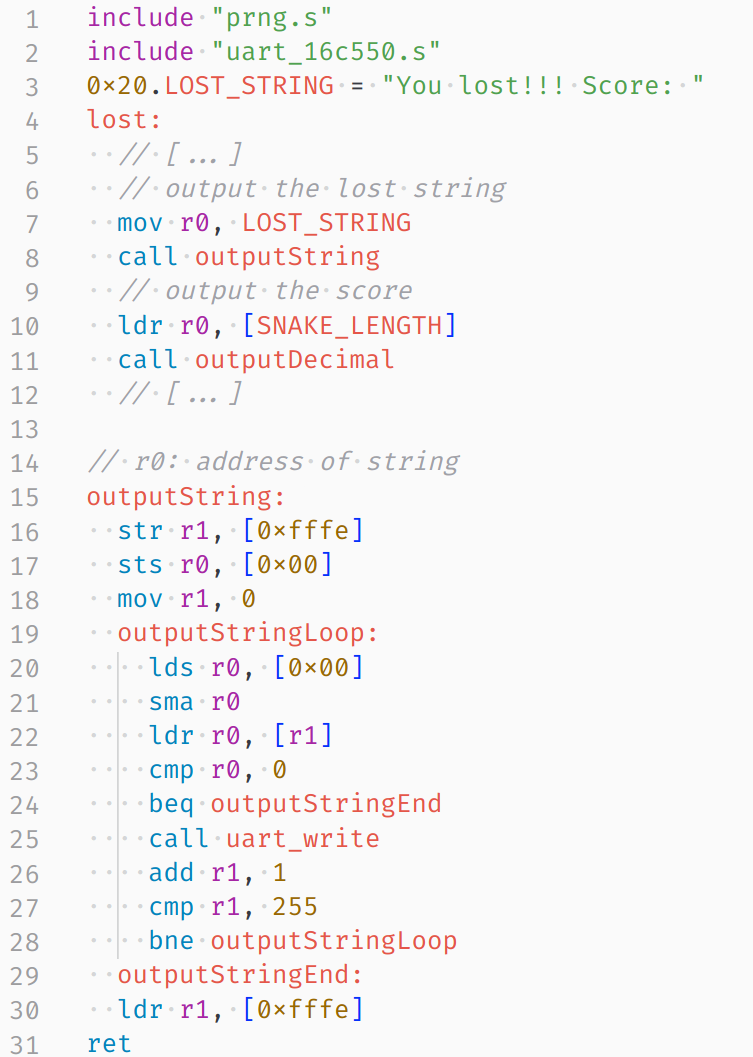
\includegraphics[width=.7\textwidth]{syntax_snake_excerpt.png}
  \caption{The syntax highlighting with the \gls{EDiC} Visual Studio Code Extension and the Atom One Light Theme \cite{VSCodeLight}.}
  \label{fig:SyntaxEDiC}
\end{figure}
Syntax Highlighting has become a very important factor for software development as \glspl{IDE} grow more capable.
The highlighting is usually done by firstly, parsing the syntax and associating parts of the text file with specific categories and, secondly, assigning styles like font color to these categories.
This way, a programmer can select a global color scheme which will define colors for different categories for all programming languages.
When applied correctly, code in different languages becomes easier to recognize because variables are always colored the same way, no matter the language.
The syntax parser, however, needs to be selected correctly for each file type and categorize the file content correctly.

Even though the \gls{EDiC} syntax is similar to the ARM syntax, it is not syntactically identical which makes syntax highlighting in editors difficult.
As can be seen in \cref{lst:asm_snake_excerpt} line 3, the ARM syntax definition used for the highlighting in this document is not perfect (The leading 0 is red, and the string is not colored correctly).

As Visual Studio Code \cite{VSCode} is one of the leading extensible code editors, an extension for \gls{EDiC} assembler has been developed and published \cite{VSCodeEDiC}.
The code of the \cref{lst:asm_snake_excerpt} is shown again in \cref{fig:SyntaxEDiC} as it is highlighting using the developed extension.
The extension itself mainly consists of a TextMate language definition \cite{TextMate} and configuration files to work correctly with Visual Studio Code.
TextMate is a tokenization engine which works with a structured collection of regular expressions as language definitions.
% !TeX root = ../thesis.tex
\chapter{\glsxtrshort{FPGA} Model}\label{cha:fpga}
The goal of the \gls{FPGA} model is to proof the general workings of the \gls{CPU} architecture before finalizing the hardware layout and \gls{PCB} design.
With the design running on an actual \gls{FPGA} it is also possible to debug and test extension cards without the actual hardware of the \gls{EDiC}.


\section{\glsxtrshort{FPGA} Background}
An \gls{FPGA} can be seen as an intermediary between \glspl{ASIC} and general purpose \glspl{CPU}.
It allows for a lot more design flexibility in contrast to \glspl{ASIC} by being reprogrammable but at the same time has similar applications.
The first \gls{FPGA} was released by Altera in 1984 which featured a quartz window to erase the \gls{EPROM} cells that hold the configuration.
It only had eight macrocells and a maximum frequency of about 30MHz \cite{ref:altera_databook}.
Today's \glspl{FPGA} can have several million logic elements with several hundred MBs of \gls{BRAM}, more than a thousand floating-point \glspl{DSP} and usual frequencies of more than 200MHz.
However, the general idea of how \glspl{FPGA} work stayed the same:

\emph{Field Programmable} means that the \gls{FPGA} can be programmed in the application field, even though configure is the better word to be used.\\
\emph{Gate Array} stands for an array of logic gates which make up the \gls{FPGA}.
These logic gates can then be freely routed by the developer and with that different logic functions can be implemented.

\glspl{FPGA} are built out of so-called \glspl{CLB} which can be connected with each other to create larger designs.
Such a \gls{CLB} contains several elements like \glspl{LUT}, registers and \glspl{MUX} which allows one \gls{CLB} to provide different functionality as needed.
\begin{figure}
  \centering
  \includegraphics[width=.8\textwidth]{lut.pdf}
  \caption{Internal structure of a 2-bit \gls{LUT}}
  \label{fig:lut}
\end{figure}
Each \gls{LUT} can encode any kind of multi-bit boolean functionality.
\Cref{fig:lut} shows how a 2-bit \gls{LUT} is built out of three 2-to-1 \glspl{MUX}.
Depending on the input values of the \gls{SRAM} into the \glspl{MUX}, a different logic function can be implemented.
For example: For a \texttt{NAND} function, the \gls{SRAM} is loaded with the bits \texttt{0111}.
In \glspl{FPGA} these \glspl{LUT} usually take 4-6 bit inputs and can, therefore, implement more complex logic functions.

Combining these \glspl{LUT} with registers, complex hardware \glspl{DSP} and a lot more advanced hardware, modern \glspl{FPGA} are very capable and complex devices that are increasingly used in prototyping and low to medium quantity products.
There are several cheaply available \glspl{FPGA} development boards that are very well suited for a \gls{FPGA} prototype of the \gls{EDiC}.

\section{\glsxtrshort{FPGA} Choices}
For the \gls{EDiC} the Nexys A7 development board \cite{nexysA7} with the AMD-Xilinx Artix 7 XC7A100T-1CSG324C \gls{FPGA} has been chosen.
Its synthesis tool is the AMD-Xilinx Vivado \cite{vivado} which is available as a free version and includes an advanced simulation environment.

\subsection{Language Choice}
There are two main \glspl{HDL}: Verilog and \gls{VHDL}.
Both are widely supported and can also be used in the same project with the help of mixed-language compilation.
At the \gls{TUB} \gls{VHDL} is taught, however, in general both are used about equally often \cite{vhdlVerilog}.
As Verilog is often cited as being less verbose and, therefore, easier to write and understand it was chosen as the hardware description language.

\begin{listing}
  \inputminted[linenos,
    breaklines,
    firstline=65,
    lastline=71,
    frame=leftline,
    xleftmargin=20pt,
  ]{verilog}{src/alu.v}
  \caption{Behavioral Verilog Description of the Adder (including XOR and AND) of the \gls{ALU} module.}
  \label{lst:alu}
\end{listing}
\Cref{lst:alu} shows the Adder described in Verilog as an example.
It iterates over all 8 bits, calculates the XOR and AND results and based on these and the carry input, the bit result and the carry output is calculated.

\subsection{Tri-state Logic in \glsxtrshortpl{FPGA}}
One major problem with tri-state bus logic for \glspl{FPGA} is that most current era \glspl{FPGA} do not feature tri-state bus drivers in the logic slices.
Most \glspl{FPGA} do have bidirectional tri-state transceiver for \gls{IO} but not for internal logic routing.
However, the \glspl{HDL} (both \gls{VHDL} and Verilog) support tri-state logic and the AMD-Xilinx Simulation tool also does.
Therefore, a simulation with tri-state logic would work, but it cannot be synthesized.

\begin{sidewaysfigure}[ph]
  \centering
  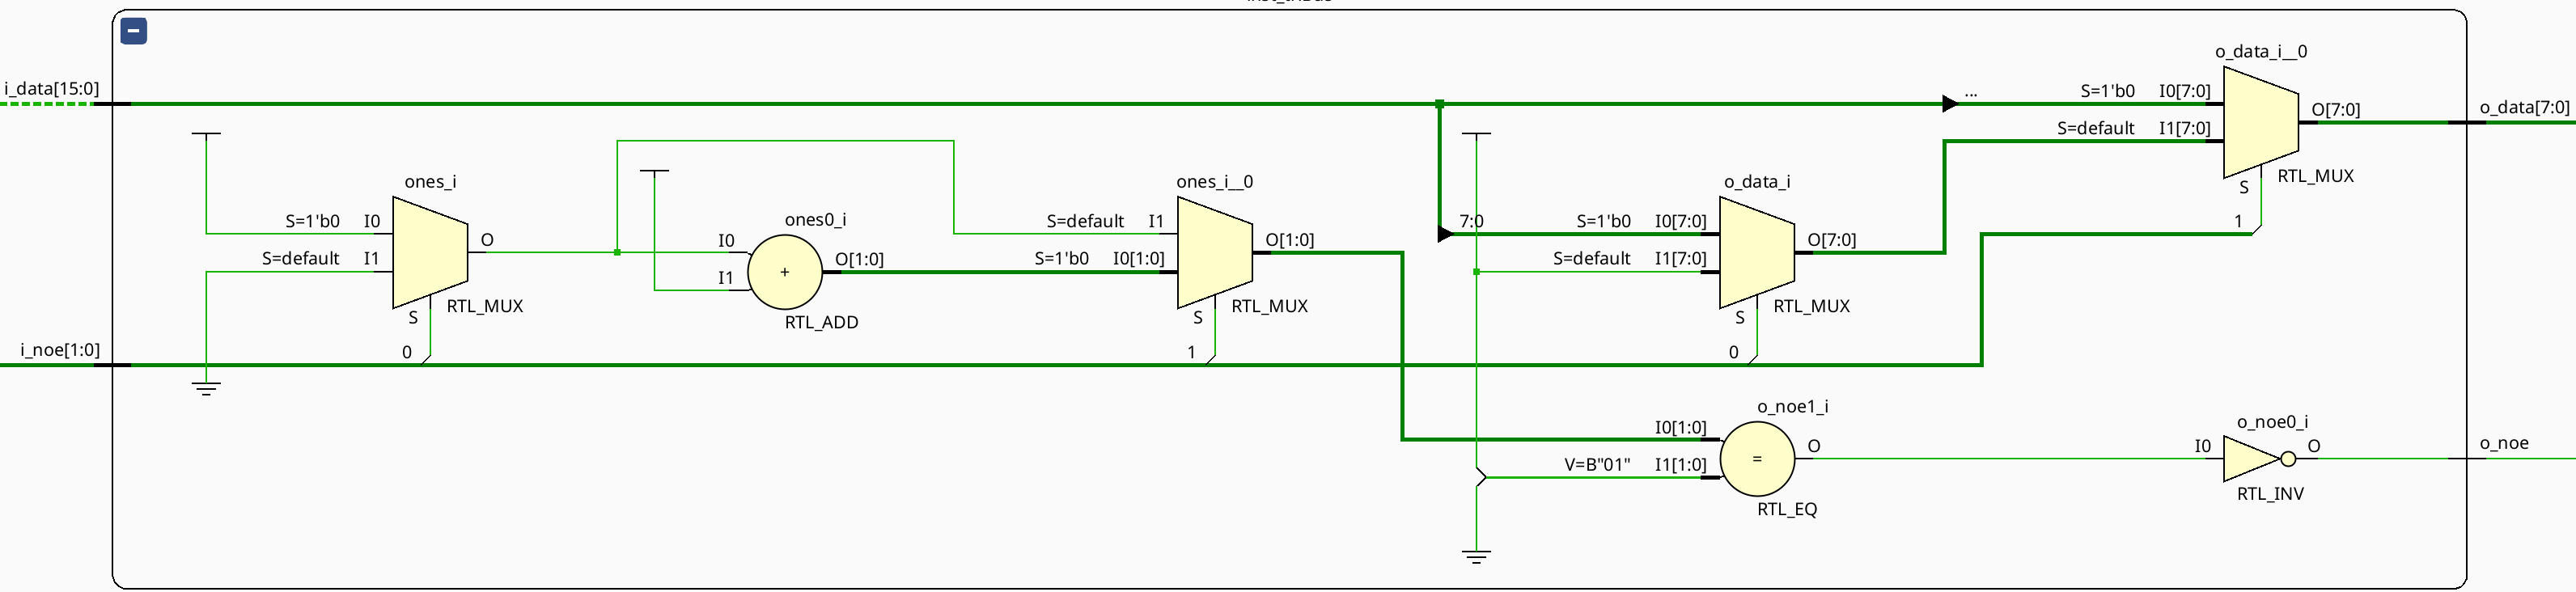
\includegraphics[width=\textwidth]{tristatenet.png}
  \caption{The elaborated tri-state module with two 8 bit inputs.}
  \label{fig:tristatenet}
\end{sidewaysfigure}
This is solved with a custom module for each tri-state network ``tristatenet.v''.
Each tri-state driver exposes the current data and output enable signal to the tri-state module which then has only one output which represents the value of the net.
If none of the drivers have an active output enable, the output is \texttt{0xff}; if one of the drivers has an active output enable, the output represents its value.
Furthermore, if more than one driver has an active output enable, an error is raised.
The module's logic representation for a tri-state net with two inputs is shown in \cref{fig:tristatenet}.
The output \texttt{o\_noe} is only active (low) if exactly one input \texttt{i\_noe} is active (low) and depending on it, the data output is selected.
For this \gls{FPGA} this tri-state logic module is implemented with one \texttt{LUT4} primitive per output data bit.

\section{Behavioral Implementation}
Two kinds of \gls{FPGA} designs were developed during the development.
The first is a behavioral description of the whole \gls{CPU} and, therefore, only models the general workings of a module but does not describe the individual chips that are used in the final hardware assembly.
The description in \cref{lst:alu}, for example, is a behavioral description as it only describes the logical level of what should happen.
This is quite useful for development, because it is quickly changed and bugs are fixed more efficiently as opposed to a chip-level model.

To visualize how a behavioral simulation looks like, a simulation of the code in \cref{lst:add_wave} is shown in \cref{fig:add_wave}.
The first instruction (\mintinline{ARM}{mov r1, 0x12}) starts at \qty{1}{\micro\second} where the instruction step counter is 0 and the instruction fetch is executed.
Step 1 increments the program counter and starts the instruction decoding.
The \mintinline{ARM}{mov} instruction only consists of one step and, therefore, the \texttt{ctrInstrFinishedN} signal is asserted in step 2 together with the control signals of the actual instruction.
Due to \texttt{ctrInstrFinishedN}, the step counter is reset to 0 and the second instruction (\texttt{pc==1}) is executed.
After the instruction fetch steps, the \gls{ALU} adds \texttt{0x12} and \texttt{0x42} at \qty{2}{\micro\second} and writes the result into \texttt{r1} at \texttt{step==3}.
The third instruction then just branches to itself, resulting in an infinite loop.
\begin{sidewaysfigure}[p]
  \centering
  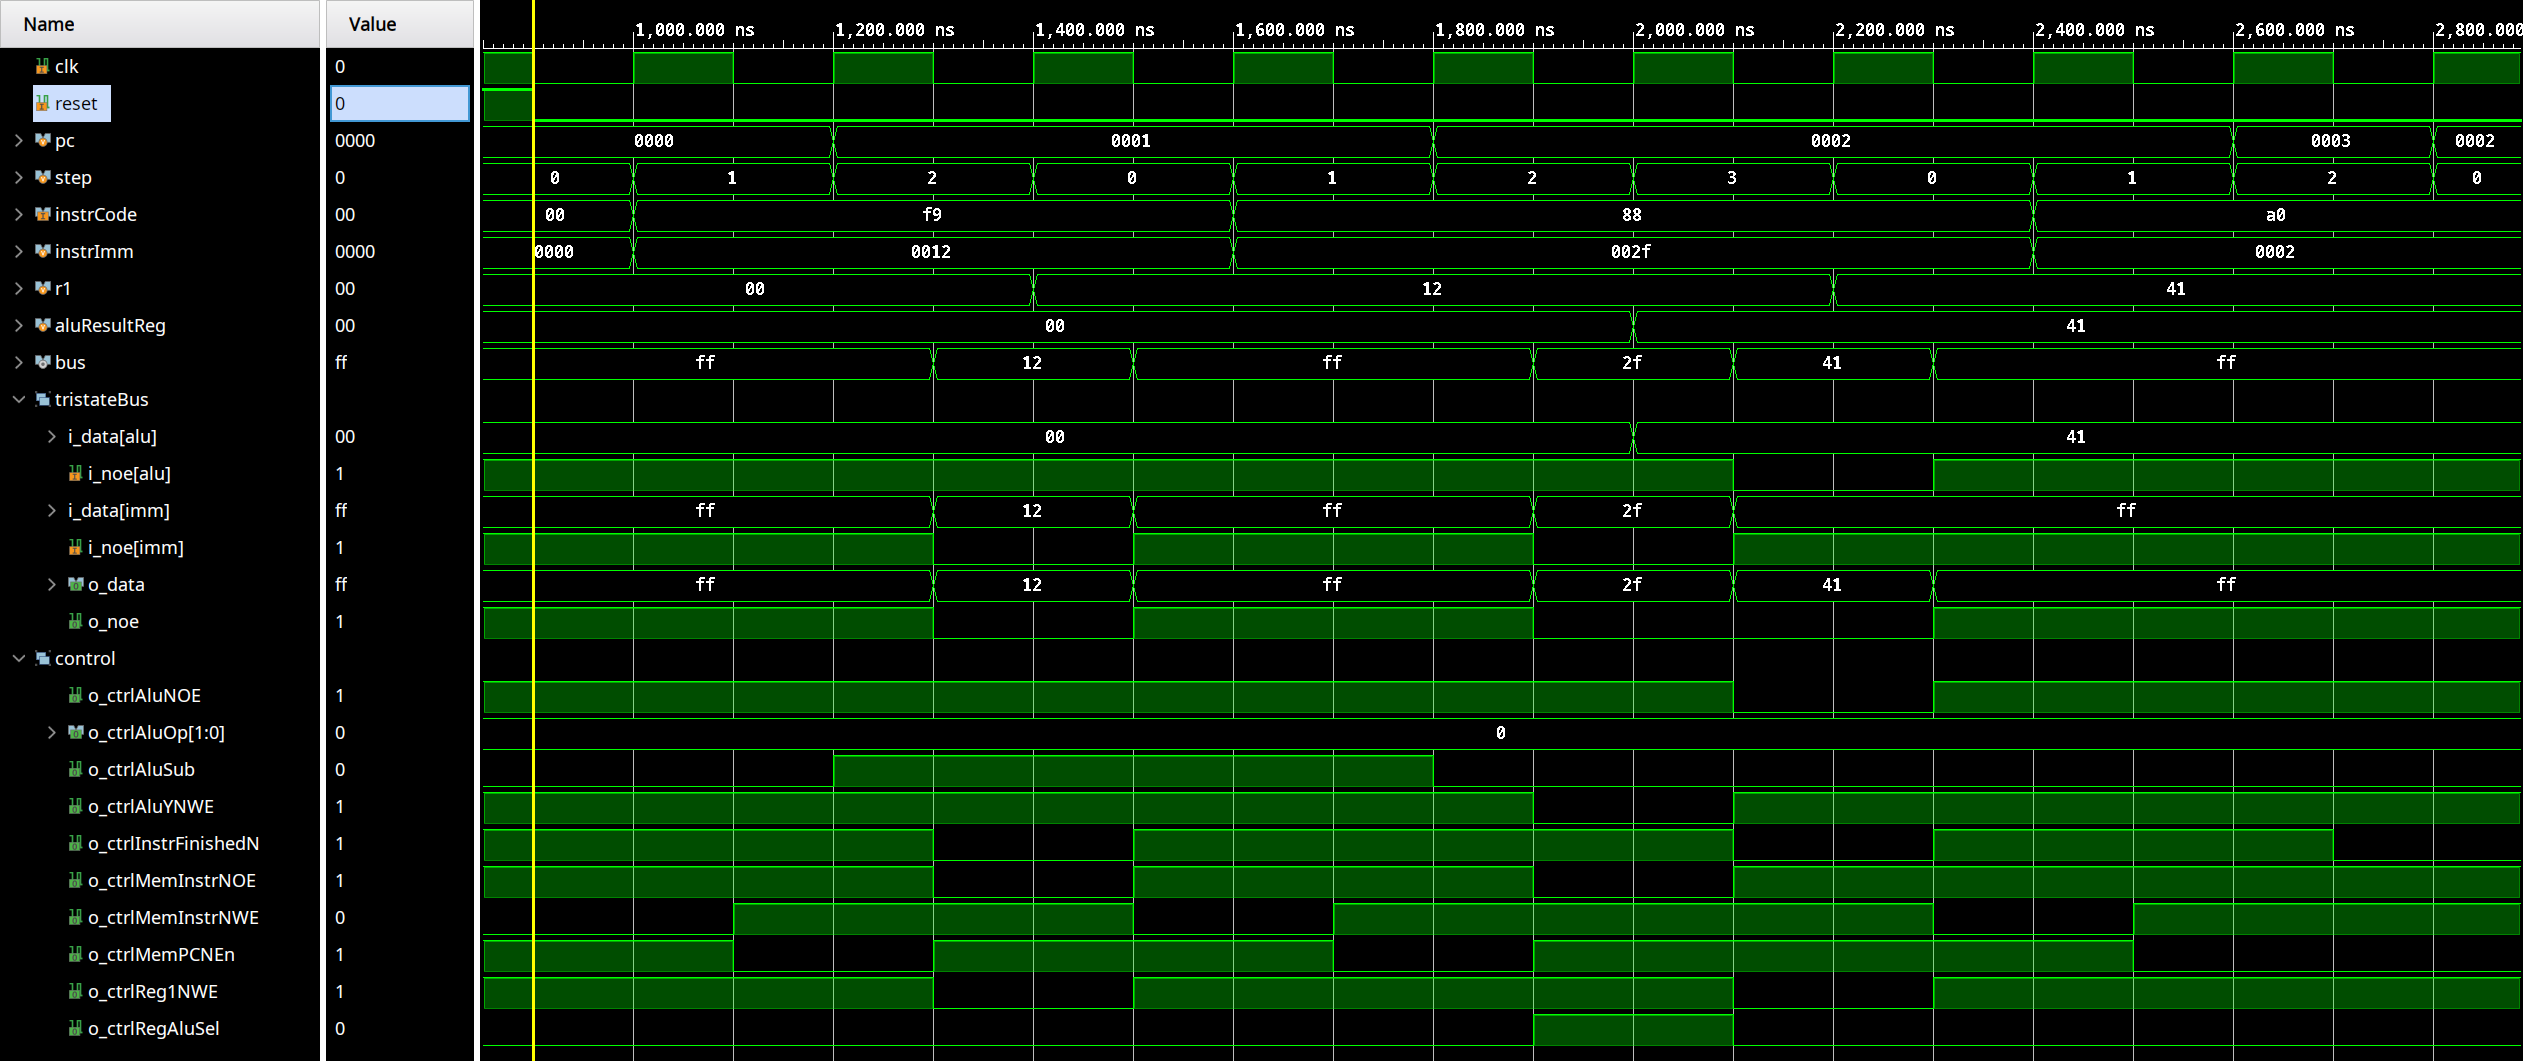
\includegraphics[width=\textwidth]{behav_add_wave.png}
  \caption{Waveform of the relevant signals for setting a register to \texttt{0x12} and adding \texttt{0x2f} to it (Assembler code is shown in \cref{lst:add_wave}).}
  \label{fig:add_wave}
\end{sidewaysfigure}
\begin{listing}
  \inputminted[linenos,
    breaklines,
    frame=leftline,
    xleftmargin=20pt,
  ]{ARM}{src/sim_test.s}
  \caption{The code for the waveform example of \cref{fig:add_wave}.}
  \label{lst:add_wave}
\end{listing}

\section{Chip-level Implementation}
With the behavioral simulation working, the hardware schematic can be developed.
The schematic as well as the placing and routing for the \gls{PCB} is described in \cref{cha:hardware}.
However, for the \gls{EDiC} it was decided to add another verification step after developing the schematic.
From the schematic a netlist is generated which is usually used to summarize all the components and connections in a machine-readable format for the software that does placing and routing.
In this case, a tool was written which converts a given netlist into a Verilog file which can be compiled and synthesized by Vivado.
\subsection{Conversation Script}
\begin{listing}
  \inputminted[linenos,
    breaklines,
    frame=leftline,
    xleftmargin=20pt,
  ]{clojure}{src/edifInstance.edn}
  \caption{An \glsxtrshort{EDIF} definition of an instance as exported by OrCAD/CAPTURE.}
  \label{lst:edifInstance}
\end{listing}
\begin{listing}
  \inputminted[linenos,
    breaklines,
    frame=leftline,
    xleftmargin=20pt,
  ]{clojure}{src/edifNet.edn}
  \caption{An \glsxtrshort{EDIF} definition of a net as exported by OrCAD/CAPTURE.}
  \label{lst:edifNet}
\end{listing}
The netlist file used is an \texttt{*.edn} which is exported by OrCAD/CAPTURE version 9.2.1.148.
It follows the \gls{EDIF} and contains a list of all instances (i.e. \glspl{IC} and other components) with port numbers and a second list of all nets (connections between ports).
The conversion script consists of a parser which analyzes such a netlist.
The parsed netlist is then further processed until a Verilog file can be created.
The generated Verilog file only consists of wire definitions and module instantiations.
Each of the instantiated modules has its own, manually written implementation.
The implementation for an \texttt{74F08} (quad AND gate) is, for example, shown in \cref{lst:74x08}.
\begin{listing}[t]
  \inputminted[linenos,
    breaklines,
    frame=leftline,
    xleftmargin=20pt,
  ]{Verilog}{src/ic74x08.v}
  \caption{Verilog implementation for the 74F08 \gls{IC}.}
  \label{lst:74x08}
\end{listing}

\Cref{lst:edifInstance} specifies the instance U54 which is an \texttt{74AS867}.
The format also specifies the port numbers, but they are not processed by the parser because they are not required.
\Cref{lst:edifNet} then specifies a net with the name \texttt{PCIN0} which connects U52 port 18 with U51 port 18 and U54 port 3.
In this case U52 and U51 are both \texttt{74F245} octal bus transceivers where port 18 is the B0 tri-state output port and U54 is a \texttt{74AS867} (synchronous up/down counter with load) where port 3 is the D0 input port.
Depending on the control signals of U51 and U52 this net connects either the 0th bit of the bus or the instruction immediate with the 0th bit of the load input of the \gls{PC}.
Internally, the list of instances and list of nets are combined into a list of instances where each instance contains a mapping of port numbers to connected nets.

The parser discards all components except logic \glspl{IC} (ID starting with `U') and \qty{0}{\ohm} resistors.
The schematic includes some \qty{0}{\ohm} resistors between control signals to be able to rewire them more easily on the \gls{PCB} if needed.
As they essentially behave as direct connections, the nets on either side of one \qty{0}{\ohm} resistor are merged.

The basic instances are easily converted to Verilog instantiations.
However, there are some obstacles that need to be taken with more advanced instances.
\subsubsection{\glsxtrshort{EEPROM}}
\begin{listing}[t]
  \inputminted[linenos,
    breaklines,
    firstline=1364,
    lastline=1368,
    frame=leftline,
    xleftmargin=20pt,
  ]{Verilog}{src/generated.v}
  \caption{Verilog instantiation of the microcode ROM generated out of three \gls{EEPROM} instantiations.}
  \label{lst:rom_inst}
\end{listing}
The six \glspl{EEPROM} (three for the instructionROM and three for the microcode) need to be instantiated with the correct data loaded into them.
Those six instantiations are identified by the unit ID and the wires are then connected to one of the custom AMD-Xilinx ROM IP Cores which are configured with the respective initial values.
The addresses for one ROM instantiation are used and then all 24 data ports from the three \glspl{EEPROM} are connected resulting in a Verilog instantiation as shown in \cref{lst:rom_inst}.
\subsubsection{Tri-state Ports}
\begin{listing}[t]
  \inputminted[linenos,
    breaklines,
    firstline=1794,
    lastline=1801,
    frame=leftline,
    xleftmargin=20pt,
  ]{Verilog}{src/generated.v}
\caption{Verilog instantiation for the tri-state Net \texttt{PCIN0}.}
  \label{lst:tristate_inst}
\end{listing}
Some \glspl{IC} provide tri-state ports.
As discussed above, they cannot be implemented on \glspl{FPGA} and, therefore, need to be converted.
The same tri-state net component as in the behavioral implementation is used.
However, for this to work, each bidirectional port of the \glspl{IC} needs to be replaced by one input and one output port.
Also, one output enable port needs to be added.
Then the output port that replaced the bidirectional port is connected to an input of the tri-state net instance and a new net is created for each tri-state net which is the actual value of the net (the output of the tri-state net module).
The tri-state net for the \texttt{PCIN0} signal (\cref{lst:edifNet}) is represented by the instantiation shown in \cref{lst:tristate_inst}.

\subsubsection{\glsxtrshort{RAM} and \glsxtrshort{EEPROM} clock}
Another problem with the \gls{FPGA} implementation in general is that both, the \gls{SRAM} and \gls{EEPROM} chips used, are asynchronous and the \gls{FPGA} only has synchronous logic elements.
In the behavioral implementation, exact timings were no requirement and, therefore, the memory and \glspl{ROM} were clocked with the inverse clock, mimicking an asynchronous behavior.
However, for the exact netlist \gls{FPGA} implementation this is not a good way to imitate the behavior.
Therefore, the exact delays of both chips were calculated with the help of the datasheets, and they are both clocked with a custom clock that is out of phase with the global logic clock by the exact amount of the delay.
\begin{figure}[t]
  \centering
  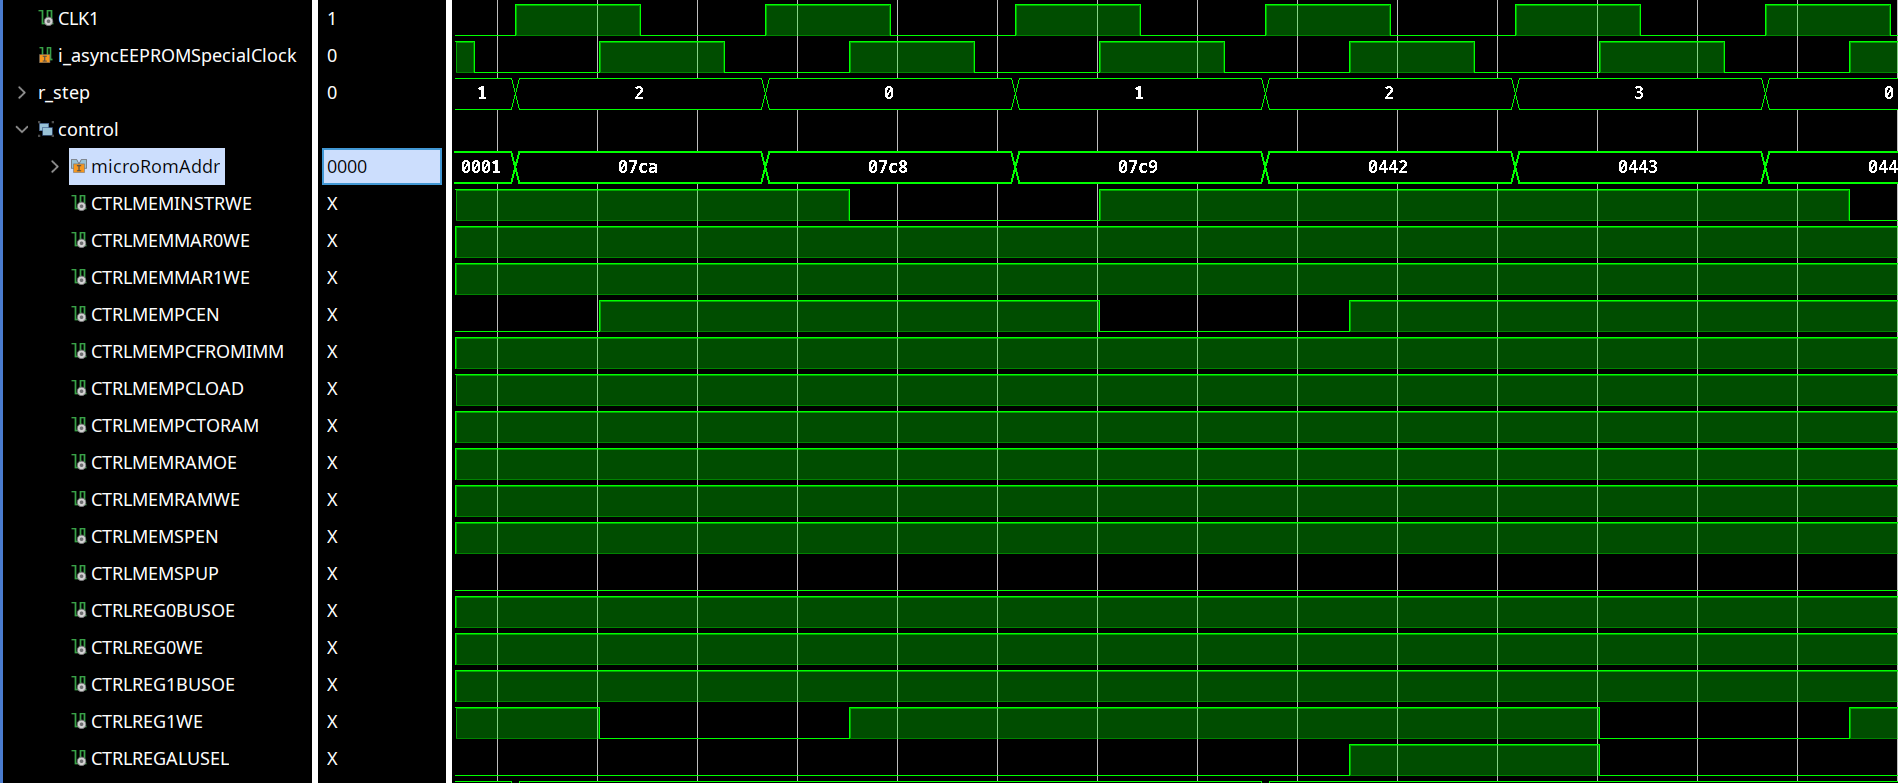
\includegraphics[width=\textwidth]{asyncClockWave.png}
  \caption{Waveform showing the clock used for the \gls{FPGA} \gls{ROM} to mimic the asynchronous behavior of the \glspl{EEPROM}.}
  \label{fig:asyncClockWave}
\end{figure}

This means, that the clock inputs of the memory and \gls{EEPROM} instantiations are replaced with the corresponding custom clock as can be seen in \cref{lst:rom_inst}.

\Cref{fig:asyncClockWave} visualizes how the main clock (\texttt{CLK1} in the waveform) and the clock for the \gls{ROM} (\texttt{asyncEEPROMSpecialClock} in the waveform) differ in phase.
Consequently, the step register and with it the address for the microcode \gls{ROM} change with a rising edge of the main clock while all the control signals which are outputs of the \gls{ROM} change with the rising edge of the phase shifted clock.

\subsubsection{Assignments}
There are some connections which are unique to the \gls{FPGA} implementation and, therefore, are not contained in the netlist.
These are mainly the inputs and outputs of the \gls{CPU} for the \gls{IO} extensions, the user buttons (reset, step etc.), clock oscillator, breakpoint addresses and so on.
However, one exception are the \texttt{L1-L4} and \texttt{H1-H4} nets which are static nets connected to ground or 5V through resistors.
They are used for logic inputs of \glspl{IC} instead of directly using GND or 5V to ease the error fixing on the \gls{PCB}.
When connected to the pane, there is no trace that can be scratched through if the pin needs to be connected to another net.
Hence, the pin usually needs to be drilled out, and the new pin needs to be insulated through the hole because it should not connect to any exposed inner layers.

In the \gls{FPGA} design the nets \texttt{L1-L4} and \texttt{H1-H4} are, therefore, assigned to 0 or 1 respectively.

\subsubsection{Display Driver}
\begin{figure}[t]
  \centering
  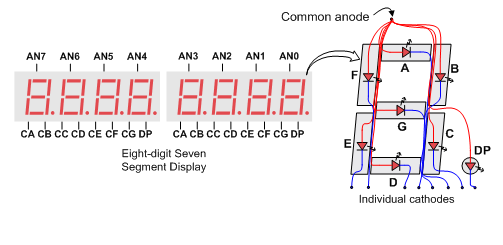
\includegraphics[width=.8\textwidth]{7segmentNexysA7.png}
  \caption{Overview of the eight 7-segment displays of the Nexys A7 development board \cite{7segNexys}.}
  \label{fig:7segNexys}
\end{figure}
The hardware build will feature two displays for the built-in \gls{IO} which can be directly addressed with 4 bits to display hexadecimal digits.
The \gls{FPGA} development board on the other hand, features simpler and more common 7-segment displays.
In total, there are eight 7-segment displays, two of which are used as the built-in \gls{IO} and the others are used for debugging when the \gls{CPU} is halted.
The wiring of the displays is shown in \cref{fig:7segNexys}.
To address these displays, a custom display driver has been developed which has eight 4 bit data inputs for the digits plus eight inputs for the dots between the digits.
Additionally, 8 bits encode which 7-segment displays should be illuminated.
It loops through the digits by setting each anode to \texttt{'0'} individually and setting the cathodes according to the corresponding input bits.
This way, each display is illuminated for \qty{2}{\milli\second} which makes it look like all displays are illuminated all the time.

\subsection{RS232 \glsxtrshort{IO} Extension Debugging}
\begin{sidewaysfigure}[p]
  \centering
  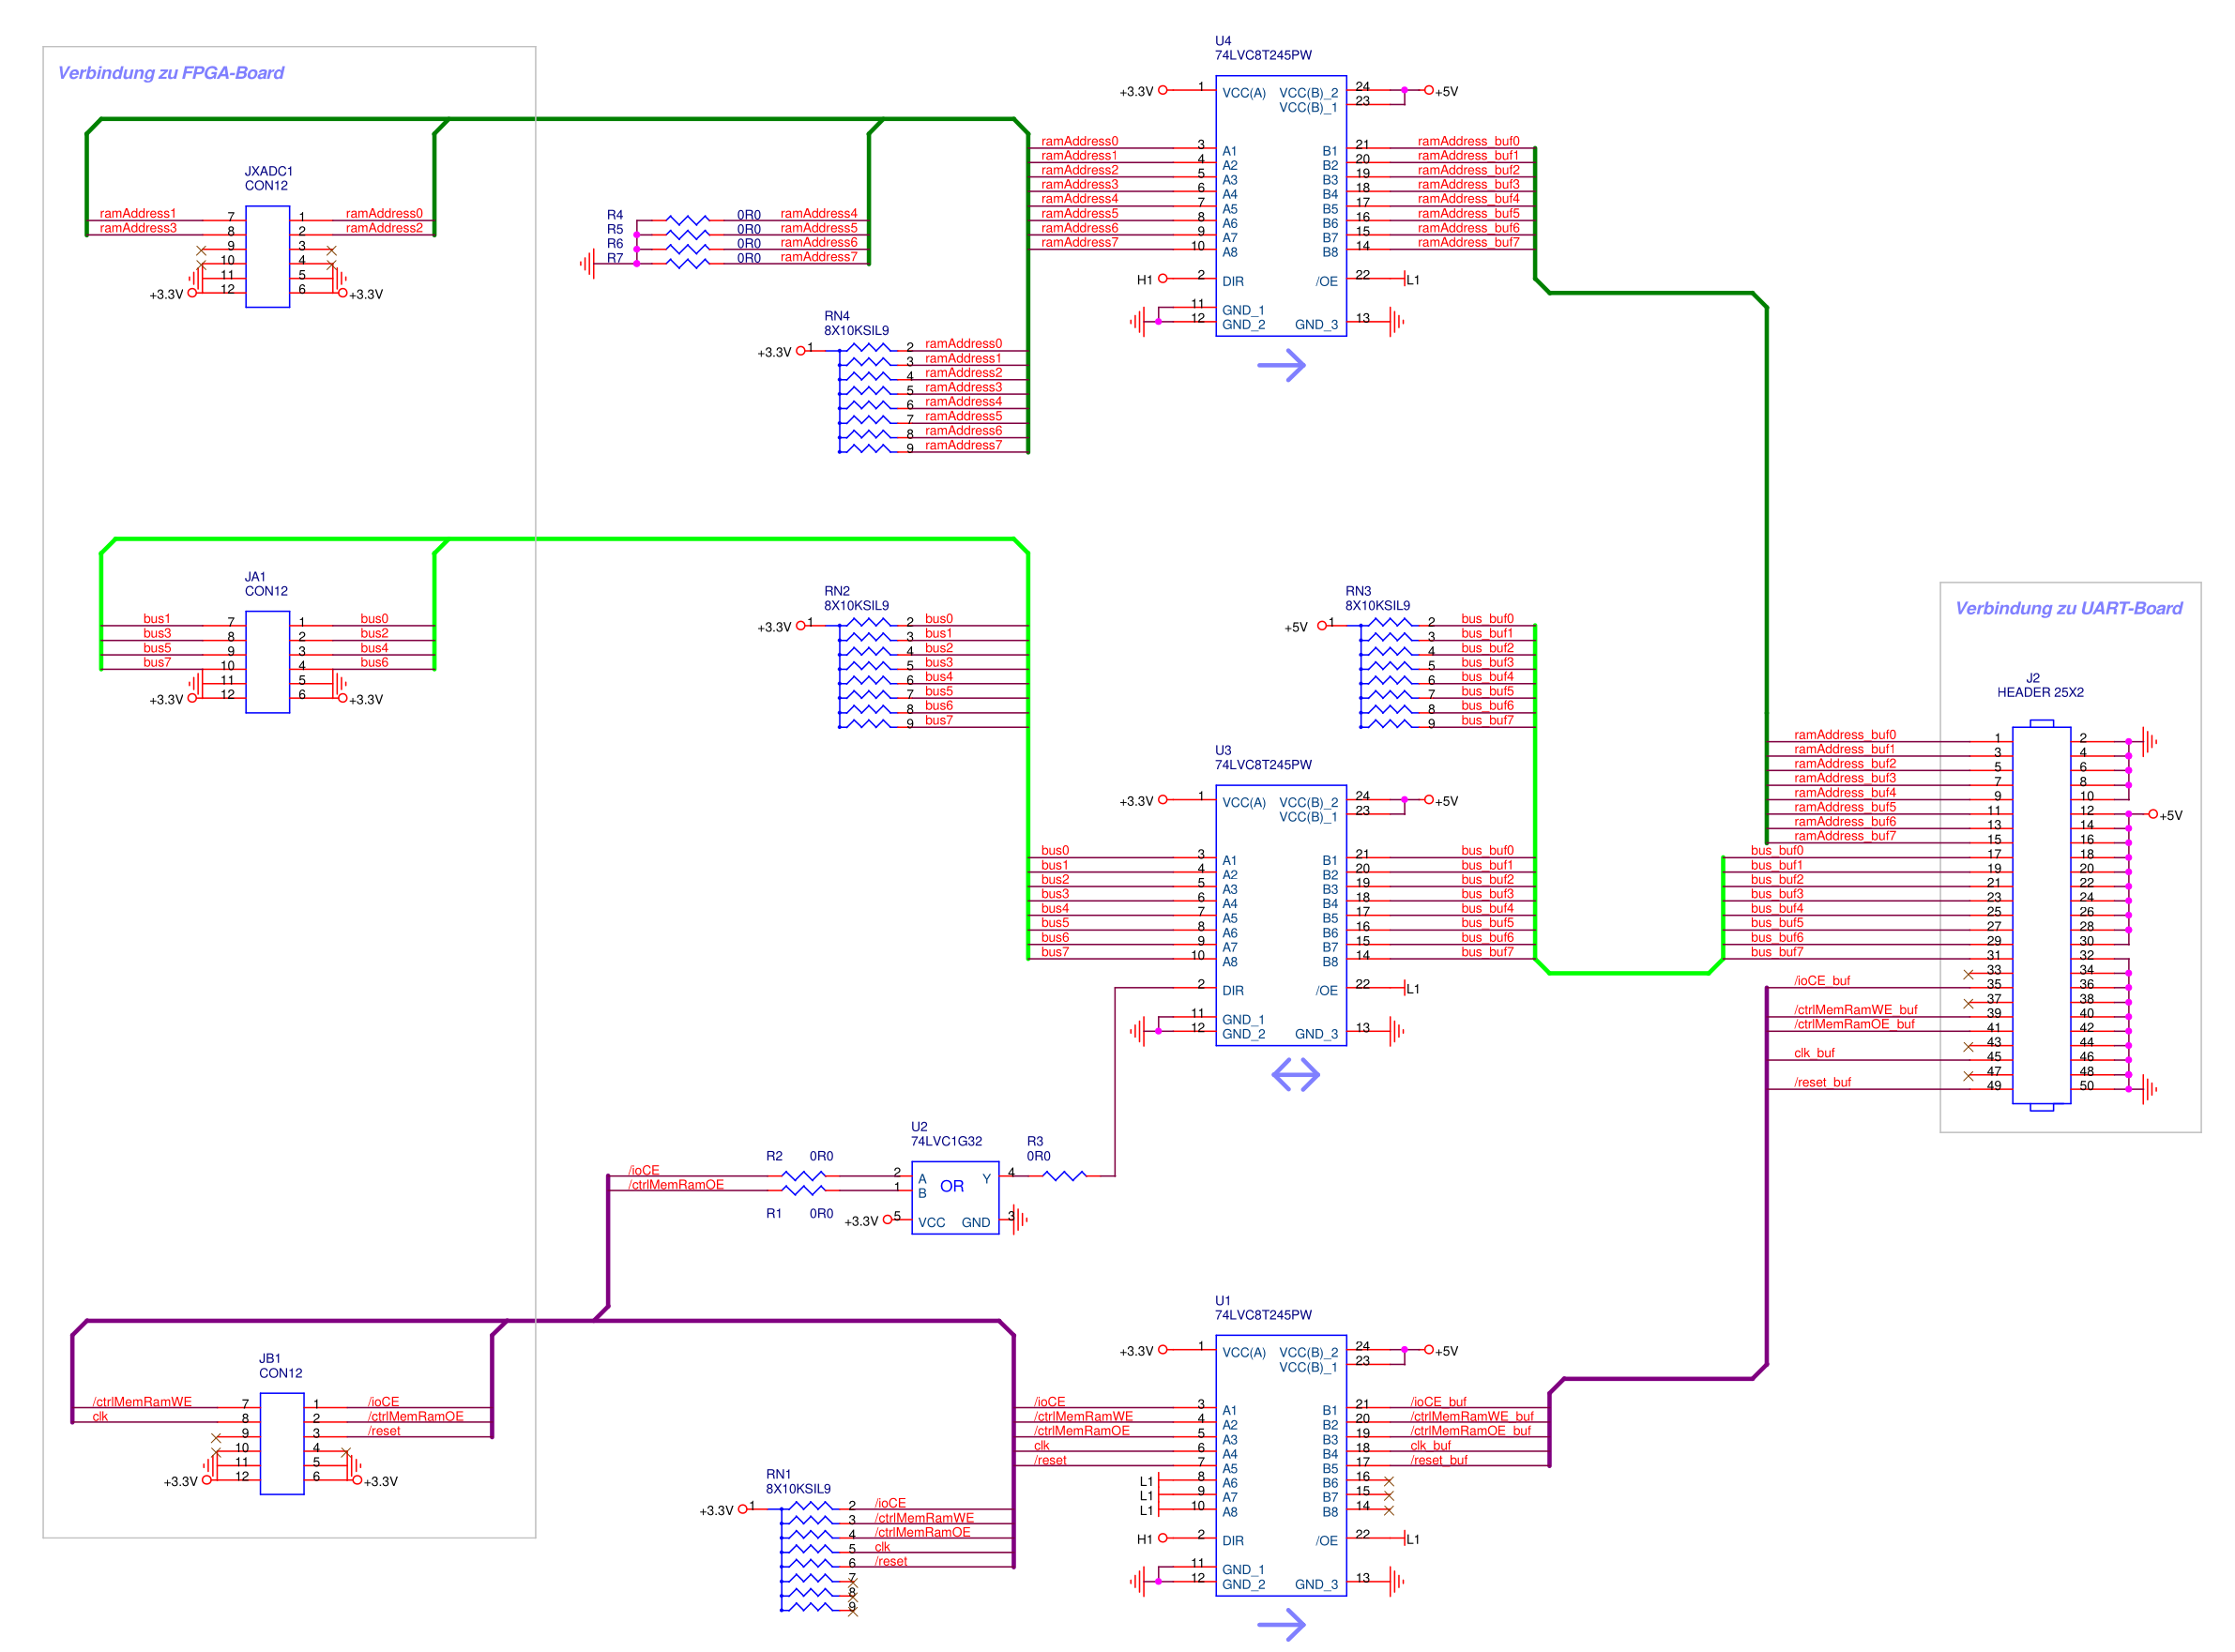
\includegraphics[width=\textwidth]{uartTestSch.png}
  \caption{The Schematic for the 3V3 to 5V conversion to use extension cards with the \gls{FPGA} development board.}
  \label{fig:3v3to5vSch}
\end{sidewaysfigure}
One goal of creating a logical replication of the \gls{CPU} on a \gls{FPGA} was to verify the \gls{IO} extension cards before ordering the large \gls{PCB} for the \gls{CPU}.
All extension cards will be daughter boards and sit on top of the main \gls{PCB} in a smaller form factor.
The following logical connections are passed through pin headers:
\begin{itemize}
  \item Bus (8 bits, bidirectional)
  \item \gls{IO} Address (lower 8 bits, to \gls{IO})
  \item Control Signals:
  \begin{itemize}
    \item \texttt{\textoverline{ioCE}}: active when the upper 8 \gls{RAM} address bits equal \texttt{0xfe}.
    \item \texttt{\textoverline{ctrlMemRamWE}}: write enable signal. Write should only happen when \texttt{\textoverline{ioCE}} is active.
    \item \texttt{\textoverline{ctrlMemRamOE}}: output enable signal. Read should only happen when \texttt{\textoverline{ioCE}} is active.
    \item \texttt{clk}: Clock signal.
    \item \texttt{\textoverline{reset}}: Reset signal.
  \end{itemize}
\end{itemize}
Additionally, ground and 5V is passed through the connector.
However, the Nexys A7 \gls{FPGA} development board only features digital 3V3 connections on the side.
Thus, an adapter board is required which converts the 3V3 voltages to 5V and the other way around while providing the correct pin locations for the Nexys A7 board and the daughter board.
Its schematic is shown in \cref{fig:3v3to5vSch} where the \texttt{74LVC8T245} is used as a voltage converting buffer.
For the control signals and addresses, its direction is always from the A port (3V3) to the B port.
The direction pin of the bus buffer, however, is low (from B to A) when both, output enable and chip enable, signals are active.
% !TEX root = ../thesis.tex
\chapter{Hardware Design}\label{cha:hardware}
After the \gls{FPGA} behavioral simulation is successful, the hardware design process is started.
The initial step is designing a schematic (\cref{sec:sch}) which is followed by the netlist simulation and the placing and routing of components and wires \cref{sec:pr}.
\begin{table}[h]
  \centering
  \renewcommand{\arraystretch}{1.25}
  \caption{All logic \glspl{IC} used in the \gls{EDiC}.}
  \label{tab:cpuIcs}
  \begin{tabularx}{\textwidth}{ |l|r||X| }
    \hline
    \gls{IC}   & Quantity & Function                                                             \\\hline\hline
    74F245     & 17       & Three-State Octal Bus Transceiver                                    \\\hline
    74ABT540   & 14       & Inverting Octal Buffer (\gls{LED} Driver)                            \\\hline
    74F157     & 12       & Quad 2 to 1 multiplexer                                              \\\hline
    74F825     & 10       & Octal register with Three-State, Asynchronous Clear and Clock Enable \\\hline
    74F86      & 7        & Quad XOR                                                             \\\hline
    74F08      & 7        & Quad AND                                                             \\\hline
    74F521     & 6        & 8 bit Inverting Comparator with Enable                               \\\hline
    28C256     & 6        & \gls{EEPROM} with 15 address bits                                    \\\hline
    74ACT245   & 5        & Octal Bus Transceiver used for \gls{SRAM}                            \\\hline
    74F153     & 4        & Dual 4 to 1 multiplexer                                              \\\hline
    74F32      & 4        & Quad OR                                                              \\\hline
    BERG40     & 3        & 40 pin Connector for Test-Adapter                                    \\\hline
    BERG26     & 3        & 26 pin Connector for Test-Adapter                                    \\\hline
    74F151     & 3        & 8 to 1 multiplexer                                                   \\\hline
    74AS867    & 3        & Synchronous 8 bit cascaded counter with loading                      \\\hline
    BERG10     & 2        & 10 pin Connector for Test-Adapter                                    \\\hline
    74F273     & 2        & Octal register with clear                                            \\\hline
    74F04      & 2        & Hex Inverter                                                         \\\hline
    AS6C4008   & 2        & \gls{SRAM} with 19 address bits                                      \\\hline
    5082\_7340 & 2        & hexadecimal display                                                  \\\hline
    74ACT14    & 1        & Hex Inverter with Schmitt Trigger                                    \\\hline
    DS1813-10  & 1        & Reset Generator                                                      \\\hline
    74F374     & 1        & Octal register with output enable                                    \\\hline
    74ABT245   & 1        & Bus driver used for clock and reset                                  \\\hline\hline
    Sum        & 118      & -                                                                    \\\hline
  \end{tabularx}
\end{table}

\section{Schematic}\label{sec:sch}
The full schematics of the hardware design can be found in \cref{cha:schem} in \cref{fig:schPC,fig:schRAM,fig:schMC,fig:schClk,fig:schIO,fig:schReg,fig:schAlu}.
The schematic is created in such a way that the logical connections are easy to understand.
Each \gls{IC} has its pins arranged for easy understanding and the connections have meaningful names to easier understand the logic.

The 74 series of \glspl{IC} is used for the \gls{EDiC}.
However, a lot of decisions need to be made in choosing the correct \glspl{IC} and
\subsection{Register Comparison}
\begin{figure}[t]
  \centering
  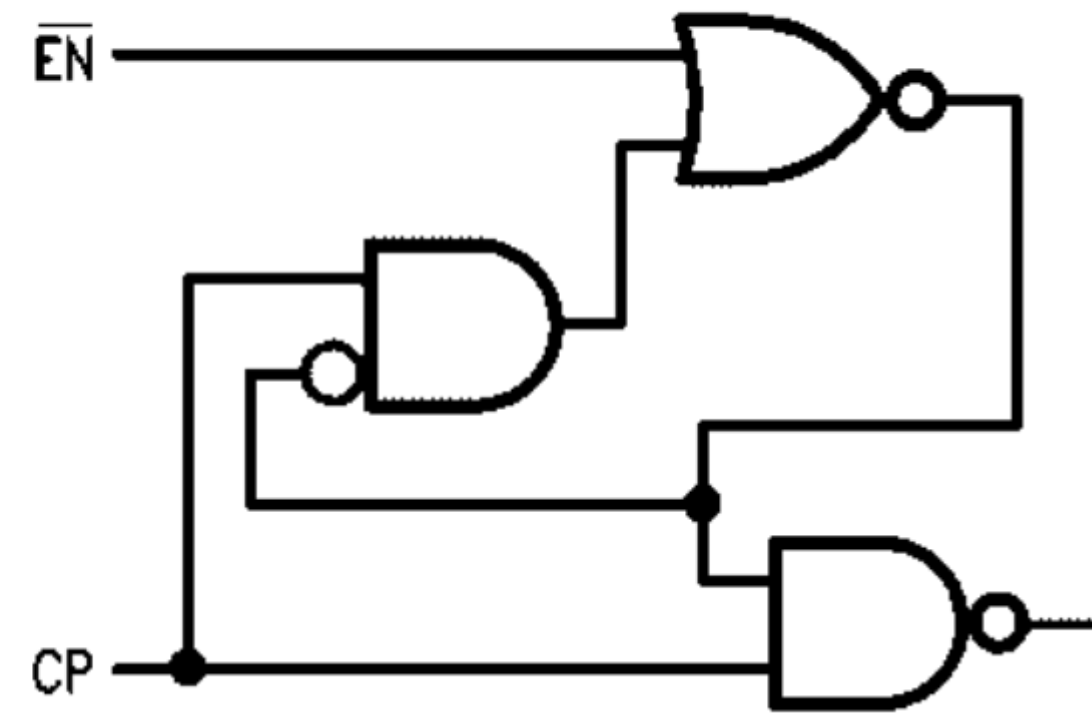
\includegraphics[width=.6\textwidth]{ce.png}
  \caption{Clock Enable circuit of the \emph{74F825} \gls{IC} \cite{74f825}.}
  \label{fig:clockEnable}
\end{figure}
The 74 series of logic \glspl{IC} feature many different registers.
The most basic register \gls{IC} has $n$ D-type flip-flops with respective data inputs and outputs plus one common clock input.
On each rising edge of the clock the flip-flops capture the input values and hold them until the next rising edge of the clock.
However, often it is required that a register does not capture data on every rising edge of the clock.
This is done with an additional input, called \emph{clock enable}.
Implementing the clock enable with a basic AND gate of the clock and a control bit has the major drawback that glitches of the enable control signal can propagate to the clock input of the register and, therefore, falsely trigger the register.
There are two widely used alternatives to the simple AND gate:
The enable input can be used as the select input for an multiplexer to the data input of the flip flop, where it multiplexes between the actual input and the current output.
This allows the flip-flop to always capture data but when the enable input is inactive, it recaptures the current output.
The drawbacks are that each bit of the register needs a multiplexer at the input and, furthermore, that the flip-flops draw power on every clock pulse, even though no new data is captured.
The \emph{74F825} logic \gls{IC} solves this with the circuit shown in \cref{fig:clockEnable}.
When the $\overline{\text{EN}}$ input is low, the CP input is NAND gate on the right passed the negated CP through\footnote{The internal flip-flops of the \emph{74F825} are negative edge triggered}.
When the $\overline{\text{EN}}$ input is high, on the other hand, the output does not change.
This circuit prevents the $\overline{\text{EN}}$ to trigger a falling edge (which would trigger the flip-flops) on the CP output.
However, when the $\overline{\text{EN}}$ goes high while the CP input is high, then the output also goes high.
This is not directly a problem because the flip-flops only trigger on falling edges but is the reason for timing requirements on the $\overline{\text{EN}}$ input which are discussed in more detail in \cref{sec:timing}.
\begin{figure}[t]
  \centering
  \begin{subfigure}[b]{.45\textwidth}
    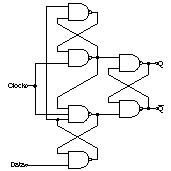
\includegraphics[height=7.5cm]{DFlipFlop.pdf}
    \subcaption{Classical D-type flip-flop built out of three $\overline{\text{SR}}$ NAND latches \cite{DFlipFlop}.}
  \end{subfigure}%
  \hspace{.05\textwidth}
  \begin{subfigure}[b]{.45\textwidth}
    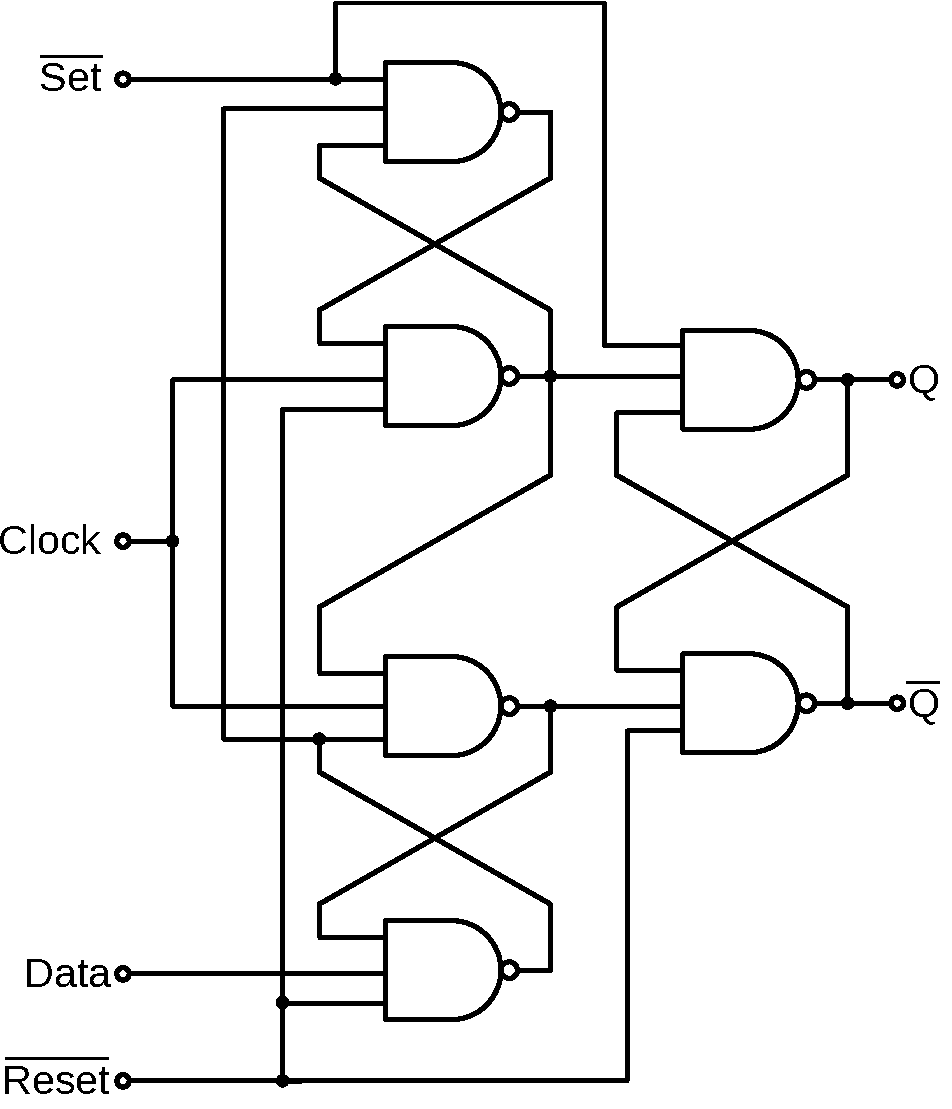
\includegraphics[height=7.5cm]{DFlipFlopClearSet.pdf}
    \subcaption{D-type flip-flop modified to support $\overline{\text{Clear}}$ and $\overline{\text{Set}}$ \cite{DFlipFlopClearSet}.}
  \end{subfigure}
  \caption{Comparison of D-type flip-flops with and without $\overline{\text{Clear}}$ and $\overline{\text{Set}}$.}
  \label{fig:clearSet}
\end{figure}

As the registers store the current state of execution, it is required that the registers start up to a known state.
Therefore, some registers feature an asynchronous clear input (or set input) which forces all flip-flops to 0 (or 1).
This is usually accomplished by modifying the classical D-type flip-flop to allow for setting and resetting the internal $\overline{\text{SR}}$ NAND latches as shown in \cref{fig:clearSet}.

A third feature that may be important is a three-state output which allows the register to be directly connected to a bus.
It is accomplished by adding a tri-state output driver to the outputs of the flip-flops.

The register that was chosen for the \gls{EDiC} is the \emph{74F825} because it has all three features and is 8 bits wide.
However, three other kinds of registers are also sparsely used in the \gls{EDiC}:
\begin{itemize}
  \item The \emph{74AS867} is a more advanced synchronous counter register which is used for the \gls{PC} and \gls{SP}. It is described below.
  \item The \emph{74F374} register only features the output enable and is used once where no additional control logic is required.
  \item The \emph{74F273} is used for the built-in I/O to mimic the typical asynchronous extension cards and for the buffering of user control inputs (stepping etc.).
\end{itemize}

\subsection{LED Driver}\label{sec:ledBuffer}
The \gls{EDiC} features many \glspl{LED} showing the register contents to aid the understanding of the workings of a \gls{CPU}.
However, naively connecting the \glspl{LED} to the logic outputs of registers may lead to unwanted behavior because the outputs of all logic \glspl{IC} have a limited current they can provide.
This leads to the usage of specific buffers for the \glspl{LED}.
Additionally, the current rating usually is higher for low-level output due to the internal workings of the output buffer as explained in \cref{sec:outputBuffer}.
For example, the \emph{74F245} non-inverting buffers B output is rated for maximum \qty{-15}{\milli\ampere} for high-level output and \qty{64}{\milli\ampere} for a low-level output \cite{74f245}.
Therefore, connecting the anode of a \gls{LED} via a current limiting resistor to the output of a non-inverting buffer and the cathode to GND will not be ideal.
To be able to draw more current from the buffer and thus having brighter \glspl{LED} inverting buffers are used and the \glspl{LED} are connected ``backwards''.
The \emph{74ABT540} is the \gls{IC} used as \gls{LED} buffer in the \gls{EDiC} with the a low-level current rating of \qty{64}{\milli\ampere} \cite{74abt540}.
The cathodes of the \glspl{LED} are then connected to the \emph{74ABT540} and the anodes are connected through current limiting resistors to $V_{cc}$.

\subsection{Program Counter \& Instruction \glspl{EEPROM}}
\Cref{fig:schPC} contains the \gls{PC} (U54 and U55) with the instruction \glspl{EEPROM} (U62, U67, U69) and the registers to store the instruction.
The \gls{PC} can be incremented or loaded from either an instruction immediate (U50 and U52) for branching or the \gls{SRAM} (U49 and U51) for returning from a function call.
To facilitate these operations, the \emph{74AS867} is used which is an 8 bit synchronous counter with loading and asynchronous clear capabilities that can be cascaded with a ripple carry output.
The \gls{PC} is then used as the address to the instruction \glspl{EEPROM} and can also be saved to the \glspl{SRAM}.
As the main memory is only 8 bits wide but the \gls{PC} 16 bit wide, a second \gls{SRAM} \gls{IC} is used to store the upper bits of the \gls{PC} in the case of a function call (see \cref{sec:schMemory}).
The \gls{PC} is, additionally, used as A inputs to the \emph{74F521} (U53 and U60) comparators to detect when a breakpoint is reached.
The 8 bit comparators can be cascaded via the enable input to compare 16 bit values.
The B input is selected by the user with four hexadecimal digit switches.

The function of the ``Test'' block between the output of the instruction \glspl{EEPROM} and the the instruction registers is explained in \cref{sec:testAdapter}.
For understanding the function of the schematic, it can be assumed that it shorts the connections on the left with the corresponding connections on the right.
The lowest of the 3 instruction registers (U64) holds the instruction code which is used in the \cref{sec:schControl}.
The upper two registers (U70 and U71) hold the immediate value which can be used as an address in the \cref{sec:schMemory}, as a branch address for the \gls{PC} and the lower 8 bits can be used as immediate value on the bus (U75).

All 5 registers have \glspl{LED} connected to them as described in \cref{sec:ledBuffer}.
\subsection{Memory}\label{sec:schMemory}
The memory module (\cref{fig:schRAM}) features three registers used for the address logic:
The \gls{MAR} (U68 and U63) is a 16 bit register where the lower and upper 8 bits can be loaded independently from the bus.
The \gls{SP} (U56) is a \emph{74AS867} counter register as the \gls{PC} but only 8 bits wide and wired differently to only allow incrementing and decrementing.
The three different kinds of memory accesses are decoded from the upper 8 address bits which either come from the instruction immediate (U74) or the \gls{MAR} (U73):
\begin{itemize}
  \item \emph{I/O access:} When the upper 8 bits equal \texttt{0xfe} (U79), the I/O \gls{CE} signal is asserted and the \gls{SRAM} \gls{CE} is deasserted.
  \item \emph{Stack access:} When the upper 8 bits equal \texttt{0xff} (U76), the stack memory is selected.
        Then the upper 8 bits of the address is replaced by the \gls{SP} and a 17th address bit is asserted to access the stack memory.
\end{itemize}
The address is then driven by several bus driver according to the decoding logic (U61, U63, U65, U66 and U72).

The actual \gls{SRAM} \glspl{IC} (U77 and U100) have voltage levels which are not quite compatible with the standard \emph{74F} \glspl{IC} \cite{AS6C4008} which is why all the signals connecting to them are buffered with the \emph{74ACT245} \cite{74act245} (U201, U202, U203, U204 and U205).

\subsection{Control Logic}\label{sec:schControl}
\Cref{fig:schMC} contains two registers for the address of the microcode \glspl{EEPROM} (U85, U86 and U87) of which the data pins are the control signals (\cref{sec:controlSignals}).
The first registers (U83) is used as a synchronous 3 bit step counter which increments each cycle except when the halt signal is asserted.
The instruction finished control signal will reset the step counter to 0 at the next cycle.
U83 also registers the four \gls{ALU} flags and U84 registers the instruction to synchronies all address bits for the \glspl{EEPROM}.

\subsection{Clock and Reset}\label{sec:schClock}
\Cref{fig:schClk} contains the oscillator (X1) which frequency is determined in \cref{sec:timing} and a active low reset controller (U34) which resets on power-on and can be combined with a user reset switch (SW1301).
The clock and reset is buffered with an \emph{74ABT245} for minimal latency.
To avoid glitches (see \cref{sec:switchGlitch}) on the four user inputs, a low pass and a Schmitt trigger and two registers are used.
A multiplexer (U39) generates the halt signal from the debug user inputs and the instruction finished control signal to implement the logic described in \cref{sec:clock}

\subsection{Built-In I/O}
The built-in I/O (\cref{fig:schIO}) consists of one register to hold the output value (U92) which is connected to two hexadecimal displays (U93 and U94).
For input two hexadecimal switches (SW10 and SW11) are used with a bus driver (U91).
To control the register clock pulse and the output enable of the bus driver, the I/O \gls{CE} is combined with the I/O write enable and I/O output enable and the I/O address is compared with \texttt{0x00} (U88).

\subsection{Register Set and \gls{ALU} output}
The register set in \cref{fig:schReg} consists of two registers (U40 and U41) which can be loaded from the bus.
The register outputs can drive the bus (U44 and U45) and are multiplexed for the A input of the \gls{ALU} (U42 and U43).
After the combinatorial \gls{ALU} (\cref{sec:schALU}), the four operation results are multiplexed (U5, U6, U7 and U8) and stored in the \gls{ALU} output register (U9).
Even though the \gls{ALU} output register features output enable inputs, an indivual bus driver is used (U10) because the content of the \gls{ALU} output register should be displayed to the user (U11).
The carry flags are also multiplexed (U101) as the carry flag from the shift operation is generated independently.
The overflow flag is generated in the combinatorial schematic of the \gls{ALU}, the negative flag is just the \gls{MSB} of the output and the zero flag is deduced from a comparison with zero (U12).
All four flags are then stored in a register (U97).
\subsection{Combinatorial \gls{ALU}}\label{sec:schALU}
\Cref{fig:schAlu} shows the ripple carry adder on the left composed out of 8 full adder and with subtracting capabilities.
The barrel shifter on the right side is explained in depth in \cref{sec:alu}.
The carry flag resulting from a shift operation should always represent the last bit which was shifted out of the 8 bits and should be unchanged when shifting by 0.
This is accomplished with another multiplexer (U102).

\section{Placing and Routing}\label{sec:pr}
\begin{figure}[p]
  \centering
  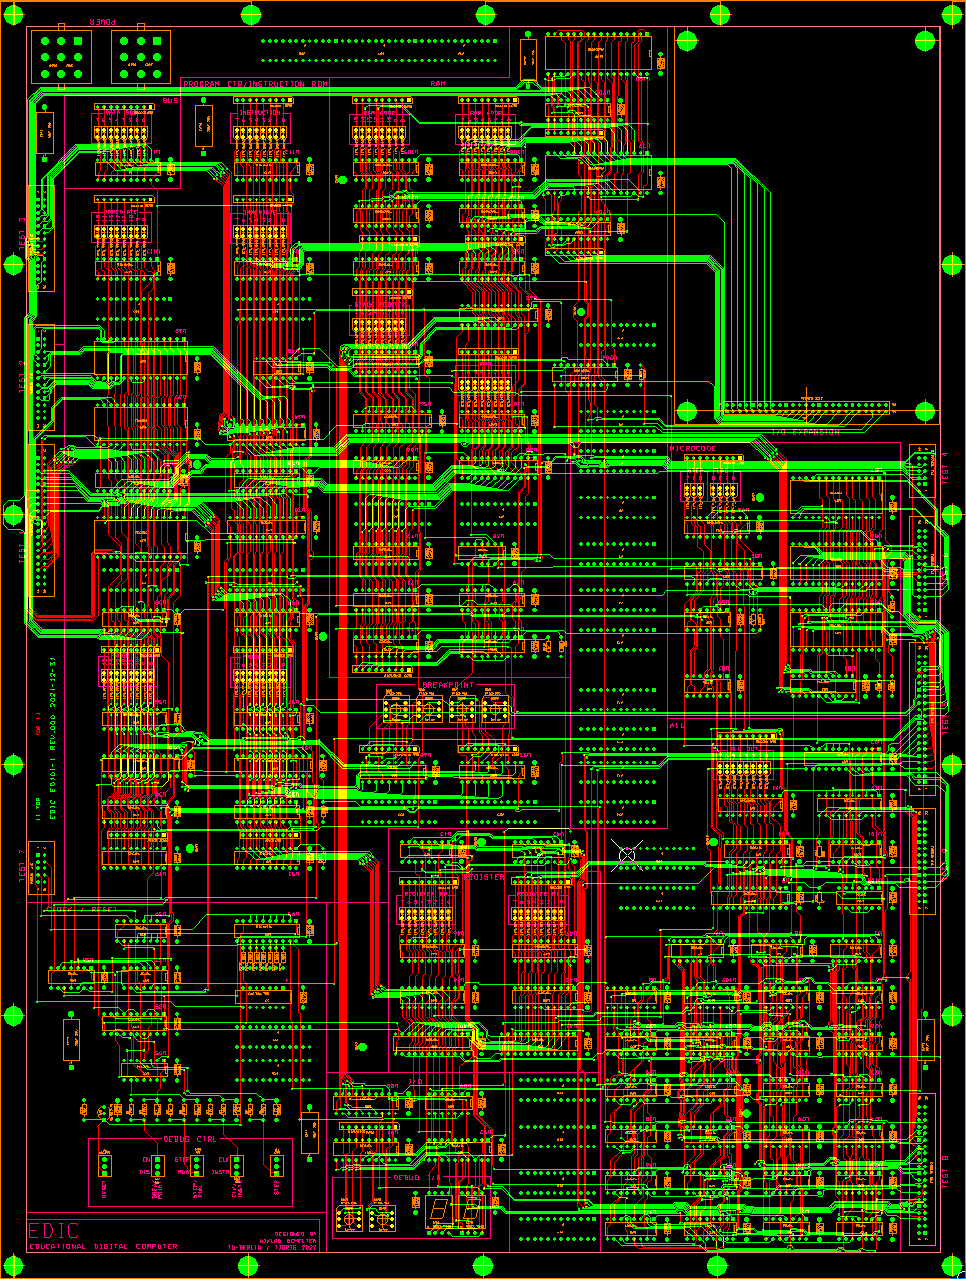
\includegraphics[width=\textwidth]{PR.png}
  \caption{Rendering with all components placed and all the traces routed on the two logic layers (green and red).}
  \label{fig:pr}
\end{figure}
For placing and routing several factors are important.
As the goal of the \gls{EDiC} is to be easy to understand for future students, all components were not only placed to optimize the wiring but also to place components of the same modules close together.
Additionally, extra space was left to mark each module and to name all the \glspl{LED} on the silkscreen of the \gls{PCB} for easier reference.
\Cref{fig:pr} is a rendering showing the traces (red and green), silkscreen (violet) and through-holes/vias (green/yellow).

Especially on larger \glspl{PCB} and designs with quickly switching power consumption it is important to ensure good power delivery to all components.
In the case of the \gls{EDiC} this is achieved by using a 4-layer \gls{PCB} with the two internals layers being filled with GND and 5V panes.
The top and bottom layer are then used for logical connections where the most efficient wiring can be done when one layer mostly has vertical wires (red traces in \cref{fig:pr}) and the other layer mostly horizontal wires (green traces).
This way interference of vertical and horizontal traces is not possible due to the GND and 5V panes separating the logic panes.

Another important factor to bear in mind is to route the traces in a way that makes it possible to access every trace.
It is always possible that some bug was not detected in the schematic design or netlist simulation.
If a bug has been found it may be required to cut a trace and rewire it (see \cref{cha:eval}).
Therefore, logical wires are always placed on the top or bottom pane and on the top pane traces will never be completely covered by \glspl{IC}.
If, for example, connecting pins 1 and 24 of a 24 pin \gls{IC} (they are directly opposite of each other) they should not be connected directly but a detour should be taken to expose the trace from under the \gls{IC}.

It is also possible that a further \gls{IC} needs to be placed on the \gls{PCB} to fix a bug, like an extra register or bus driver.
Therefore, through holes are provided to allow spare \glspl{IC} to be placed at convenient locations throughout the \gls{PCB}.

\section{Timing Analysis}\label{sec:timing}
\begin{figure}[t]
  \centering
  \includegraphics[width=\textwidth]{timingExample.pdf}
  \caption{Timing relations for a combinatorial datapath between two registers.}
  \label{fig:timingExample}
\end{figure}
To figure out what the maximum frequency is at which the \gls{EDiC} can operate on, a detailed timing analysis was performed.
The timing analysis computes the path with the longest propagation delay which called the critical path.
The delay of the critical path can then be used as a baseline for choosing the correct frequency.

\Cref{fig:timingExample} visualizes how the propagation delays work:
Each \gls{IC} has delays which are specified in the datasheet.
In the example of \cref{fig:timingExample}, a value of register $r_0$ goes through a combinatorial path and is then stored in register $r_1$.
The registers have a propagation delay $t_p$ which specifies the time from a rising edge of the clock to the output (Q).
In theory it is also important to hold the input data of a register for the specified hold delay $t_h$, however, in the \gls{EDiC} this is no problem.
Then the combinatorial path also has propagation delays from inputs to outputs which need to be added up ($t_c$).
At the next register, a setup time $t_s$ has to be met which specifies the amount of time the input data needs to be stable before the rising edge.

\begin{figure}[t]
  \centering
  \includegraphics[width=\textwidth]{all_cycles.pdf}
  \caption{Timing analysis for the control signals.}
  \label{fig:timingControl}
\end{figure}
\twopagepicture{p}{ram.pdf}{Timing analysis for the memory latency.}{fig:timingRam}
\twopagepicture{p}{alu.pdf}{Timing analysis for the \gls{ALU} latency.}{fig:timingAlu}
The \cref{fig:timingControl,fig:timingRam,fig:timingAlu} show three timing analysis for the \gls{EDiC}.
Each block represents one \gls{IC} with the corresponding delay.
The first column shows the unit number of the schematic, the second line the type of \gls{IC} and the third shows the kind of delay with the fourth showing the time.
The kind of delay of a buffer can for example be d$\rightarrow$ q which means input data to output data delay or oe$\rightarrow$ q which is the time from asserting output enable until the data is valid.
The delay time is always the worst case time as specified in the datasheet\footnote{Propagation typically varies with the temperature and age of the \gls{IC} and by taking the worst case time (maximum) it is assured that no timings bugs occur due to e.g. weather changes.}.
A vertical double line represents a point where multiple delay paths must be met until the execution can continue.
In \cref{fig:timingControl} for example, the propagation delay of register U83 (flags and step register) and register U84 (instruction) must both be over until the address for the \glspl{EEPROM} U85, U86 and U87 are valid.
At these points the maximum of the merging delay paths is used as the starting point for the next path.
The maximum delay up to this point is also added at the top.
Additionally, some paths are labeled for clarity.
All the times of the critical path (the path that takes the longest from one starting point to one end point) are marked in red.

\Cref{fig:timingControl} shows the basic latency path for control signals and the common bus driver \glspl{IC}.
The latencies inside the register set and program counter are neglectable and, therefore, only the memory module with the complex address decoding and the \gls{ALU} is further examined.
For the memory module (\cref{fig:timingRam}), there are two critical paths:
The first comes from the \texttt{memInstrToRamAddr} control signal, through the stack selection logic to the memory address and finally to the buffered output data of the \gls{SRAM} on the bus (\qty{281.3}{\nano\second}).
The second has the same origin but represents the writing option of the \gls{SRAM} (\qty{272.2}{\nano\second}).

The \gls{ALU} latency path (\cref{fig:timingAlu}) is more complex which is mainly due to the ripple carry adder.
Consequently, the critical path comes from the bus, through all the carry flags to the final adder result.
After the result multiplexer the longest path is from the zero flag to the alu flag register U97 (\qty{313.9}{\nano\second}).

Theoretically, it is possible for one instruction to read a value from the \gls{SRAM} and using it in the same instruction as an input to the \gls{ALU}.
This would replace the baseline delay of the bus input in \cref{fig:timingAlu} (\qty{169.5}{\nano\second}) with \qty{281.3}{\nano\second} and, therefore, enlarge the total worst case latency to
\begin{equation}
  \qty{281.3}{\nano\second}-\qty{169.5}{\nano\second}+\qty{313.9}{\nano\second}=\qty{425.7}{\nano\second}\label{eq:latency}
\end{equation}
Notwithstanding, because the \gls{EDiC} is a multicycle \gls{CPU} it is easily possible to assign two cycles to all \gls{ALU} operations where the B operand is read from the memory.
With this trick, the overall critical path is the maximum of \qty{313.9}{\nano\second} and half of \cref{eq:latency} which is \qty{313.9}{\nano\second}.
With a safety margin of 30\% it is feasible to choose an oscillator with a frequency of \qty{2.4}{\mega\hertz}:
\begin{equation}
  \qty{2.4}{\mega\hertz}\leq\frac{1}{1.3\cdot\qty{313.9}{\nano\second}} =\qty{2.45}{\mega\hertz}
\end{equation}


% !TEX root = ../thesis.tex
\chapter{Initial Hardware Test \& Component Verification}\label{cha:eval}
Even though the netlist was simulated and tested in the \gls{FPGA} implementation, there is no guarantee that the hardware will work out of the box.
Therefore, all bits of all components are to be tested individually to make sure there are no wiring problems which would result in bugs which are impossible to pinpoint and debug.
Testing single \glspl{IC}, especially with Three-State logic, is significantly easier when incrementally adding \glspl{IC}.
That way one driver of a Three State net can be verified and when adding another driver to the net, problems can be pinpointed to the new \gls{IC} because the first one was known to work correctly.
Therefore, all \glspl{IC} are placed inside sockets.
This way all resistors, \glspl{LED} and sockets can be soldered to the \gls{PCB} at once and all the \glspl{IC} can be placed in their sockets consecutively.
Another reason for using sockets is that it is easier to change an \gls{IC} if it is faulty or breaks in the future.
\section{Test Adapter}\label{sec:testAdapter}
To facilitate the testing, all control signals including clock and reset, the instruction register inputs and the \gls{ALU} results + flags are interrupted by connectors at the side of the \gls{PCB} which can connect to test adapter boards for testing.
For the debug signals that are not busses the test adapter has \glspl{LED} to display the state of the \gls{EDiC} and DIP Switches to set each debug signal to a known value.
Additionally, the main bus and ram2data bus is connected to a test adapter but not interrupted.
The test adapter has \glspl{LED} for displaying the state and a bus driver with DIP Switches.
If not testing, the connectors can be bridged with shorting connectors, shorting pins from the left to the right column (except the two Three-State busses).

Testing the individual components becomes very simple this way.
For example the instruction registers:
\begin{enumerate}
  \item Set each bit of the data input individually from the test adapter
  \item Assert the \texttt{memInstrNWE} control signal (set to 0)
  \item Trigger a clock pulse
  \item Verify that the output lines equal the input set on the test adapter
\end{enumerate}
All \glspl{IC}, including the \glspl{EEPROM} and \glspl{SRAM} can be directly tested in a couple simple steps this way.

The advantage of individually testing all the bits of all \glspl{IC} is that in integration testing one can assume that the problem is not with one specific \gls{IC}.
\TODO{Insert schematic of test adapter}
\section{Potential Complications}\label{sec:switchGlitch}
As is normal with large designs, there were some potential problems found in the \gls{EDiC} which needed fixing.
\subsection{Shifter - Carry Flag}
The detailed testing with the test adapter did reveal one bug which was not revealed in the netlist simulation because it did not occur.
The carry flag of a shift operation is determined by the 8 to 1 multiplexer U102 in \cref{fig:schAlu} with the first 3 bits of the bus as select bits.
The carry should always be the last bit that was shifted out of the 8 bit word.
This way, the input D1 (a0) is set as the new carry flag when shifting by 1 bit, D2 (a1) when shifting by 2 bits and so on.
However, the input D7 is connected to a7 and not a6 as it should be.
This results in a wrong carry flag when shifting by 7 bits in either direction.

In the netlist simulation this bug was not found because there was no circumstance where a value with differing bits 7 and 8 was shifted by 7 bits and the carry flag being used in the next instruction.
These kind of bugs can go undetected for a very long time and are very hard to pinpoint with a fully running \gls{CPU}.

\subsection{Clock jitter}
\begin{sidewaysfigure}[p]
  \centering
  \begin{subfigure}[b]{.45\textwidth}
    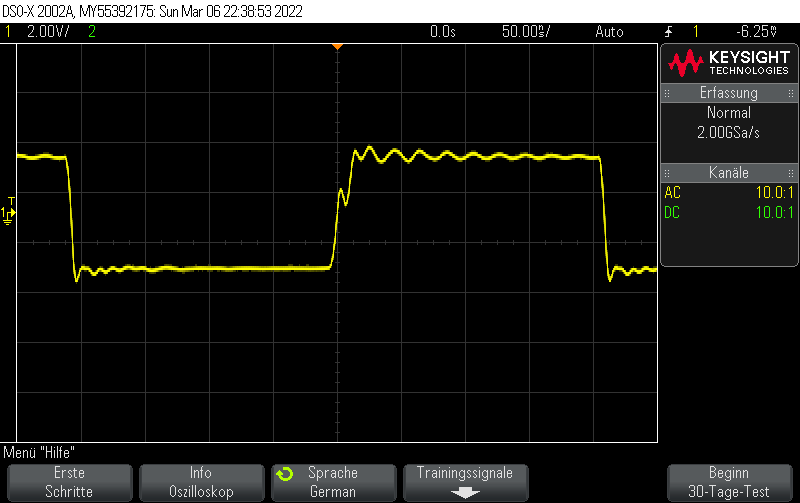
\includegraphics[width=\textwidth]{scope_0.png}
    \subcaption{No modification}
    \label{fig:clkDefault}
  \end{subfigure}%
  \hspace{.05\textwidth}
  \begin{subfigure}[b]{.45\textwidth}
    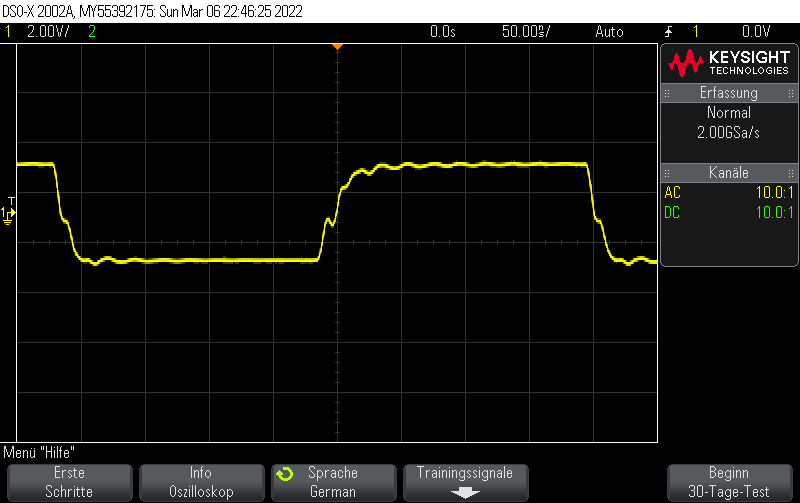
\includegraphics[width=\textwidth]{scope_2.png}
    \subcaption{R232 = \qty{33.3}{\ohm}}
    \label{fig:clk33Ohm}
  \end{subfigure}

  \begin{subfigure}[b]{.45\textwidth}
    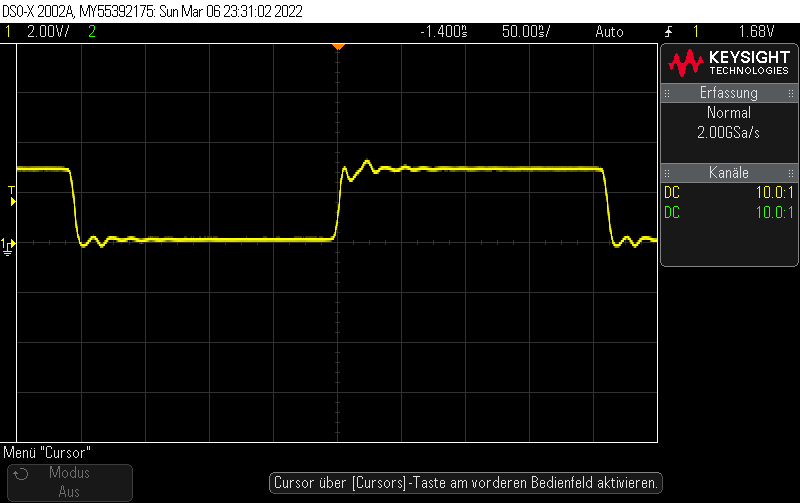
\includegraphics[width=\textwidth]{scope_3.png}
    \subcaption{R232 = \qty{0}{\ohm} and \qty{100}{\ohm} termination}
    \label{fig:clkTerm}
  \end{subfigure}%
  \hspace{.05\textwidth}
  \begin{subfigure}[b]{.45\textwidth}
    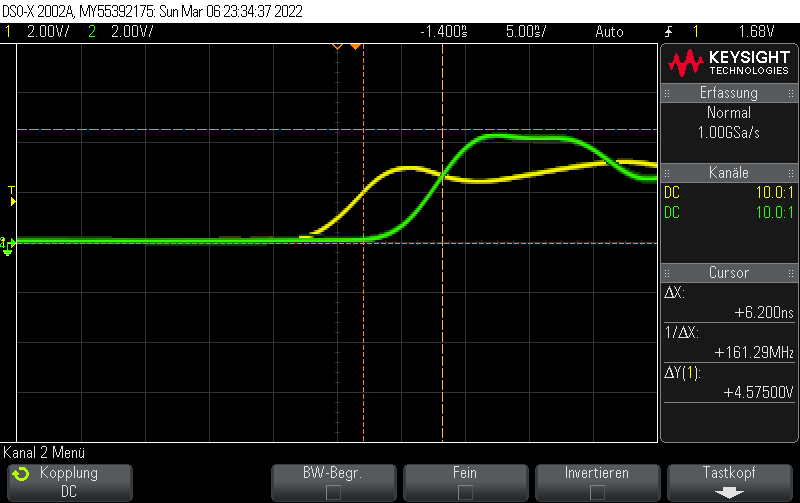
\includegraphics[width=\textwidth]{scope_7.png}
    \subcaption{Latency}
    \label{fig:clkLatency}
  \end{subfigure}
  \caption[Comparison of the clock rising edge in different configurations.]{Comparison of the rising edge of the clock in different configurations. Measured close to the clock buffer (yellow) and in \cref{fig:clkLatency} at the end of a clock lane (U204 pin 8) (green).}
\end{sidewaysfigure}
Especially with larger \glspl{PCB} a good clock distribution is a must-have.
Long clock lanes with a large load (i.e. many connected components) may induce several unwanted effects:
\begin{itemize}
  \item Jitter in the rising edge due to reflection from the ends of clock wires.
  \item A less steep rising edge due to an implicit RC-low pass filter with capacitive loads from the clock inputs and wire resistor.
  \item Over and undershoot after the edges exceeding the maximum rated voltage.
  \item Clock latency between \glspl{IC}
\end{itemize}
The effects must all be checked and kept under control.
The clock lane for the \gls{EDiC} was not routed as one continues trace and rather similar to a clock tree split in two.
This reduces the maximum distance one clock input is away from the clock source (U95 in \cref{fig:schClk}).
In the schematic design additional clock buffers were implemented to allow further splitting of the clock tree to help with clock distribution if it occurs and cannot be fixed other ways.

Without any modifications, the clock looked like shown in \cref{fig:clkDefault}\footnote{\cref{fig:clkDefault,fig:clk33Ohm} have AC coupling enabled which is why the y scaling is off.}.
It can be seen that there is only a little bit of overshoot but at about the middle of the rising edge there is a dip of about \qty{500}{\milli\volt}.
This could lead to a double trigger where the rising edge is detected as two individual rising edges in a register and, therefore, a counter could increment by two instead of by one.
Therefore, an attempt was made to circumvent this by changing R232 (a resistor in series after the clock buffer) from \qty{0}{\ohm} to a larger value.
In \cref{fig:clk33Ohm} a \qty{33.3}{\ohm} resistor was added.
It becomes obvious that the time constant of the implicit low-pass filter increased and with it the edge becomes less steep but the dip also becomes less of an impact.
Even though this is a decent improvement, it is not perfect.
The next attempt was to add a line termination of \qty{100}{\ohm} at the end of both clock lines.
The result can be seen in \cref{fig:clkTerm}.
It shows that the dip in the rising edge is no longer there and the edge is also as steep as without any modifications.
Even though the overshoot changed a bit, it is by no means a problem and, therefore, this solution looked promising.

\Cref{fig:clkLatency} zooms into the rising edge and shown the edge at U204 pin 8 (one end of the clock tree) in green.
It can be seen that the edge looks a bit different which may be explained by the different behavior of different probes in the small time scale.
Additionally, the latency of the clock signal can be observed which is about \qty{6}{\nano\second}.
The clock frequency was chosen in \cref{sec:timing} to have a safety margin of about 30\% and, therefore, a latency of \qty{6}{\nano\second} is not a problem with a clock period of \qty{416.7}{\nano\second} (\qty{2.4}{\mega\hertz}).

\subsection{Driving Bus High}\label{sec:eval_bus}
\begin{listing}[t]
  \centering
  \begin{sublisting}[b]{.45\textwidth}
    \inputminted[linenos,
      breaklines,
      frame=leftline,
      xleftmargin=20pt,
    ]{ARM}{src/test0.s}
    \subcaption{First test program.}
    \label{lst:test0}
  \end{sublisting}

  \begin{sublisting}[b]{.45\textwidth}
    \inputminted[linenos,
      breaklines,
      frame=leftline,
      xleftmargin=20pt,
    ]{ARM}{src/test1.s}
    \subcaption{Second test program.}
    \label{lst:test1}
  \end{sublisting}%
  \hspace{.05\textwidth}
  \begin{sublisting}[b]{.45\textwidth}
    \inputminted[linenos,
      breaklines,
      frame=leftline,
      xleftmargin=20pt,
    ]{ARM}{src/test2.s}
    \subcaption{Third test program.}
    \label{lst:test2}
  \end{sublisting}
  \caption{Test programs for integration testing.}
\end{listing}
\begin{figure}[t]
  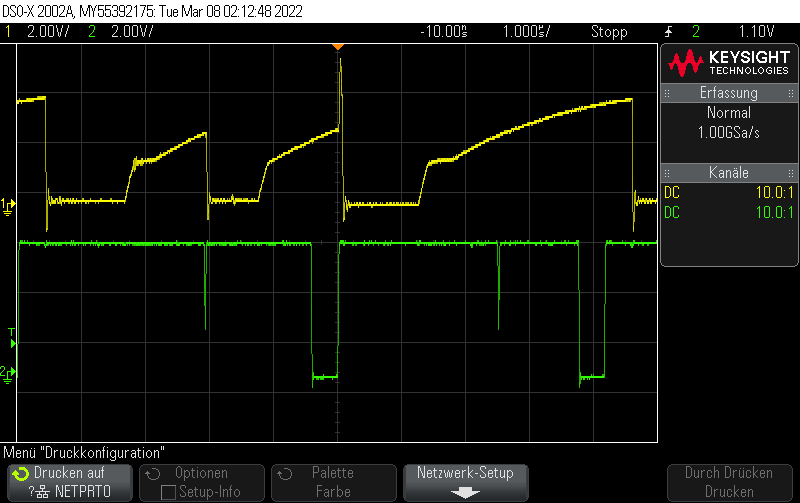
\includegraphics[width=\textwidth]{scope_9.png}
  \caption{Write Enable of \gls{MAR} register (green) and one bus lane without \texttt{0xff} driver (yellow).}
  \label{fig:busPullup}
\end{figure}
\begin{figure}[t]
  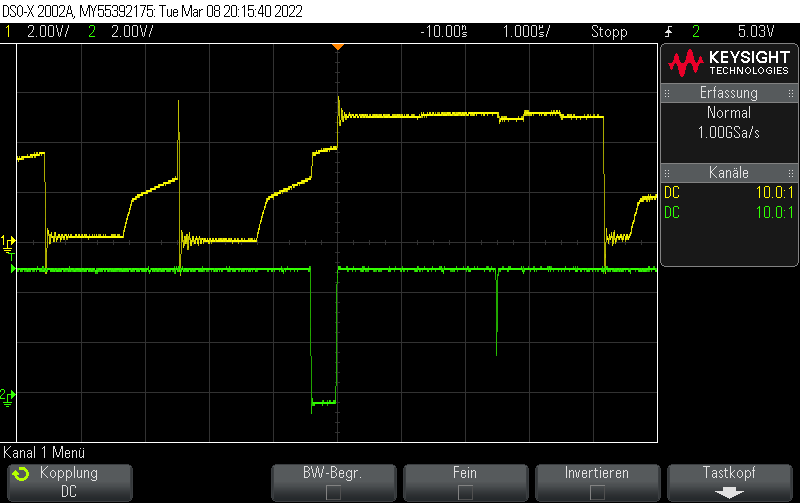
\includegraphics[width=\textwidth]{scope_10.png}
  \caption{Write Enable of \gls{MAR} register (green) and one bus lane with \texttt{0xff} driver (yellow).}
  \label{fig:busPullupFix}
\end{figure}
Until now, no program was programmed into the \glspl{EEPROM} and it was time for the first real integration test of the \gls{EDiC}.
The first program used for the integration test in \cref{lst:test0} was a basic test to see if basic instructions get executed and if the built-in I/O works.
After it ran successfully without any problems, the second testing program \cref{lst:test1} included the RS232 I/O extension card and its scratch register (at address \texttt{0xfe0f}).
When this also ran successfully, a more complex \gls{UART} echo program (\cref{lst:app_asm_uart}) was programmed into the \glspl{EEPROM}.
It finally had problems and did not work as expected.
However, when turning on the cycle by cycle debugger and stepping through all cycles, the program worked perfectly and bytes got read correctly from the RS232 extension card and were also sent correctly back.
After debugging for a long time the bug was tracked down to the return instruction which sometimes (about 1 in 100 times) would return to a random instruction and not return to after the call instruction.
It was further debugged with the third test program (\cref{lst:test2}).
With an oscilloscope it was finally possible to detect the problem which is shown in \cref{fig:busPullup}.
It is actually a bug in both, the call and return, which results in the same misbehavior of return to a wrong location:
Both instruction load \texttt{0xff} into the \gls{MAR} by not driving the bus with a specific value and relying on the pull-up resistors to pull the lines high.
In \cref{fig:busPullup} two \gls{MAR} write enable pulses can be seen and, especially, in the first pulse, the problem becomes apparent.
If the bus was pulled low in the cycle before the \gls{MAR} is written, the pull-up resistors take some time to pull the voltage to \qty{5}{\volt} which leaves the level at about \qty{2}{\volt} which is right at the required minimum voltage to be detected as a high signal by the \emph{74F825}.
Therefore, most of the time, the register detects the bus input as a 1 but sometimes it is detected as a low signal.

The fix is quite easy as soon as the problem is detected:
A new bus driver (\emph{74F245}) is added in one of the spare slots whose A input is connected to \texttt{H1}, the B input to the bus and the output enable signal is connected to a new control signal.
For this case it is always important to plan for many possibilities as this fix would have been very difficult if no output of the microcode \glspl{EEPROM} would be free to use or if no place for spare \glspl{IC} was left on the \gls{PCB}.
The result of the fix can be seen in \cref{fig:busPullupFix} where the bus line is raised to about \qty{3.8}{\volt} as soon as the write enable pulse starts\footnote{The even higher level on the bus line after the write enable pulse is driven by the \gls{SRAM} driver (outputs the return address in the return instruction) which is an \emph{ACT} type for compliance with the \gls{SRAM} specification. It is not seen in \cref{fig:busPullup} because it was a call instruction where the \gls{SRAM} does not drive the bus on the next cycle.}.

\subsection{\glsxtrshort{UART} Transceiver lost data}
The final bug was only observed with the test adapter and never while running the \gls{EDiC} on its own.
One of the integration tests was to manually write a value from the test adapter to the scratch register of the \gls{UART} \gls{IC} (TL16C550AN) on the RS232 extension card and then read it out repeatedly.
The observed result was that the data was read back successfully for a couple of times but often the data would be read back incorrectly after several reads.
However, the automated test with the program from \cref{lst:test1} the data was still correctly displayed at the built-in I/O after half an hour which results in about 300 million reads without errors\footnote{\qty{2.4}{\mega\hertz}, 14 cycles per loop iteration and 1800 seconds run time}:
\begin{equation}
  \frac{\qty{2.4}{\mega\hertz}}{14}\cdot\qty{1800}{\second}\approx 309\cdot 10^6
\end{equation}

\begin{figure}[t]
  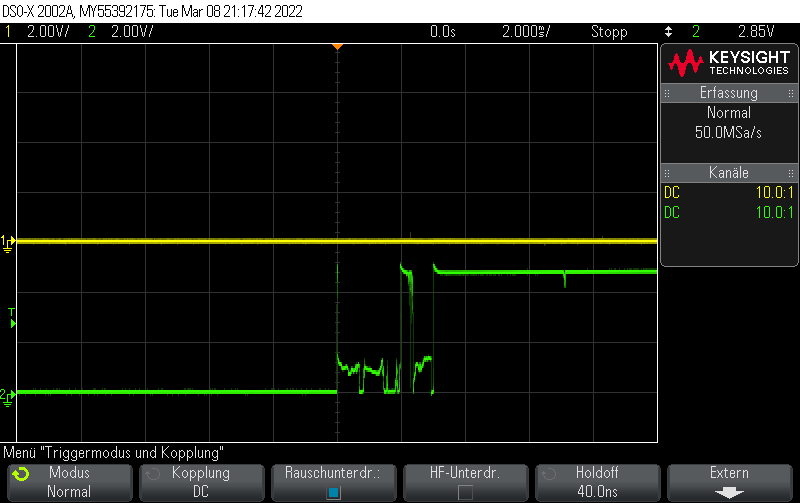
\includegraphics[width=\textwidth]{scope_12.png}
  \caption{DIP Switch output on switching (yellow).}
  \label{fig:bounce}
\end{figure}
The only notable difference between the two tests is that in the manual test, the output enable signal to the \gls{UART} \gls{IC} was set by hand with a DIP Switch and in the automated test, it was controlled by the output of the \gls{EEPROM}.
When looking at the waveforms of the signal coming from the DIP switch a bouncing of the trigger can sometimes be observed as shown in \cref{fig:bounce}.
In theory this should not have an effect on the content of the scratch register of the \gls{UART} \gls{IC} as the glitch happens on the output enable input of the \gls{IC}.
However, the datasheet explicitly states a minimum time for a read strobe pulse duration of \qty{80}{\nano\second}.
For this reason, the test adapter was altered to include a low pass filter and schmitt trigger on the \texttt{memRamNOE} and \texttt{memRamNWE} control signals because those are the only control signals which are used asynchronously.
All other control signal are only used in components which do not state a minimum pulse duration for it (only setup and hold times in relation to the rising edge of the clock).
After implementing this fix, the manual test worked perfectly for many read cycles which means that the minimum read pulse durations for the \gls{UART} \gls{IC} need to be respected.

\begin{figure}[t]
  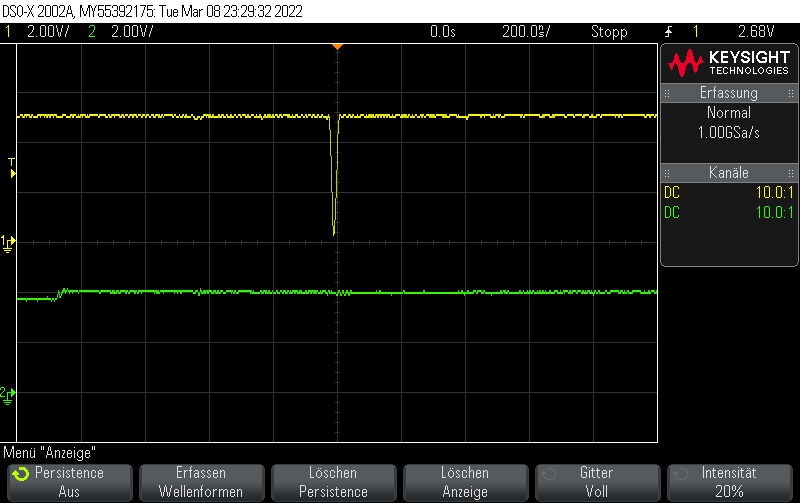
\includegraphics[width=\textwidth]{scope_15.png}
  \caption{Output of the \texttt{memRamNOE} control signal from the \gls{EEPROM} (yellow).}
  \label{fig:EEPROMGlitch}
\end{figure}
Even though, the problem never occurred with the control signals coming from the microcode \gls{EEPROM}, we looked into the specifications for the \gls{EEPROM} and found it also has a period after the address inputs change where the data output is undefined.
When observing the output with the oscilloscope, it was observed that there sometimes are glitches on the \texttt{memRamNOE} control signal as shown in \cref{fig:EEPROMGlitch}.
Therefore, it was decided to add a register to the \texttt{memRamNOE} and \texttt{memRamNWE} control signals.
This results in the microcode needing adjustment to assert these two signals one cycle earlier but was easy to implement and circumvent the problem completely.
% !TeX root = ../thesis.tex

\chapter{Conclusion and Future Work}\label{cha:conclusion}
This thesis presented the challenges of and solutions for designing and building a model \gls{CPU} for educational purposes.
It was shown that a simple and yet powerful \gls{CPU} can be developed using the easy-to-understand \gls{TTL} \glspl{IC} of the 74 family.
The most suitable architecture for this purpose has to be modularized and, therefore, a multicycle and single-bus oriented architecture was chosen.
By adding a more complex address logic for the memory, it was possible to extend the address space from 8 to 16 bits while maintaining a simpler 8 bit data bus.
The address logic also enabled versatile memory mapped \gls{IO} for arbitrary extension cards as shown with the RS-232 \gls{UART} extension card used in the demonstration in \cref{fig:EDiCSnake}.
Moreover, with a custom stack implementation the \gls{EDiC} is also able to implement function calls and function local variables.

One major contribution to ease the educational use of the \gls{EDiC} is the comprehensive software development environment which supports the custom \gls{EDiC} \gls{ISA}.
It consists of an assembler which is able to translate advanced human-readable assembler code to the 24 bit instructions used by the \gls{EDiC}.
Features such as value and string constants, file imports and label definitions support the programmer in creating software for the \gls{EDiC}.
Additionally, a tool to generate microcode for the \gls{EDiC} is provided.
Creating the memory contents for the microcode \glspl{EEPROM} of the \gls{EDiC} is a task that is very time-consuming and error-prone if done manually.
Therefore, a tool is provided which reads a human-readable file which describes all the instructions and what control signals are to be asserted in which cycle of the instruction.
A second tool converts the file to the memory contents for the \glspl{EEPROM}.

For quicker design iterations and also for verification of the finalized design, two \gls{FPGA} implementations were created in the process.
The first implementation is a behavioral implementation which was used to efficiently make alterations to the architecture in the design phase.
With the behavioral implementation, it was easy to design the \gls{CPU} on the logical level before diving into the details and mapping the logic onto discrete logic \glspl{IC}.
The second \gls{FPGA} implementation was used as a verification of the hardware schematic after it was created.
A specifically written software converted the netlist that was exported from the schematic tool to a \gls{HDL} description of the exact schematic.
All the logic \glspl{IC} were implemented as individual modules and an \gls{FPGA} design which is logically equivalent to the final hardware build could be simulated.
With the help of a small adapter from \gls{IO} of the \gls{FPGA} evaluation board to the extension board connector, it was possible to also test the extension card before ordering the large \gls{PCB} for the hardware build of the \gls{EDiC}.

When designing the final hardware build, the extensive simulation and testing of the \gls{FPGA} design simplified the required verification.
Additionally, a comprehensive timing analysis was performed to choose the correct clock frequency for the best performance while still ensuring that timing bugs do not occur at any time.
The hardware build includes custom designed test adapters which ease the initial hardware tests enormously.
With the test adapters and by using sockets for all logic \glspl{IC} it was possible to incrementally test the \gls{PCB} and discover some possible problems or bugs which slipped through the extensive logical simulation.

\section{Future Work}
Even though the \gls{EDiC} is a complex and yet simple to understand model \gls{CPU} with an extensive development environment, there are some more ideas that would enhance the \gls{EDiC} as a whole.

\paragraph{Power Supply} At the moment, the \gls{EDiC} is supplied by an industry standard 5V power supply.
However, with a custom-built \gls{CPU} made of discrete logic \glspl{IC} it would only be appropriate to also power the \gls{EDiC} with its own custom power supply.
Therefore, it is planned to design and build a power supply before the \gls{EDiC} will be presented at the \gls{VCFB}. \cite{vcfb}

\paragraph{Extension Cards} The \gls{EDiC} currently only has the RS-232 \gls{UART} extension card.
This is one of the most versatile extensions as it can be connected to a lot of different devices and thus providing a communication interface to the outside world via a standardized serial protocol.
However, a lot more possible extensions could be used such as an extension card to provide a persistent storage or the capabilities of the \gls{ALU} could be enhanced by providing a multiply extension or other computational hardware in the form of extension cards.

\paragraph{High Level Language Compiler} The most complex software which currently exists for the \gls{EDiC} is the snake program.
However, writing more complex software in assembler is of course possible but becomes increasingly hard and takes a lot of programming effort.
Therefore, a possible addition is to implement a compiler which could translate a high level programming language like C to \gls{EDiC} assembler or machine code.
With modular compiler infrastructure as it is provided by the LLVM it may be possible to create a compiler backend for the \gls{EDiC}.


\cleardoublepage
\printglossary[type=\acronymtype]

% das Abbildungsverzeichnis
\listoffigures
\addcontentsline{toc}{chapter}{List of Figures}

% das Tabellenverzeichnis
\listoftables
\addcontentsline{toc}{chapter}{List of Tables}

% list of listing
\listoflistings
\addcontentsline{toc}{chapter}{\listoflistingscaption}

% Literaturverzeichnis
\printbibliography
% \raggedright
% \bibliography{bib.bib}{}
% \bibliographystyle{numeric}

\appendix
\chapter{Collection of assembler programs for the \gls{EDiC}}
\begin{multipagecode}
  \caption{The full snake assembler program.}
  \begin{multicols}{2}
    \inputminted[linenos,
      breaklines,
      frame=leftline,
      xleftmargin=20pt,
    ]{ARM}{src/snake.s}
  \end{multicols}
  \label{lst:app_asm_snake}
\end{multipagecode}

\begin{multipagecode}
  \caption{The \gls{PRNG} assembler program ``prng.s'' used in the snake program in \cref{lst:app_asm_snake}.}
  \inputminted[linenos,
    breaklines,
    frame=leftline,
    xleftmargin=20pt,
  ]{ARM}{src/prng.s}
  \label{lst:app_asm_prng}
\end{multipagecode}

\begin{multipagecode}
  \caption{The utility library for the \gls{UART} extension card of the \gls{EDiC} with the \texttt{16c550} \gls{UART} Transceiver.}
  \begin{multicols}{2}
    \inputminted[linenos,
      breaklines,
      frame=leftline,
      xleftmargin=20pt,
    ]{ARM}{src/uart_16c550.s}
  \end{multicols}
  \label{lst:app_asm_uart}
\end{multipagecode}

\chapter[Collection of assembler programs]{Collection of assembler programs for the \gls{EDiC}}
\begin{multipagecode}
  \caption{The full snake assembler program.}
  \begin{multicols}{2}
    \inputminted[linenos,
      breaklines,
      frame=leftline,
      xleftmargin=20pt,
    ]{ARM}{src/snake.s}
  \end{multicols}
  \label{lst:app_asm_snake}
\end{multipagecode}

\begin{multipagecode}
  \caption{The \gls{PRNG} assembler program ``prng.s'' used in the snake program in \cref{lst:app_asm_snake}.}
  \inputminted[linenos,
    breaklines,
    frame=leftline,
    xleftmargin=20pt,
  ]{ARM}{src/prng.s}
  \label{lst:app_asm_prng}
\end{multipagecode}

\begin{multipagecode}
  \caption{The utility library for the \gls{UART} extension card of the \gls{EDiC} with the \texttt{16c550} \gls{UART} Transceiver.}
  \begin{multicols}{2}
    \inputminted[linenos,
      breaklines,
      frame=leftline,
      xleftmargin=20pt,
    ]{ARM}{src/uart_16c550.s}
  \end{multicols}
  \label{lst:app_asm_uart}
\end{multipagecode}

\end{document}
%%%%%%%%%%%%%%% END %%%%%%%%%%%%%%%
